\documentclass{jfm}

\usepackage{graphicx}
\usepackage{natbib}
\usepackage{hyperref}
\usepackage{amsmath}
\usepackage{ar}
\usepackage{tikz}
\usepackage{pgfplots}
\usepackage{tikz-3dplot}
\usepackage{bm}
\usepackage{multirow}
\usepackage{subfig}
\usepackage{overpic}
\usepackage[normalem]{ulem}

\newcommand{\aver}[1]{ \! \left\langle {#1} \right \rangle \!}




\begin{document}
\title{On the secondary bifurcation of the flow past rectangular cylinders}
\author{Alessandro Chiarini and Emanuele Gallorini}
\affiliation{Dipartimento di Scienze e Tecnologie Aerospaziali, Politecnico di Milano, via La Masa 34, 20156 Milano, Italy}
\maketitle

\section{Introduction}

The flow past bluff bodies and the formation of vortex structures in their wake has attracted the attention of many scholar over the last decades, as they are ubiquitous in natural environments and in several engineering applications \citep{oertel-1990,williamson-1996b,choi-etal-2008,thompson-etal-2021}. Two-dimensional and symmetric bluff bodies isolated in free stream are the prototype of this kind of flows.

Most studies on 2D bluff bodies have focused on the circular and square cylinders to characterise the flow bifurcations. The low-$Re$ steady flow generally becomes unstable to oscillatory perturbations that lead to the von K\'{a}rm\'{a}n vortex shedding. The wake past a circular cylinder, for example, undergoes a Hopf bifurcation at a Reynolds number of $Re = U_\infty D /\nu = 47$, where $U_\infty$ is the free stream velocity and $D$ is the radius of the cylinder \cite{noack.eckelmann-1994-globalstability}. This first Hopf bifurcation is generic to flows past isolated 2D bodies that respect the top/down reflectional symmetry \citep{jackson-1987-finiteelementstudy,chiarini-quadrio-auteri-2022b}. The triggering mechanism of this bifurcation is known to result from a global instability \citep{jackson-1987-finiteelementstudy}, which arises when the region of local absolute instability is large enough \citep{chomaz-2005}. Accordingly, \cite{chiarini-quadrio-auteri-2022b} observed that the onset of this instability depends on the size of the wake recirculating region and on the maximum reverse flow velocity.
%
The secondary instability of the wake past 2D symmetric bluff bodies is generally thought to lead to a three-dimensional flow. For the circular cylinder, for example, the periodic von K\'{a}rm\'{a}n wake undergoes a secondary pitchfork bifurcation at $Re \approx 190$: the flow becomes three-dimensional but retains the same periodicity. \cite{barkley-henderson-1996} found by Floquet stability analysis that the two-dimensional von K\'{a}rm\'{a}n wake becomes unstable to the synchronous three-dimensional mode $A$ which has spanwise wavelength $\lambda \approx 3.9 D$ at $Re \approx 190$, and to mode $B$ with $\lambda \approx 1.2 D$ at slightly larger $Re$. The following studies of \cite{henderson-barkley-1996} and \cite{henderson-1997} showed that the onset of modes $A$ and $B$ are due to a supercritical and subcritical bifurcation, respectively. A quasi-periodic mode $S$ with $\lambda \approx 2.5D$ has been also found to become unstable at larger $Re$ \citep{blackburn-lopez-2003,blackburn-etal-2005,blackburn-sheard-2010}. 
%
\cite{ryan-thompson-hourigan-2005} investigated the secondary instability of the flow past streamlined elongated cylinders (the flow does not separate at the LE in these cases), and found that the secondary bifurcation leads to a 3D flow for all cases. However, they found that the most unstable mode, and therefore the sequence of bifurcations the flow unergoes, changes with the aspect ratio $\AR=L/D$ of the body. They found mode $A$ and two new modes, called mode $B'$ and $S'$ in analogy with the circular cylinder case. Mode $B'$ possesses the same spatio-temporal symmetry as mode $B$, but a spanwise wavelength and near-wake features that are more similar to mode $S$. Mode $S'$ is time-varying from one shedding period to the next one, similarly to mode $S$ for the square and circular cylinder \citep{robichaux-balachandar-vanka-1999}, but exhibits a perturbation field that is reminiscent of mode $B$. \cite{ryan-thompson-hourigan-2005} observed that for small aspect ratios, i.e. $\AR \le 7.5$, the first mode to become unstable is mode $A$, while for larger $\AR$ the first mode to become unstable is $B'$. 

We now move to two-dimensional symmetric bluff bodies with sharp LE corners, that are the focus of the present work. Unlike circular and streamlines cylinders, in this case the presence of the corners at the LE enforces the flow separation. The flow past rectangular cylinders with blunt LE is the prototype of this kind of flows, and has been largely investigated over the last years at both (relatively) low \citep{hourigan-thompson-tan-2001,zhang-etal-2023} and and large \citep{cimarelli-leonforte-angeli-2018,chiarini-etal-2022,cimarelli-etal-2024} Reynolds numbers. Varying the aspect ratio a wide range of bodies is obtained, from a flat placed placed normal to the incoming flow for $\AR \rightarrow 0$, to a flat plate parallel to the incoming flow for $\AR \rightarrow \infty$. Notably, already at intermediate Reynolds numbers after the primary Hopf bifurcaton, i.e. $Re \approx 200-400$, the flow physics is extremely rich and largely depends on $\AR$ \citep[see for example][]{okajima-1982,nakamura-etal-1991,mills-etal-1995}. For $\AR \le 1$ the shear layers that separate at the LE roll up in the wake and create the classical von K\'{a}rm\'{a}n vortex street; in this case the flow dynamics resembles that of the circular cylinder case. For intermediate aspect ratios, i.e. $1 \le \AR \le 3$, the shear layers separating from the LE reattach intermittently over the lateral sides of the cylinder: a recirculating region intermittently arises there. For larger $\AR$, instead, the LE shear layers reattach along the top/bottom lateral sides of the cylinder permanently, and generate large recirculating regions that periodically enlarge and shrink. At large enough $Re$, for these larger $\AR$ vortex shedding occurs from both the LE and TE shear layers and the two phenomena lock to the same frequency due to the so-called ILEV instability, leading to an almost stepwise dependence of the Strouhal number $St_L=fL/U_\infty$ on $\AR$ \citep{okajima-1982,nakamura-etal-1991,hourigan-thompson-tan-2001}; see figure \ref{fig:StLAR}. 
%
\begin{figure}
  \centering
   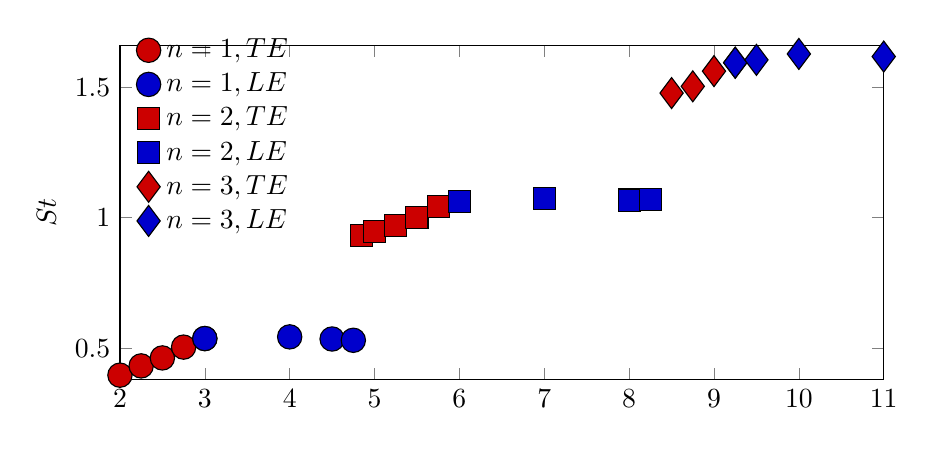
\begin{tikzpicture}



\begin{axis}[%
%width=4.3cm,
%height=3.5cm,
width=0.8\textwidth,
height=0.35\textwidth,
scale only axis,
%grid=both,
%axis lines=middle,
xmin=2,
xmax=11,
ymin=0.38,
ymax=1.66,
%xtick={2, 3, 4, 5, 6, 7, 8, 9, 10, 11},
%ytick={0.4, 0.6, 0.8, 1, 1.2, 1.4, 1.6, 1.8},
%xlabel style={font=\color{white!15!black}},
xlabel={\AR},
ylabel={$St$},
%ymin=0,
%ymax=200,
axis background/.style={fill=white},
legend style={at={(0.01,0.73)}, anchor=west, legend cell align=left, align=left, fill=none, draw=none}
]

\addplot [color=black,only marks,mark=*,mark options={scale=2.2,black,fill=red!80!black}]
  table[row sep=crcr]{%
2       0.396741726829078\\
2.25    0.432248406188668\\
2.5     0.462793383468913\\
2.75    0.504214143890634\\
3       0.536994008053543\\
};
\addlegendentry{$n=1,TE$}

\addplot [color=black,only marks,mark=*,mark options={scale=2.2,black,fill=blue!80!black}]
  table[row sep=crcr]{%
3       0.536994008053543\\
4       0.543439544221324\\
4.5     0.535298051494477\\
4.75    0.530324957725253\\
};
\addlegendentry{$n=1,LE$}


\addplot [color=black,only marks,mark=square*,mark options={scale=2,black,fill=red!80!black}]
  table[row sep=crcr]{%
4.85    0.930407996044941\\
5       0.947349623285183\\
5.25    0.971304878725648\\
5.5     1.000378564453700\\
5.75    1.041747167637721\\
6       1.062464533558995\\
};
\addlegendentry{$n=2,TE$}

\addplot [color=black,only marks,mark=square*,mark options={scale=2,black,fill=blue!80!black}]
  table[row sep=crcr]{%
6       1.062464533558995\\
7       1.073230579537877\\
8       1.067458930414985\\
8.25    1.070000000000000\\
};
\addlegendentry{$n=2,LE$}


\addplot [color=black,only marks,mark=diamond*,mark options={scale=2.8,black,fill=red!80!black}]
  table[row sep=crcr]{%
8.5     1.477258532919061\\
8.75    1.503123920971757\\
9       1.561211928154617\\
9.25    1.593577708455838\\    
};
\addlegendentry{$n=3,TE$}

\addplot [color=black,only marks,mark=diamond*,mark options={scale=2.8,black,fill=blue!80!black}]
  table[row sep=crcr]{%
9.25    1.593577708455838\\    
9.5     1.604355188881951\\
10      1.627228310690177\\
11      1.617135083478177\\
};
\addlegendentry{$n=3,LE$}



%\addplot [color=black,solid,mark=square*,mark options={scale=0.9,black,fill=red!80!black}]
%  table[row sep=crcr]{%
%3       0.609743754434522\\
%4       0.774727821194389\\
%5       0.942866305443131\\
%6       1.100079139112736\\
%7       1.245663824885169\\
%8       1.400191666484032\\
%9       1.546133959599630\\
%10      1.685632118301302\\
%11      1.822225132985195\\
%};



\end{axis}


\end{tikzpicture}%

   \caption{Dependence of $St_L$ on $\AR$ at $Re=400$. Figure adapted from \cite{chiarini-quadrio-auteri-2022}.}
   \label{fig:StLAR}
\end{figure}
%
This stepwise change of $St_L$ is related to the number $n$ of LE vortices that are simultaneously accommodated along the lateral sides of the cylinder, being for example $n=1$ for $\AR=4$, $n=2$ for $\AR=7$ and $n=3$ for $\AR=9$. \cite{chiarini-quadrio-auteri-2022} observed that two different regimes are possible depending on the relative phase between the LE and TE vortices and on the prevalence of either shedding. When the LE vortices dominate the shedding frequency locks to the passing frequency of the LE over the TE and $St \approx n U_c$, where $n$ is the number of LE vortices present simultaneously over the sides of the cylinder and $U_c \approx 0.55 U_\infty$ is the mean convection velocity of the LE vortices \citep[see also][]{mills-sheridan-hourigan-2002,tan-thompson-hourigan-2004}. In contrast, when the TE vortices dominate the flow matches the frequency of elongated bodies with same $\AR$, but rounded LE that does not produce flow separation. Using dynamic mode decomposition, \cite{zhang-etal-2023} observed that the feedback mechanism at $Re = 1000$ changes with $\AR$. For small $\AR$, the feedback loop encompasses the whole separation region and the flow is controlled by the impinging shear-layer instability; for larger $\AR$, the feedback loop covers the entire chord of the cylinder and the flow is controlled by the leading-edge vortex shedding instability.
  
The presence of different regimes and LE/TE vortex interactions hints for the existence of different secondary instabilities and thus different routes to turbulence. To the best of our knowledge, however, a complete picture is still missing and little is known about the secondary instability of the flow past elongated rectangular cylinders with $\AR>1$. It is well established that the flow past a square cylinder ($\AR=1$) undergoes the same sequence of bifurcations mentioned for the circular cylinder case, albeit the primary and secondary instabilities occur at a slightly lower Reynolds number \citep[see for example][]{jiang-cheng-2018,blackburn-sheard-2010}. Indeed, \cite{robichaux-balachandar-vanka-1999}, \cite{blackburn-lopez-2003}, \cite{sheard-fitzgerald-ryan-2009}, \cite{blackburn-sheard-2010} found via Floquet stability analysis that the flow becomes $3D$ due to mode $A$ at $Re \approx 165$, and that modes $B$ and $S$ become unstable only at larger $Re$. By means of 3D Direct Numerical Simulations (DNS), \cite{sheard-fitzgerald-ryan-2009} and \cite{jiang-cheng-an-2018} discussed the saturation effect of the nonlinear terms on the growth of the different modes. \cite{sheard-fitzgerald-ryan-2009} found that the appearance of both modes $A$ and $B$ is due to a supercritical bifurcation. However, \cite{jiang-cheng-an-2018} remarked that, unlike the circular cylinder case \citep{henderson-1997}, the instability of mode A is subcritical; they explained the discrepancy with the results of \cite{sheard-fitzgerald-ryan-2009} with the small computational domain adopted in the latter study. \cite{sheard-fitzgerald-ryan-2009} and \cite{sheard-2011} studied how the angle of incidence affects the unstable modes: mode $A$ is the most unstable one at small and large incidences, while a subharmonic mode, called $C$, is the most unstable at intermediate angles. \cite{choi-yang-2014} considered the flow past rectangular cylinder with $\AR \le 1$, ranging from a flat plate normal to the flow ($\AR \rightarrow 0$) to a square cylinder ($\AR=1$). They found that when reducing $\AR$ both modes $A$ and $B$ stabilise and that new modes A2 and QP2 of synchronous and quasi periodic nature become unstable \citep[see also][]{thompson-etal-2006}. \cite{chaurasia-thompson-2011} and \cite{huang-etal-2017} studied the flow past a semi-indefinite plate of finite thickness, i.e. a rectangular cylinder with $\AR \rightarrow \infty$. The found that the vortices that arise from the LE shear layer due to an induced Kelvin--Helmholtz instability become unstable to subharmonic 3D perturbations at $Re \approx 380$. Despite these works, however, almost no information is available for the secondary bifurcation of the flow past elongated rectangular cylinders with $1 < \AR < \infty$. In a recent work \citep{chiarini-quadrio-auteri-2022d}, we have considered the specific $\AR=5$ ($n=2$ regime dominated by the TE vortex shedding) that defines the BARC benchmark, and found that the secondary instability is due to the QS mode which is of quasi subharmonic nature. Specifically, we found that the wavemaker \citep{monkewitz-huerre-chomaz-1993} of this instability is localised in the region over the longitudinal sides of the cylinder, and that the instability is triggered by the mutual inviscid interaction of the vortices generated by the LE shear layer. It is thus clear that a complete characterisation of how the different flow regimes and LE/TE vortex interaction influence the secondary instability of the flow past rectangular cylinder with $\AR>1$ and thus its route to turbulence is lacking.
    
The aim of this work is to do a step forward in this direction. We aim to fill the gap and characterise the secondary bifurcation of the flow past rectangular cylinders with $1 \le \AR \le 9$ by means of both stability analysis and fully nonlinear 3D DNS. In this work, besides characterising how the different LE/TE vortex interactions influence the bifurcation scenario, we will also provide insights on the triggering mechanism of mode $A$. As shown in the following, indeed, mode $A$ is found only in the regimes dominated by the TE vortices. 
  
The remainder of the work is structured as follows ...
  
\section{Mathematical formulation and numerical methods}
\label{sec:methods}

\subsection{Flow configuration}
The incompressible flow past rectangular cylinders with aspect ratio $\AR=L/D$, where $L$ and $D$ indicate their length and thickness, is considered. A Cartesian coordinate system centred at the LE of the cylinders is used. The $x$ direction is aligned with the free-stream flow direction, and $y$ denotes the cross-stream direction. When present, $z$ is the spanwise direction. The cylinders are placed in a uniform flow with velocity $\bm{U}=U_\infty\hat{\bm{e}}_x$. The Reynolds number depends on the incoming flow and on the cylinder thickness, and is defined as $Re= U_\infty D /\nu$, where $\nu$ is the kinematic viscosity. The flow is governed by the incompressible Navier--Stokes equations, i.e.
%

\begin{equation}
\begin{cases}
\frac{\partial U}{\partial t} + \bm{U} \cdot \bm{\nabla}\bm{U} = - \bm{\nabla} P + \frac{1}{Re} \nabla^2 \bm{U} \\
\bm{\nabla} \cdot \bm{U} = 0
\end{cases}
\label{eq:NSequations}
\end{equation}
%
where $\bm{U}$ is the velocity vector with components $\bm{U}=(U,V,W)$ and $P$ is the reduced pressure. No-slip and no-penetration boundary conditions are imposed at the cylinder side, while undisturbed velocity is enforced at the inlet and at the farfield. At the outlet convective boundary conditions
% 
\begin{equation*}
P \bm{n} - \frac{1}{Re} \bm{\nabla} \bm{U} \cdot \bm{n} = \bm{0}
\end{equation*}
%
are used. Periodic boundary conditions are used in the spanwise direction to account for homogeneity.

\subsection{Floquet analysis}

Floquet theory is used to study the linear stability of 2D time-periodic base flows to three-dimensional perturbations. The flow field $\{\bm{U},P\}$ is written as the sum of the a 2D periodic base flow $\{\bm{U}_b,P_b\}$ and an unsteady 3D perturbation of small amplitude $\epsilon$:
\begin{equation}
\{\bm{U},P\}(x,y,z,t) = \{\bm{U}_b,P_b\}(x,y,t) + \epsilon \int_{-\infty}^{\infty} \{\bm{u},p\}(x,y,\beta,t) \text{e}^{i \beta z} \text{d} \beta;
\end{equation}
here $i$ is the imaginary unit, $\bm{u}$ and $p$ indicate the Fourier transform of the velocity and pressure perturbations in the homogeneous $z$ direction and $\beta$ is the corresponding wavenumber.

Introducing this decomposition in \ref{eq:NSequations} the governing equations for the base flow are obtained at order $\epsilon^0$, that are the two-dimensional incompressible Navier--Stokes equations, while the eigenproblem describing the evolution equation for the perturbations are obtained at order $\epsilon^1$. They are the linearised Navier--Stokes equations (LNSEs) that for each $\beta$ read:
%
\begin{equation}
\begin{cases}
\frac{\partial \bm{u}}{\partial t} + \mathcal{L}_\beta\{\bm{U}_b,Re\}\bm{u} + \bm{\nabla}_\beta p = 0 \\
\bm{\nabla}_\beta \cdot \bm{u} = 0
\end{cases}
\label{eq:LNSEs}
\end{equation}
%
where $\bm{\nabla}_\beta \equiv (\partial / \partial x,\partial / \partial y, i\beta)$ is the Fourier-transformed gradient operator and $\mathcal{L}_\beta$ is the Fourier-transformed linearised Navier--Stokes operator:
%
\begin{equation}
\mathcal{L}_\beta\{\bm{U}_b,Re\}\bm{u}=\bm{U}_b \cdot \bm{\nabla}_\beta \bm{u} + \bm{u} \cdot \bm{\nabla}_\beta \bm{U}_b - \frac{1}{Re} \nabla^2_\beta \bm{u},
\end{equation}
%
where $\nabla^2_\beta \equiv \nabla_\beta \cdot \nabla_\beta$ is the Fourier-transformed Laplacian operator. Following the Floquet theory we further decompose the perturbation field into:
%
\begin{equation}
\{\bm{u},p\}(x,y,\beta,t) = \{\hat{\bm{u}},\hat{p}\}(x,y,\beta,t) \text{e}^{\sigma t}
\end{equation}
%
where $\sigma$ is the Floquet exponent and $\{ \hat{\bm{u}},\hat{p} \}$ is the associated Floquet mode, that has the same periodicity as the base flow. The stability of the system is determined by the sign of the real part $\Re(\sigma)$ of the Floquet exponent, or equivalently, by the modulus of the Floquet multiplier $\mu = e^{\sigma T}$. If all $\Re(\sigma)<0$, or $|\mu<1|$, the system is stable and the perturbations decay. If one exponent exist with $\Re(\sigma)>0$, or $|\mu>1|$ the perturbation grows exponentially; if $\beta \neq 0$ the flow becomes three-dimensional.

\subsection{Computational details}

In the present work we use two distinct numerical methods. The stability analysis is carried out using a numerical code based on finite elements and implemented in the non-commercial software FreeFem++ \citep{hecht-2012}; see \cite{chiarini-quadrio-auteri-2022d} and \cite{chiarini-nastro-2025} for details. The 3D fully non linear simulations are instead carried out with an in-house solver based on finite differences, which has been already used to study the flow past 2D and 3D bluff bodies in both the laminar and turbulent regimes \citep{chiarini-quadrio-auteri-2022d,chiarini-boujo-2024,chiarini-etal-2022}.

The 2D time-periodic base flows $\{\bm{U}_b,P_b\}$ are evaluated by integrating in time the two-dimensional discretised version of the Navier--Stokes equations \ref{eq:NSequations}. The time integration employs an explicit thir-order, low-storage Runge--Kutta method for the non-linear term, combined with an implicity second-order Crank--Nicolson scheme for the linear terms \cite{rai-moin-1991}. The non-commercial, finite-element software FreeFem++ is employed to discretise the equations. Triangular quadratic elements and linear elements are used for the velocity vector and the pressure to satisfy the LBB condition \citep{brezzi-1974}. The BoostConv algorithm \citep{citro-etal-2017} accelerates the convergence of the simulations to the periodic limit cycle; for all cases the base flow is verified to satisfy the requires spatio-temporal symmetries 
\begin{equation}
\{U_b,V_b,P_b\}(x,y,z,t) = \{U_b,-V_b,P_b\}(x,-y,z,t+T/2)
\end{equation}
up to a threshold of $10^{-10}$. The computational domain extends for $-25 D\le x \le 60 D$ in the stremwise direction and for $-40 D \le y \le 40 D $ in the cross-stream direction, leading to $L_x=85D$ and $L_y=80D$. A symmetric grid with respect to the $x$ axis is used to avoid introducing spurious asymmetries in the flow. The number of triangles slightly changes with $\AR$, from a minimum of $8 \times 10^4$ to a maximum of $18 \times 10^4$, and are distributed in order to properly refine the area close to the cylinders and the wake region.

The numerical method used for the Floquet analysis resembles that used by other authors \citep[see for example][]{barkley-henderson-1996}. The Floquet multipliers $\mu_\beta$ and the Floquet modes $\hat{\bm{u}}_\beta(t_0)$ at time $t_0$ of the operator $\mathcal{L}_\beta$ are the eigenvalues and eigenvectors of the linearised Poincarè map $\mathcal{P}_\beta$ that links the velocity perturbation $\bm{u}_\beta(t_0)$ with its evolution after one period, i.e.
%
\begin{equation}
\bm{u}_\beta(t_0+T) = \mathcal{P}_\beta \bm{u}_k(t_0).
\end{equation}
%
The eigenvalues of $\mathcal{P}_\beta$ with larger modulus and the associated eigenvectors have been computed with the Arnoldi method \citep{saad-2011}. The action of $\mathcal{P}_\beta$ on the initial perturbation $\bm{u}_\beta(t_0)$ is obtained integrating in time the LNSEs (equation \ref{eq:LNSEs}) from $t_0$ to $t_0+T$, using the same numerical scheme used for the computation of the base flow. The Gram-Schimdt algorithm is used for the eigenvectors orthogonalisation and all the computed modes are normalised using their total kinetic energy. During the integration of the LNSEs, the base flow is evaluated at each time step by the Fourier interpolation of 100 instantaneous fields stores equispaced in time over one period T.

The 3D Direct Numerical Simulations have been carried out using a numerical code introduced by \cite{luchini-2013}. It integrates in time the three-dimensional Navier--Stokes equations written in primitive variables on a staggered grid using finite-differences in the three directions. The governing equations are advanced in time using a fractional time-stepping method with a third-order Runge-Kutta scheme. The Poisson equation for the pressure is solved using an iterative SOR algorithm. The presence of the cylinder is dealt with a second-order implicit immersed-boundary method \citep{luchini-etal-2025}. For these simulations the computational domain has size $L_x=XXD$, $L_y=XXD$ and $L_z=2\pi D$. The number of points slightly changes with $\AR$, being $(N_x,N_y,N_z) = (XX,XX,XX)$ for $\AR \in (1,3)$, $(N_x,N_y,N_z)=(XX,XX,XX)$ for $\AR =4.5$ and$(N_x,N_y,N_z)=(1040,570,200)$ for $\AR=5.5 $ and $\AR=7$ for a total of about 120 millions points. Their distribution is homogeneous in the spanwise direction, whereas a geometric progression is used the streamwise and vertical directions to properly refine the grid near the cylinders' corners and in the wake region. For all cases the cell size in correspondence of the corners is $\Delta x = \Delta y \approx 0.005D$. All the simulations are advanced in time using a variable timestep to enforce that the Courant–Friedrichs–Lewy number is below unity. 

Hereinafter, if not otherwise indicated, all variables are in dimensionless form with $D$ as length scale, $U_\infty$ as velocity scale and $D/U_\infty$ as time scale.

\section{What we can do}

\subsection{Strouhal-Reynolds-AR}

It would be interesting to parametrise the $St-Re$ dependence using $\AR$ as a parameter. This would provide a clear visualisation of the successive bifurcations the flow experiences.

\subsection{Neutral curves}

For the 3D bifurcations it would be more effective to draw the neutral curves in the $\beta-Re$ parameter space.


\subsection{Supercritical versus Subcritical bifurcations}

We can assess which is the nature of the bifurcations the flow experiences. For example, we can follow the approach described by Henderson \& Barkley (1996) for the pitchfork bifurcations; see also Henderson (1997).

To assess whether the bifurcation is subcritical or supercritical, we have to look at the influence of the nonlinearity for $Re \rightarrow Re_c$. We now focus on the pitchfork bifurcations. The normal form for a pitchfork bifurcation of a discrete-time dynamical system is
%
\begin{equation}
  A_{n+1} = \mu A_n + \alpha_1 A_n^3 + O(A_n^5)
\end{equation}
%
where $A_n$ corresponds to the real amplitude of the bifurcating flow at period $n$ and $\alpha_1$ is the Landau constant. When $\alpha_1<0$ the instability is a supercritical bifurcation. When $\alpha_1>0$, the instability is a subcritical bifurcation. In this case the transition is discontinuous and hysteretic.

We have to perform direct numerical simulations at $Re \approx Re_c$ using the full $2D$ nonlinear Navier--Stokes equations. Indeed, the most precise and direct way to analyse the nonlinear growth of the critical mode is to follow the evolution of initial conditions of the form $\bm{U}_b + \bm{u}_c$, where $\bm{u}_c$ is the Floquet mode at criticality. Moreover, since the initial conditions is characterised by a single wavenumber $\beta_c$, it is clear that due to the properties of the Navier--Stokes equations it is sufficient to retain in the NS equations only those modes with $\beta = m \beta_c$, where $m$ is an integer. This allows to not perform an actual 3D simulation.
The amplitude $A_n$ at this point may be simply considered as
%
\begin{equation}
  A_n \equiv =  \left( \frac{1}{\Omega U_\infty^2} \int_{\Omega} |\bm{u}^n_c|^2 \text{d} \Omega \right)^{1/2}
\end{equation}
%
where $\Omega$ is the area of the computational domain, and $\bm{u}^n_c$ is the Fourier coefficient of the velocity field at period $n$ and wavenumber $\beta_c$. In doing this, we can then plot $A_n$ as a function of the iteration and then evaluate the value of $\alpha_1$ as
%
\begin{equation}
  \alpha_1 \approx \frac{ A_{n+1} - \mu A_n}{A_n^3}.
\end{equation}
%

Clearly, in the case where the bifurcation is two-dimensional the approach is rather easy. In this case, indeed, $\beta_c = 0$. For three-dimensional bifurcations, instead, the situation is more complex and we should choose in somehow the number of mode to include in the 3D non linear simulations such that $m\le M$.

In the case the bifurcations are subcritical we should study the bi-stability interval.


For the specific case of the circular cylinder mode A is subcritcal, while mode B is supercritical.


Another possible approach to study the non linear effect is to carry out DNS close to the onset of the bifurcation.

\subsubsection{3D pitchfork}

After the flow bifurcation we can write
%
\begin{equation}
  \bm{U}(\bm{x},t) = U(t) \bm{\phi}_0(\bm{x},t) + A(t) \bm{\phi}_1(\bm{x},t).
\end{equation}
%
The idea is to study how non linearity influences the values of $U$ and $A$ in time. This would allow us to understand whether the bifurcations is subcritical or supercritical.

The idea is to decompose the velocity and pressure field using a Fourier decomposition, i.e.
%
\begin{equation}
  \bm{U}(\bm{x},t) = \sum_{j=0}^M \hat{\bm{u}}_j e^{i j \beta_c z} = \hat{\bm{u}}_0(\bm{x},t) + \hat{\bm{u}}_1(\bm{x},t) e^{i \beta_c z}+
                     \sum_{j=2}^M \hat{\bm{u}}_j e^{i j \beta_c z} 
\end{equation}
%
where $\beta_c$ is the critical wavenumber (result of the Floquet analysis). $\hat{\bm{u}}_0(\bm{x},t)$ denotes the spatial average and describes the evolution of the two-dimensional base flow. $\hat{\bm{u}}_1(\bm{x},t)$ denotes the coefficient associated with the Fourier mode having $\beta = \beta_c$.

At this point, we use as initial condition 
%
\begin{equation}
  \hat{\bm{u}}_0(\bm{x},t_n) = \bm{U}_b(\bm{x},0)
\end{equation}
%
where $\bm{U}_b$ denotes the saturated base flow evaluated with the non linear 2D Navier--Stokes equations, and
%
\begin{equation}
  \hat{\bm{u}}_1(\bm{x},t_n) = \bm{u}_{Fl}(\bm{x},0)
\end{equation}
%
where $\bm{u}_{Fl}$ denotes the most unstable Floquet mode.
We then integrate this initial condition using the complete, 3D and non linear Navier--Stokes equations to detect the effect of the non linearity on the bifurcation. In particular, we track the values of $U_n$ and $A_n$ as
%
\begin{equation}
  |U_n|^2 = \frac{1}{\Omega U_\infty^2} \int_{\Omega} | \hat{\bm{u}}_0(\bm{x},t_n |^1 \text{d}\Omega
\end{equation}
%
and
\begin{equation}
  |A_n|^2 = \frac{1}{\Omega U_\infty^2} \int_{\Omega} | \hat{\bm{u}}_1(\bm{x},t_n |^1 \text{d}\Omega
\end{equation}
%
where $A_n=A(t_n)$ and $t_n$ is such that $C_\ell(t_n) = 0$. Note that in doing this it is possible that the period of the oscillation actually changes due to the influence of the nonlinearity.

This allows as to evaluate whether the bifurcation is supercritical or subcritical. In fact, the normal form for a picthfork bifurcation is
%
\begin{equation}
  A_{n+1} = \left( \mu_1 + \sum_j \alpha_{ij}A_n^{2j} \right) A_n
\end{equation}
%
and the value of $\alpha_{11}$ determines whether the bifurcation is supercritical ($\alpha_{11}<0$) or subcritical ($\alpha_{11}>0$). Note that $\mu_1 = 1 + \mu'\epsilon$ where $\mu' = \text{d}\mu/\text{d}\epsilon$ and $\epsilon = (Re - Re_c)/Re_c$ is the small parameter.

At this point, by comparing the found value of $A_{n}$ with the normal form truncated at $j=1$ one may determine the value of $\alpha_{11}$. For a supercritical bifurcation then it is easy to evaluate the saturated state. Indeed in the saturated case $A_{n+1}=A_n$ and $\mu_1 + \alpha_{11}A_n^2 = 1$. This means that $\mu' \epsilon + \alpha_{11}A_n^2=0$ from which
%
\begin{equation}
  A_n^2 = - \frac{ \mu' \epsilon}{\alpha_{11}}
\end{equation}
%
where the values of $\mu'$ and $\alpha_{11}$ can be estimated from the DNS data.

In the case of a supercritical bifurcation the situation is more convoluted. Indeed, to assess the saturated state we need an additional term if our expansion. Thus we stop at $j=2$. This means that in this case
%
\begin{equation}
  A_{n+1} = \left( \mu_1 + \alpha_{11}A_n^2 + \alpha_{12} A_n^4 \right) A_n,
\end{equation}
%
where again $\alpha_{12}$ may be estimated from the data.
As such the saturated state reads $\mu_1 + \alpha_{11} A_n^2 + \alpha_{12} A_n^4 = 1$, meaning that $\mu' \epsilon + \alpha_{11} A_n^2 + \alpha_{12} A_n^4 = 0$ that leads to
%
\begin{equation}
  |A|^2 = \frac{\alpha_{11}}{2 \alpha_{12}} \pm \left( \frac{\alpha_{11}^2}{4 \alpha_{12}^2} - \frac{\mu_1' \epsilon}{\alpha_{12}} \right)^{1/2}.
\end{equation}

\subsubsection{2D Pitchfork}

For the two-dimensional case the situation is rather different. In this case we do not use a Fourier series. Instead, we write the velocity field as
%
\begin{equation}
\bm{U}(\bm{x},t) = \bm{U}_b(\bm{x},t) + \bm{u}'(\bm{x},t)
\end{equation}
%
where $\bm{U}_b$ is the symmetric base flow obtained after stabilising the flow with the BoostConv algorithm, and $\bm{u}'(\bm{x,t})$ is instead the nonlinear perturbation that drives the flow towards the slanted configuration.

The idea, therefore, is to carry out a 2D simulation using the non linear Navier--Stokes equations using
%
\begin{equation}
  \bm{u}'(\bm{x},t_n) = A_0 \bm{u}_{Fl}(\bm{x},0)
\end{equation}
%
as initial condition. At this point, we track in time $A_n=A(t_n)$ (in this case the period does not change), and assess whether the bifurcation is either supercritical or subcritical by looking at $\alpha_{11}$ that appears in the normal form
%
\begin{equation}
 A_{n+1} = \left( \mu + \alpha_{11} A_n^2 \right) A_n.
\end{equation}
%
In this case we can also do other considerations regarding the shape of the saturated stated etc; see Jallas et al (2017).


\subsection{Wavemaker}

It is worth localising the wavemaker for the different instabilities that we detect. Indeed, this is useful for control purposes, as it localises the flow region where we should modify things to interact with the flow instability. We can use two different approaches. On the one side, we can look at the structural sensitivity (Giannetti et al, 2010). 

A different apprach would be to perform Floquet stability analyses on small portions of the complete domain, similar to what done by Barkley (2005), in the context of the circular cylinder. The idea is the following. We first compute the base flow in the complete domain, by imposing the usual boundary conditions. Then, we extract portions of the base flow in some subdomains, directly from that computed on the full domain. At this point we perform Floquet analysis on these subdomains. The base flow is "exact" whatever the subdomain we consider. The mode will change as we will impose boundary conditions in different points, depending on the size of the considered subdomain: for each subdomain we impose $\bm{u}=0$ at all the boundaries, but at the outlet where we impose homoegeneous Neumann conditions. The idea is to use this approach to further show that the triggering mechanism of the QS mode is embedded in over the side of the cylinder. More in detail, the idea is to show that for $\AR=5.5$ modes $QS$ and $A$ coexist, as one is a unstable mode of the LE vortices, while the other is an unstable mode of the wake. In this way, by selecting properly the subdomains we can clearly show this effect.


\subsection{$5 \le \AR \le 6$}

In this range of $Re$ the flow first becomes three-dimensional due to the so-called mode A. Then, also mode $QS$ appears. This is perfectly predicted by the linear stability analysis. However, can we say something more on this? For example, are these bifurcations subcritical or supercritical? How the flow moves to mode $QS$? In a gradual way? Can we use POD on 3D DNS to assess which is the amount of energy contained in the two modes? Centre manifold?

Also, it would be nice to derive the amplitude equations for the two modes to see how they interact. See Barkley et al (2000) for the amplitude equations of modes A and B in the case of the circular cylinder. For this it would be necessary to study the book by Golubitsky, volume II.


\subsection{Dependence on the domain size}

It is of great interest also to determine which is the influence of the spanwise size of the computational domain, i.e. the largest wavelength of the perturbation that is allowed in the flow, especially at $Re>Re_{c2}$. We may use $\AR=5.5$ to investigate this effect for $Re>550$, by keeping the grid dsciretisation constant and progressively increasing the number of points in the spanwise direction together with $L_z$.

\subsection{POD, SPOD}

To further characterise the modes at larger $Re$ in the different case we can resort to the POD and SPOD modes. This may be useful to assess how energetic are the different modes as $Re$ increases, and whether the relevance of a certain mode compared to the others becomes more or less relevant.

\subsection{Modes A and B}

Can we use the $\AR$ parameter to discuss the triggering mechanisms of these two modes? Indeed, by simply changing the $\AR$ we find that these modes appear and disappear. This is clearly due to the fact that the way the LE and TE vortices interact changes. Let's try.

\subsection{How to present the results}

We can represent the base flow by looking at the vorticity and at $\kappa = 2S/|\Omega|$ where $S$ is the positive eigenvalue of the strain of rate tensor and $\Omega$ is the vorticity. $\kappa>1$ denotes hyperbolic regions, while $\kappa<1$ regions where the rotation dominates (elliptic regions).

Maybe it would be interesting also to show how the spatial distribution of the eigenvectors change with $\beta$.

\section{Results}

\subsection{Short bodies with $1 \le \AR \le 3$}

\begin{figure}
  \centering
  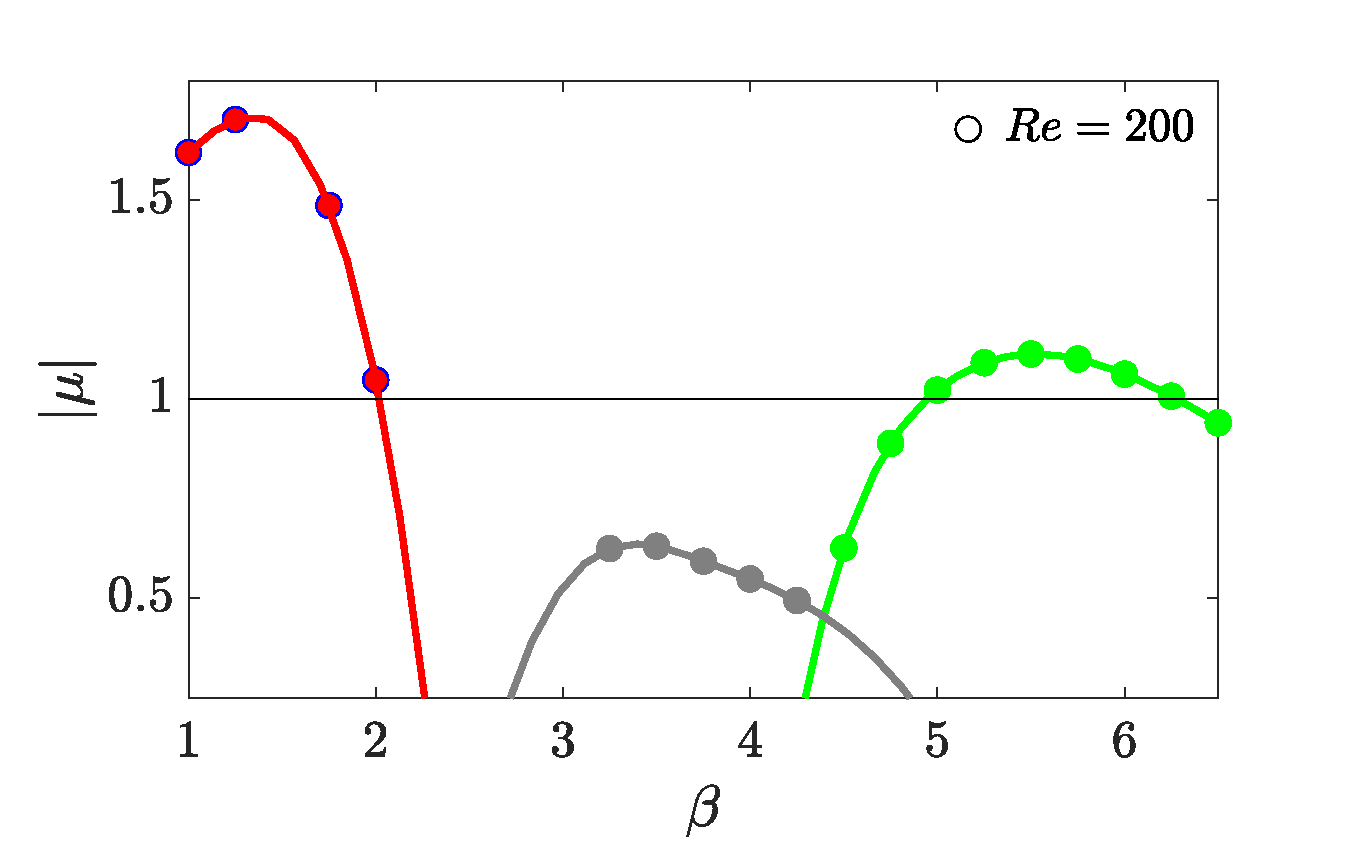
\includegraphics[width=0.49\textwidth]{./fig/AR1s/multipliers_AR1.eps}
  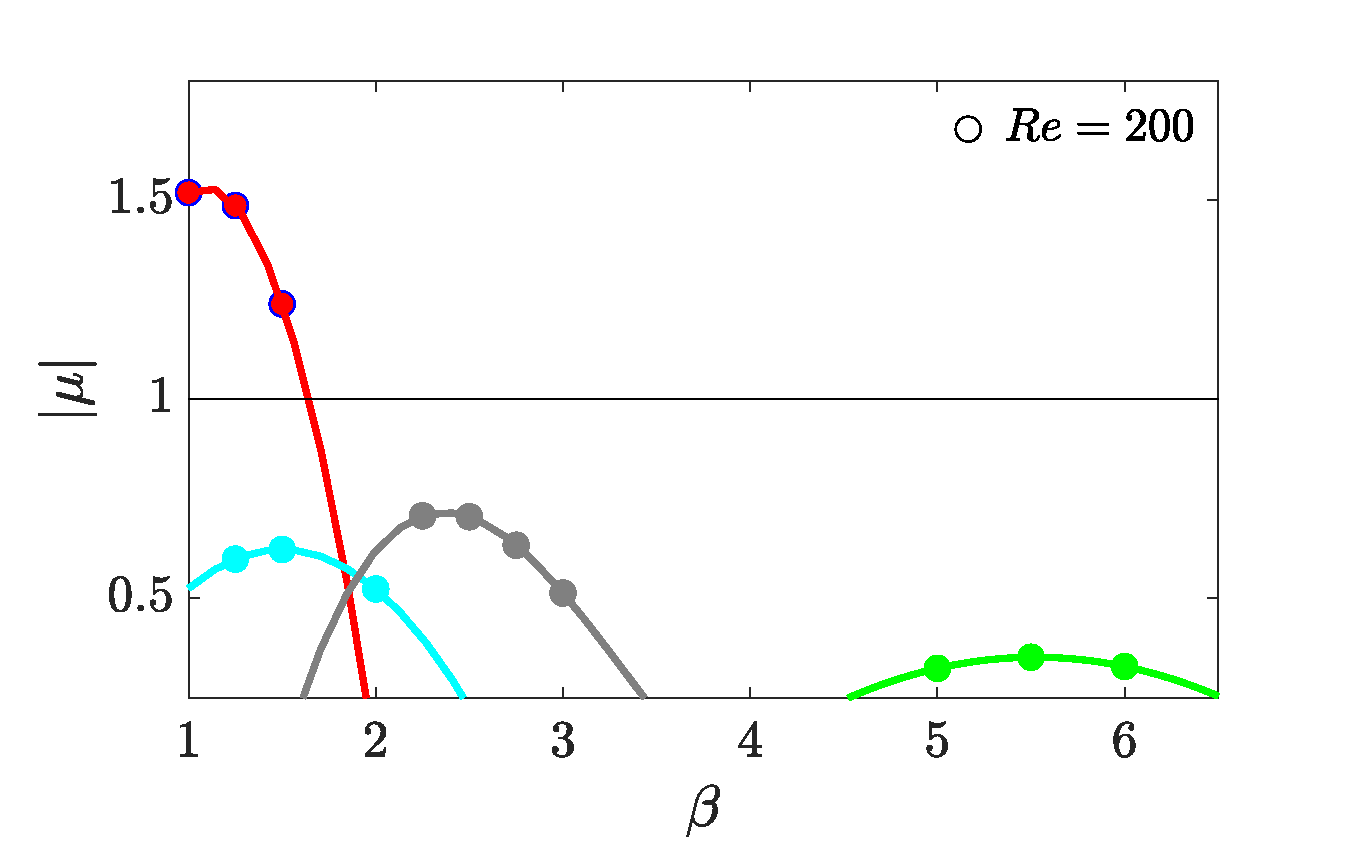
\includegraphics[width=0.49\textwidth]{./fig/AR1s/multipliers_AR1p25.eps}
  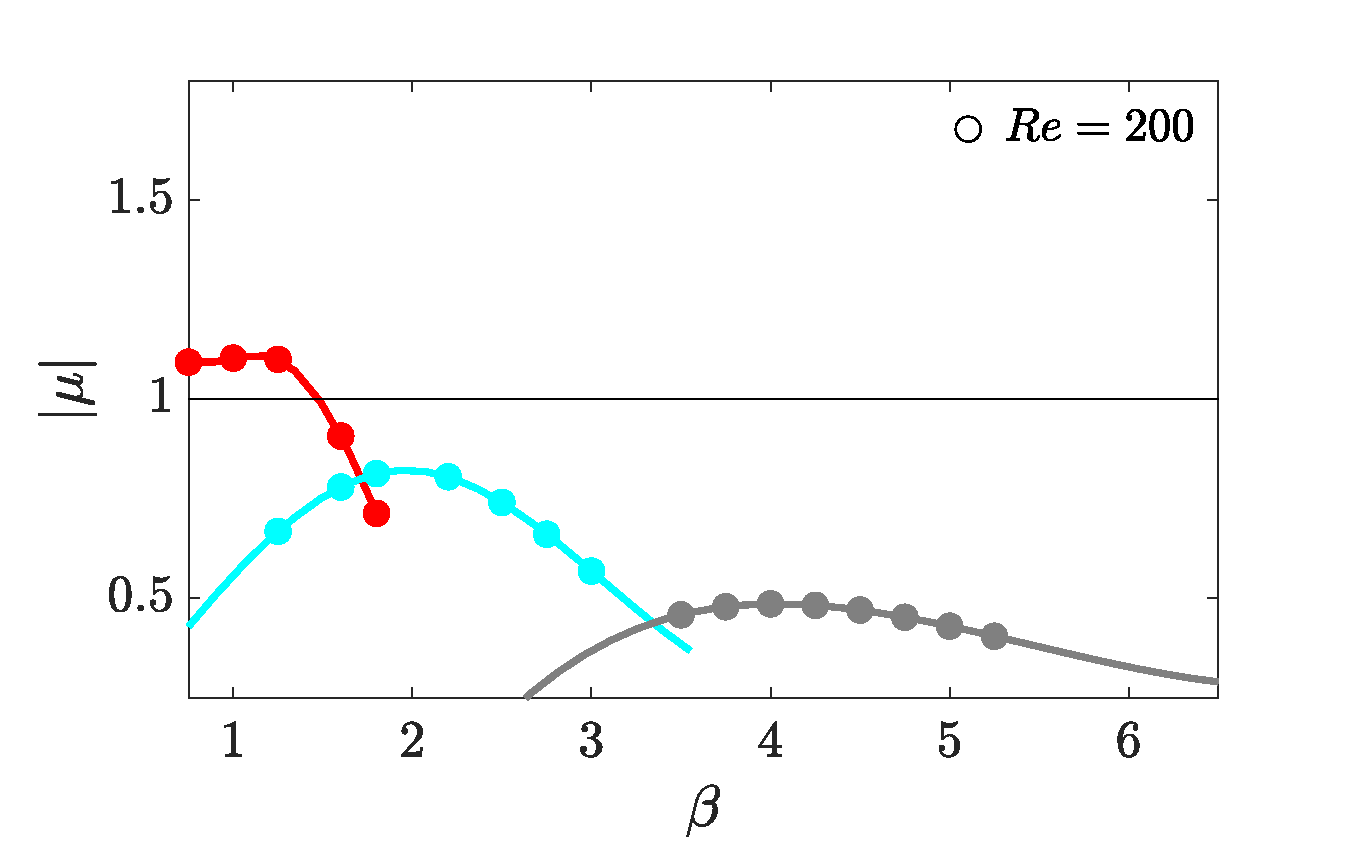
\includegraphics[width=0.49\textwidth]{./fig/AR1s/multipliers_AR1p5.eps}
  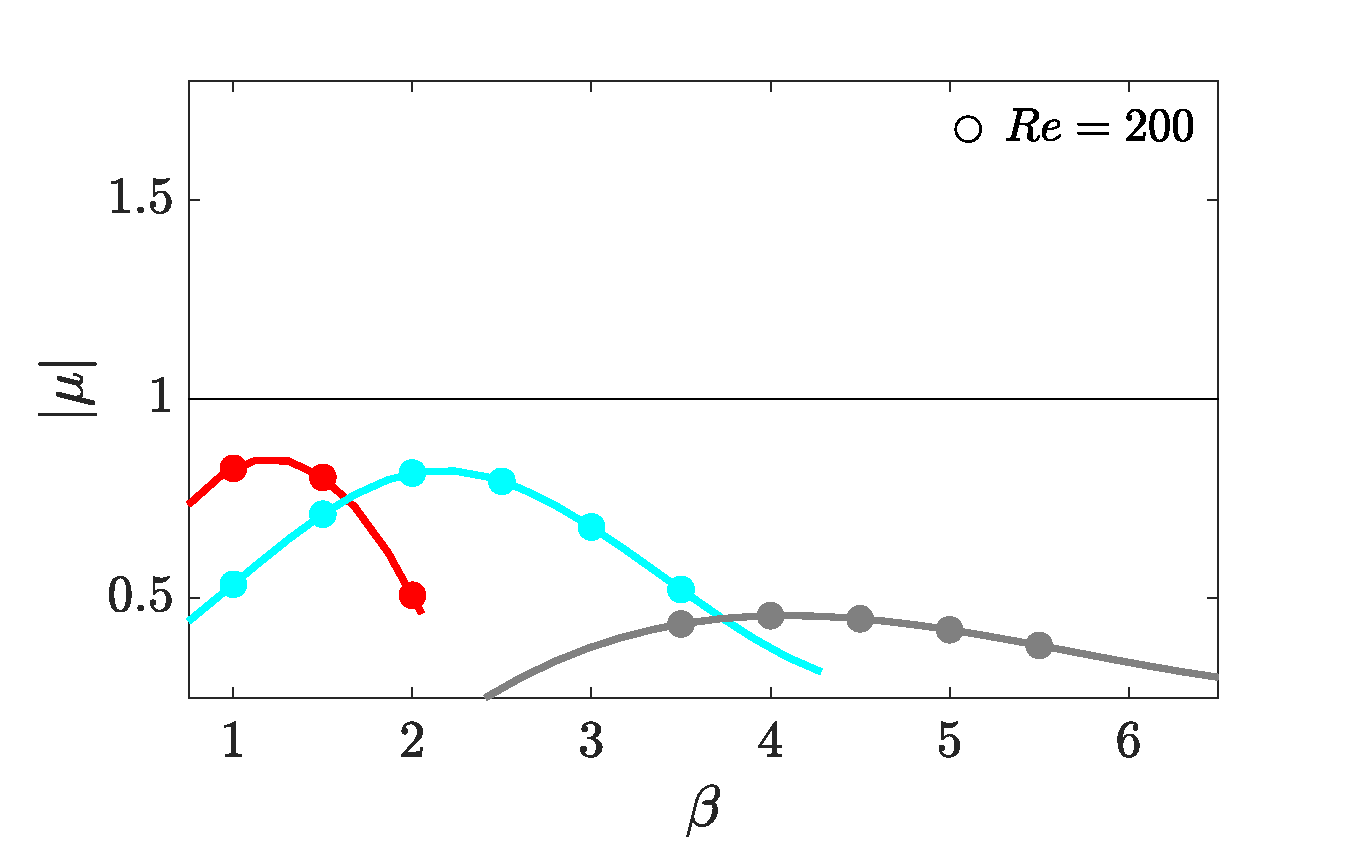
\includegraphics[width=0.49\textwidth]{./fig/AR1s/multipliers_AR1p75.eps} \\
  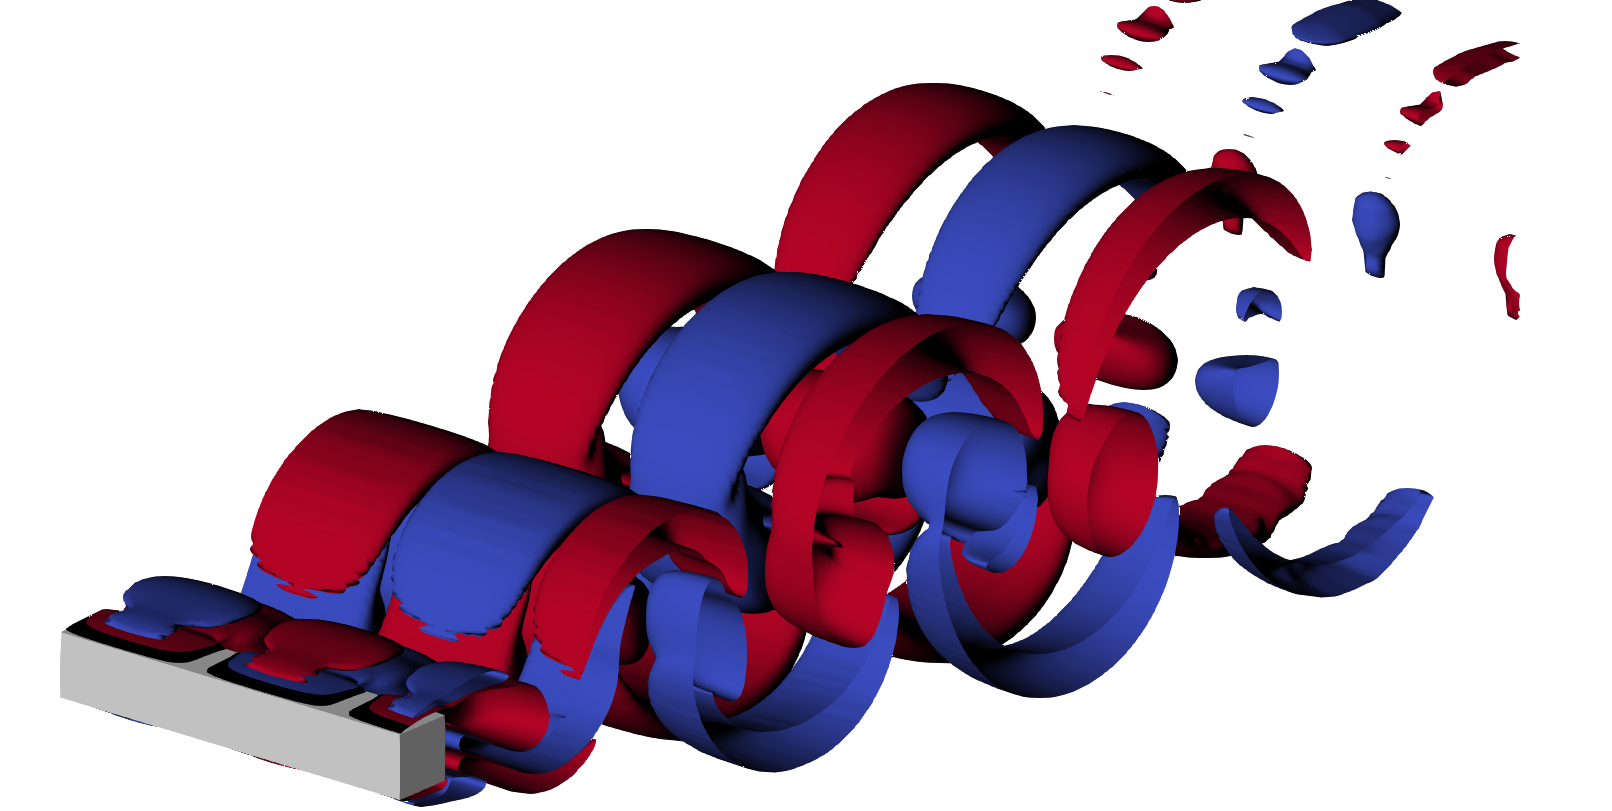
\includegraphics[width=0.32\textwidth]{./fig/AR1s/Floqetmode_beta_1p2_Re200_AR1_A.png}
  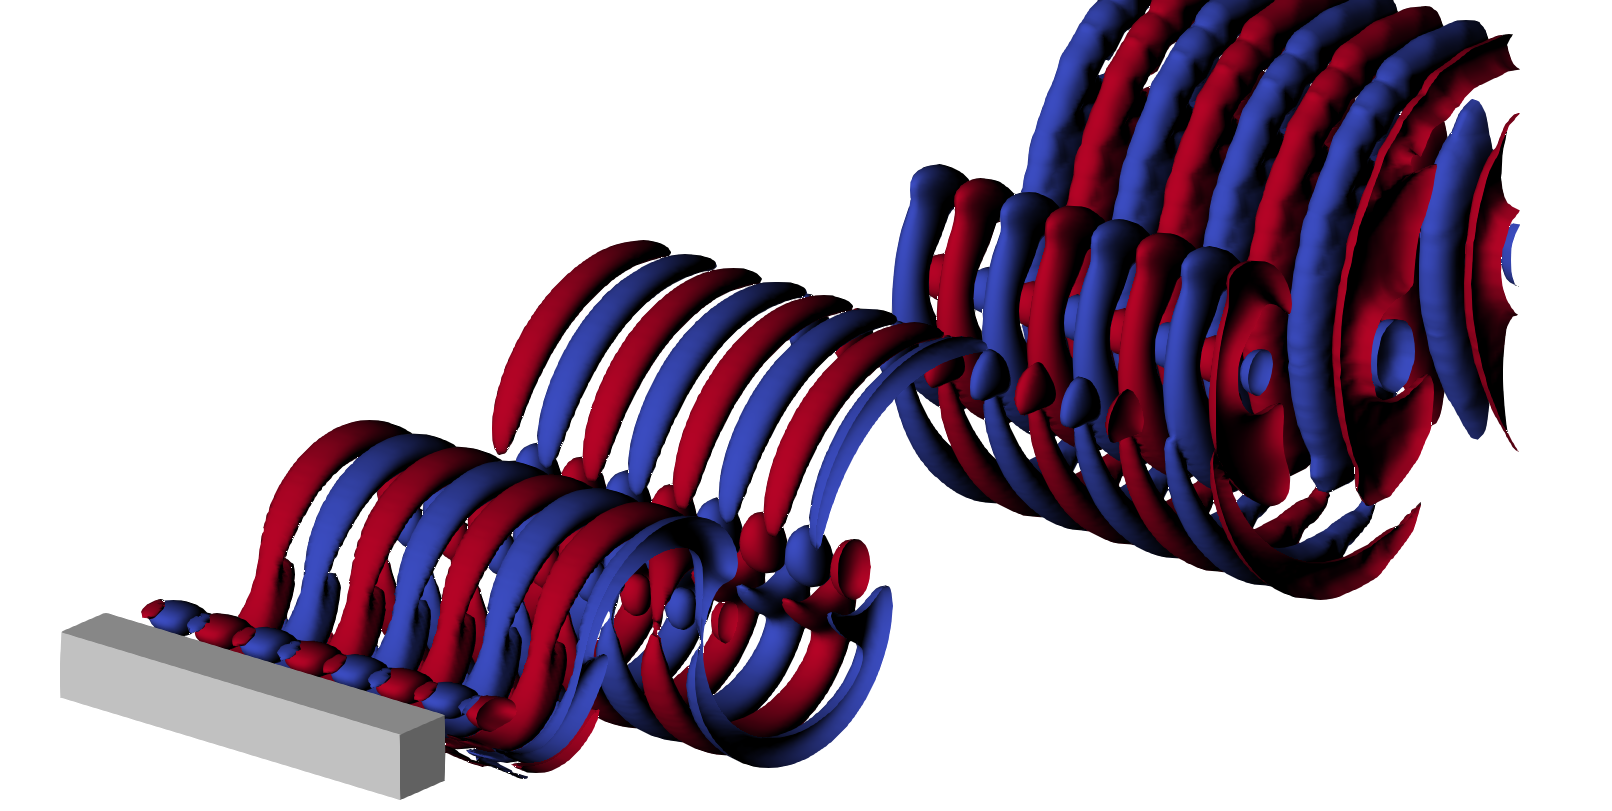
\includegraphics[width=0.32\textwidth]{./fig/AR1s/Floqetmode_beta_3p75_Re200_AR1_C.png}      
  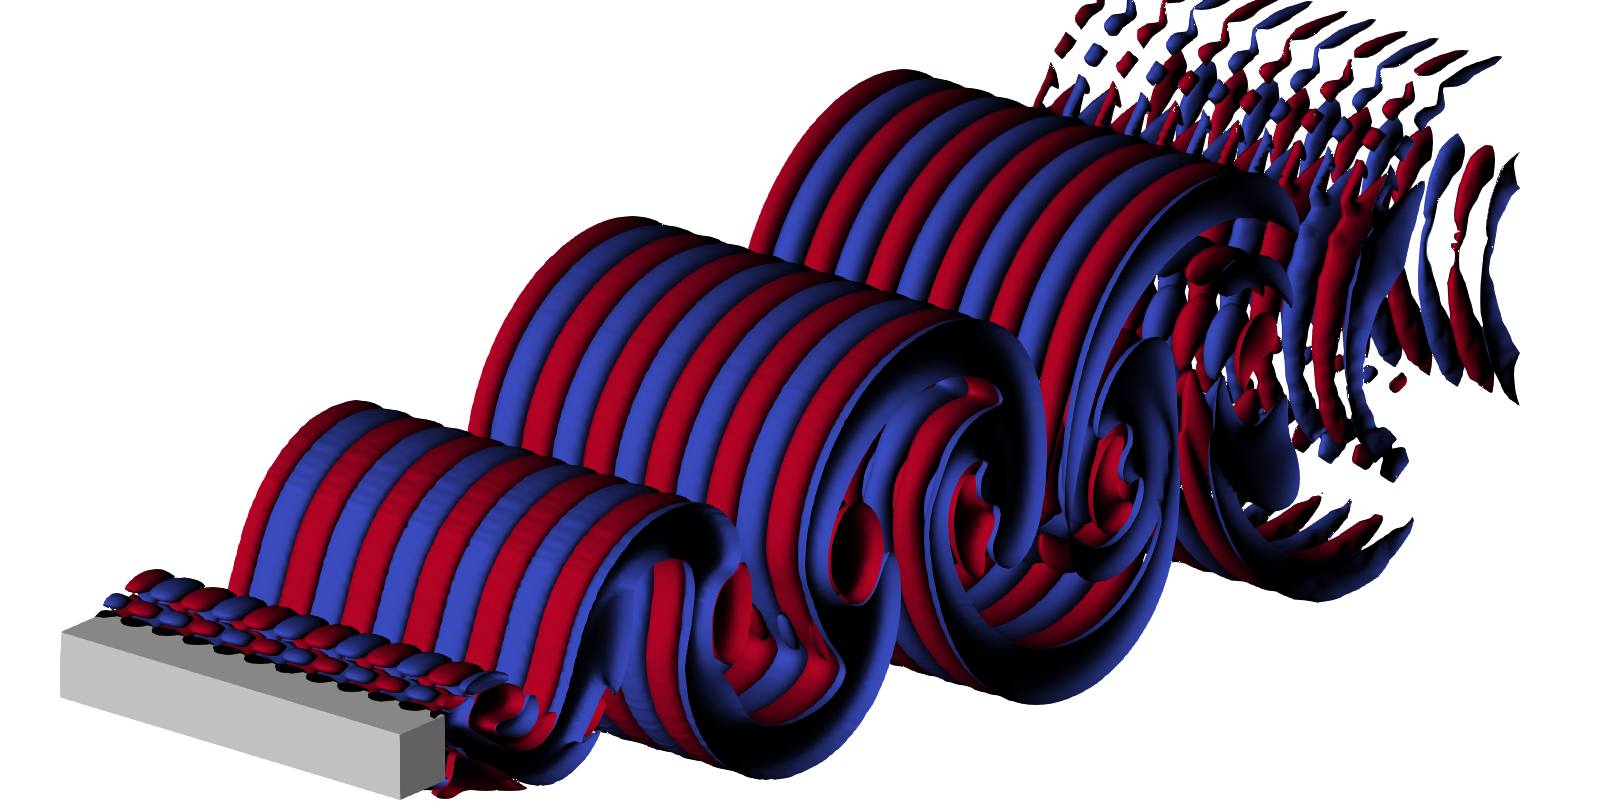
\includegraphics[width=0.32\textwidth]{./fig/AR1s/Floqetmode_beta_5p5_Re200_AR1_B.png}
  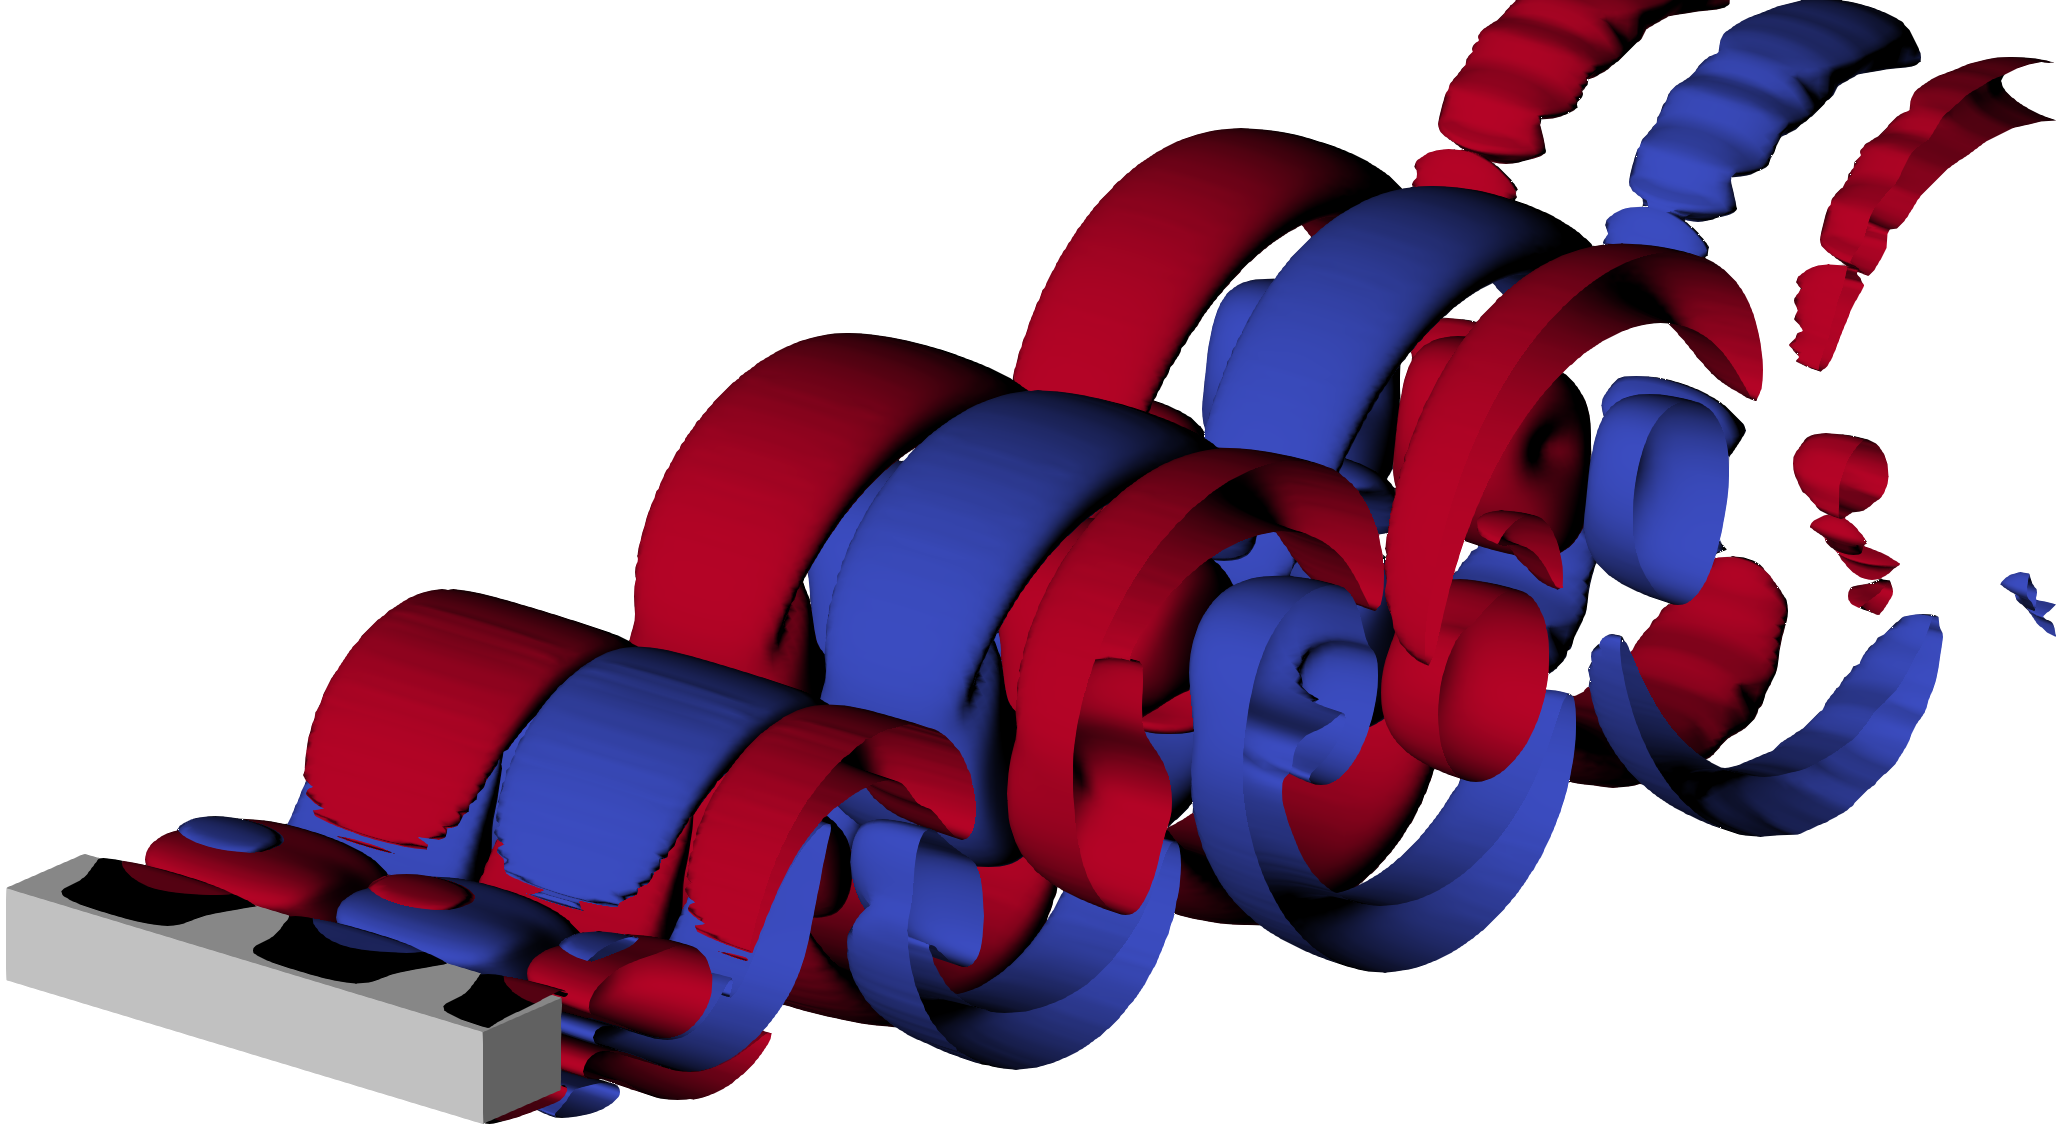
\includegraphics[width=0.32\textwidth]{./fig/AR1s/Floqetmode_beta_1p25_Re200_AR1p25_A.png}
  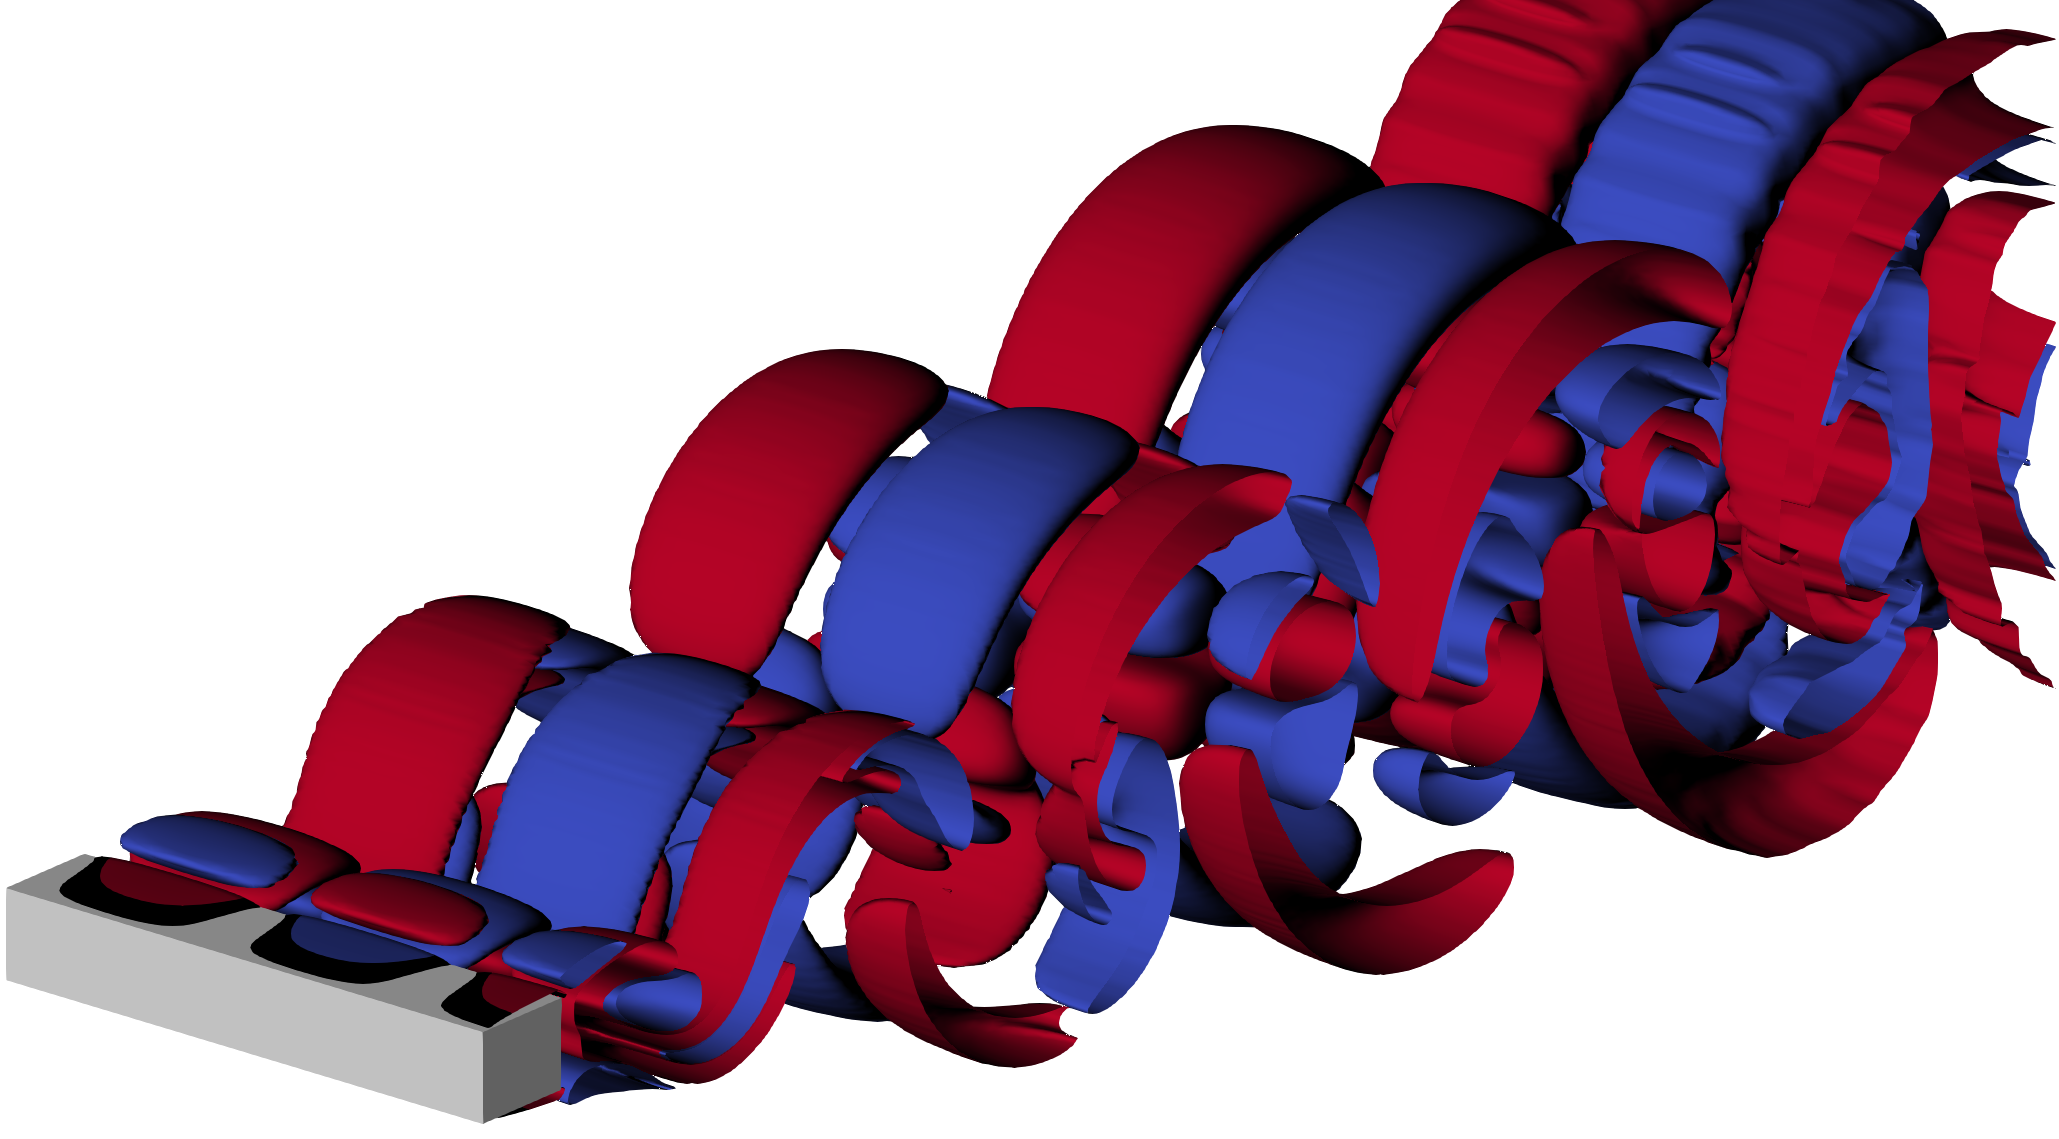
\includegraphics[width=0.32\textwidth]{./fig/AR1s/Floqetmode_beta_1p25_Re200_AR1p25_Bp.png}
  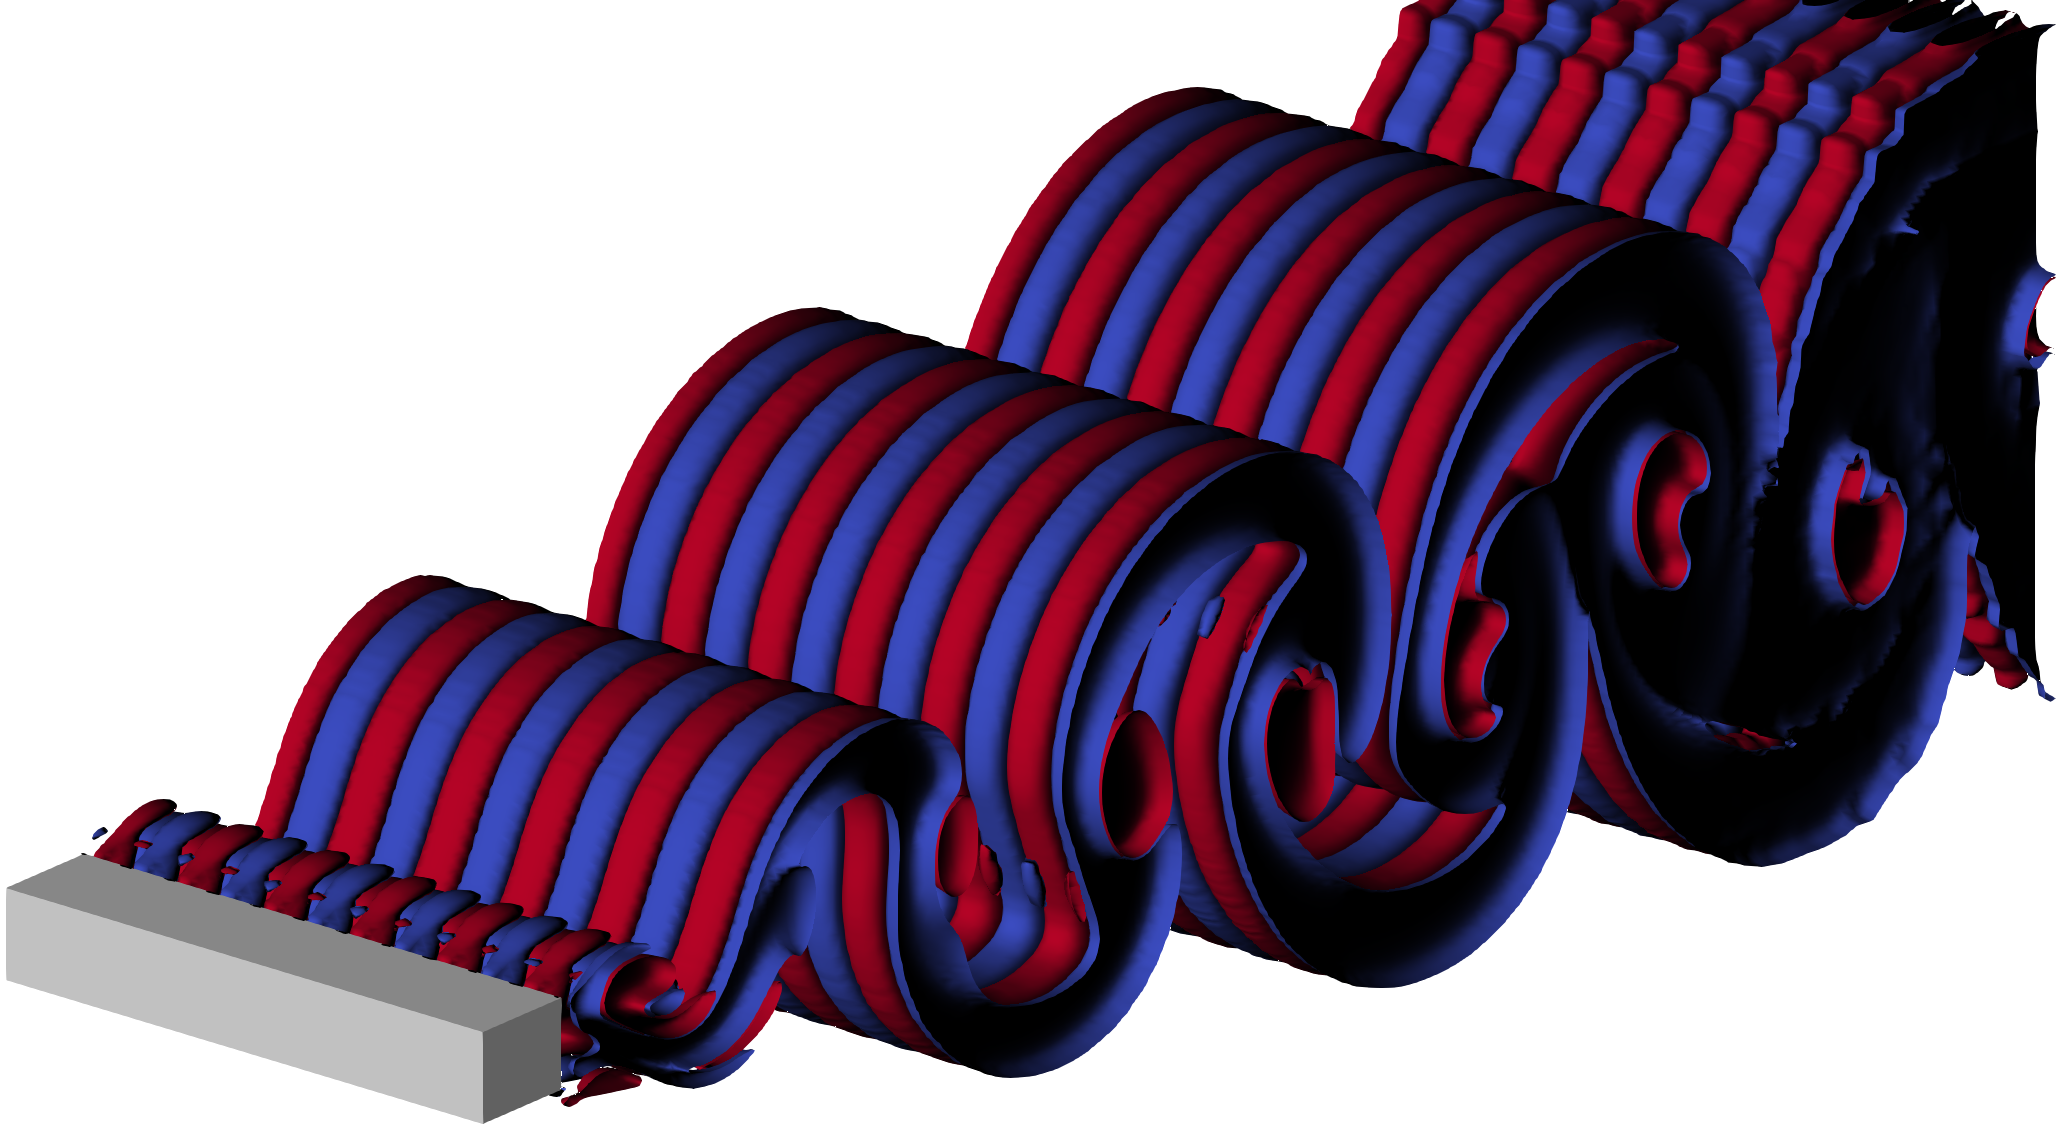
\includegraphics[width=0.32\textwidth]{./fig/AR1s/Floqetmode_beta_5p5_Re200_AR1p25_B.png}
  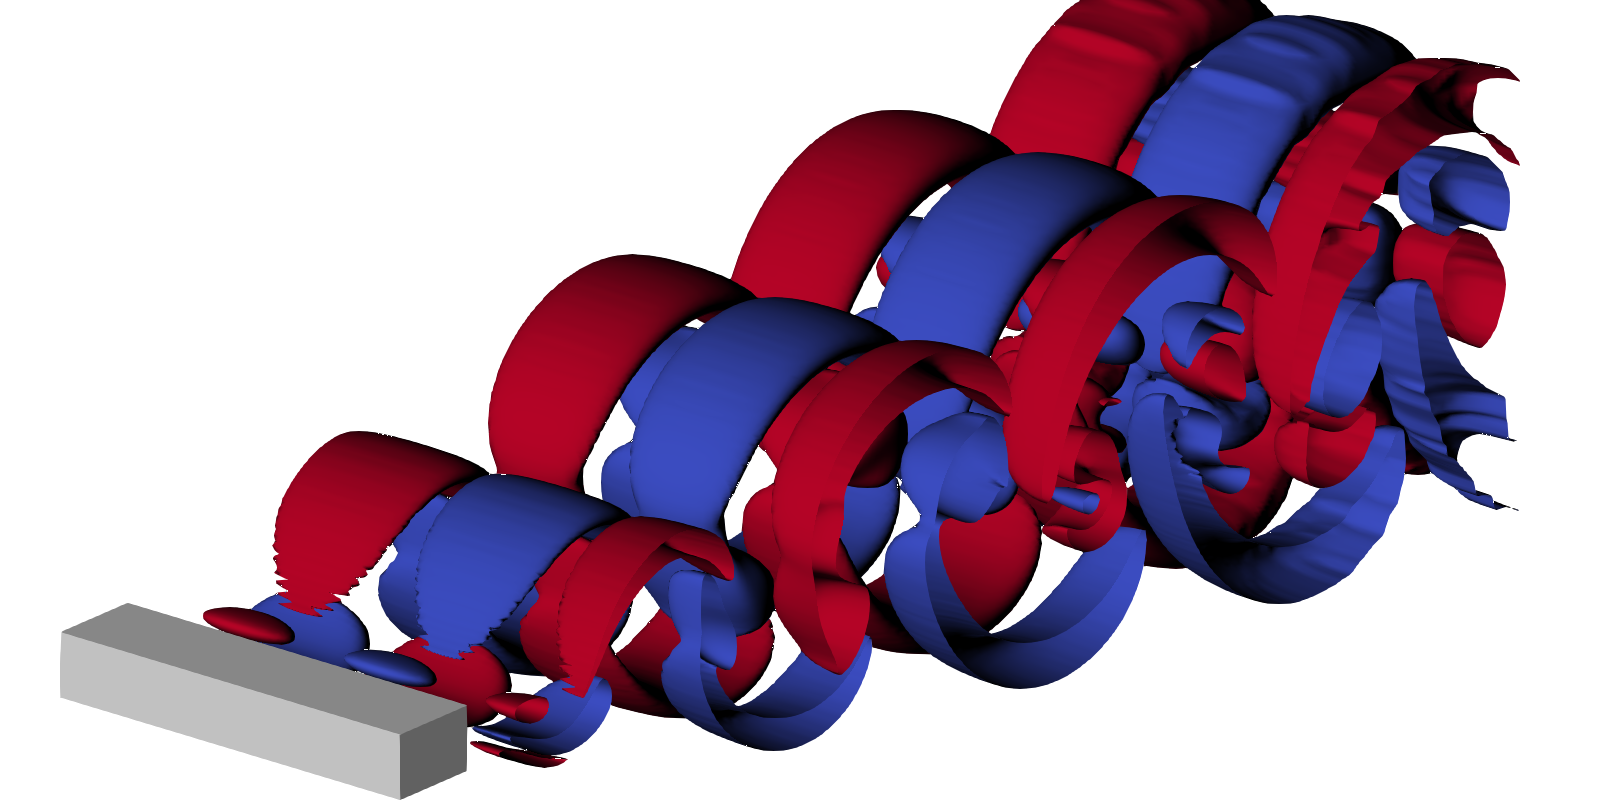
\includegraphics[width=0.32\textwidth]{./fig/AR1s/Floqetmode_beta_1p8_Re200_AR1p5_A.png}
  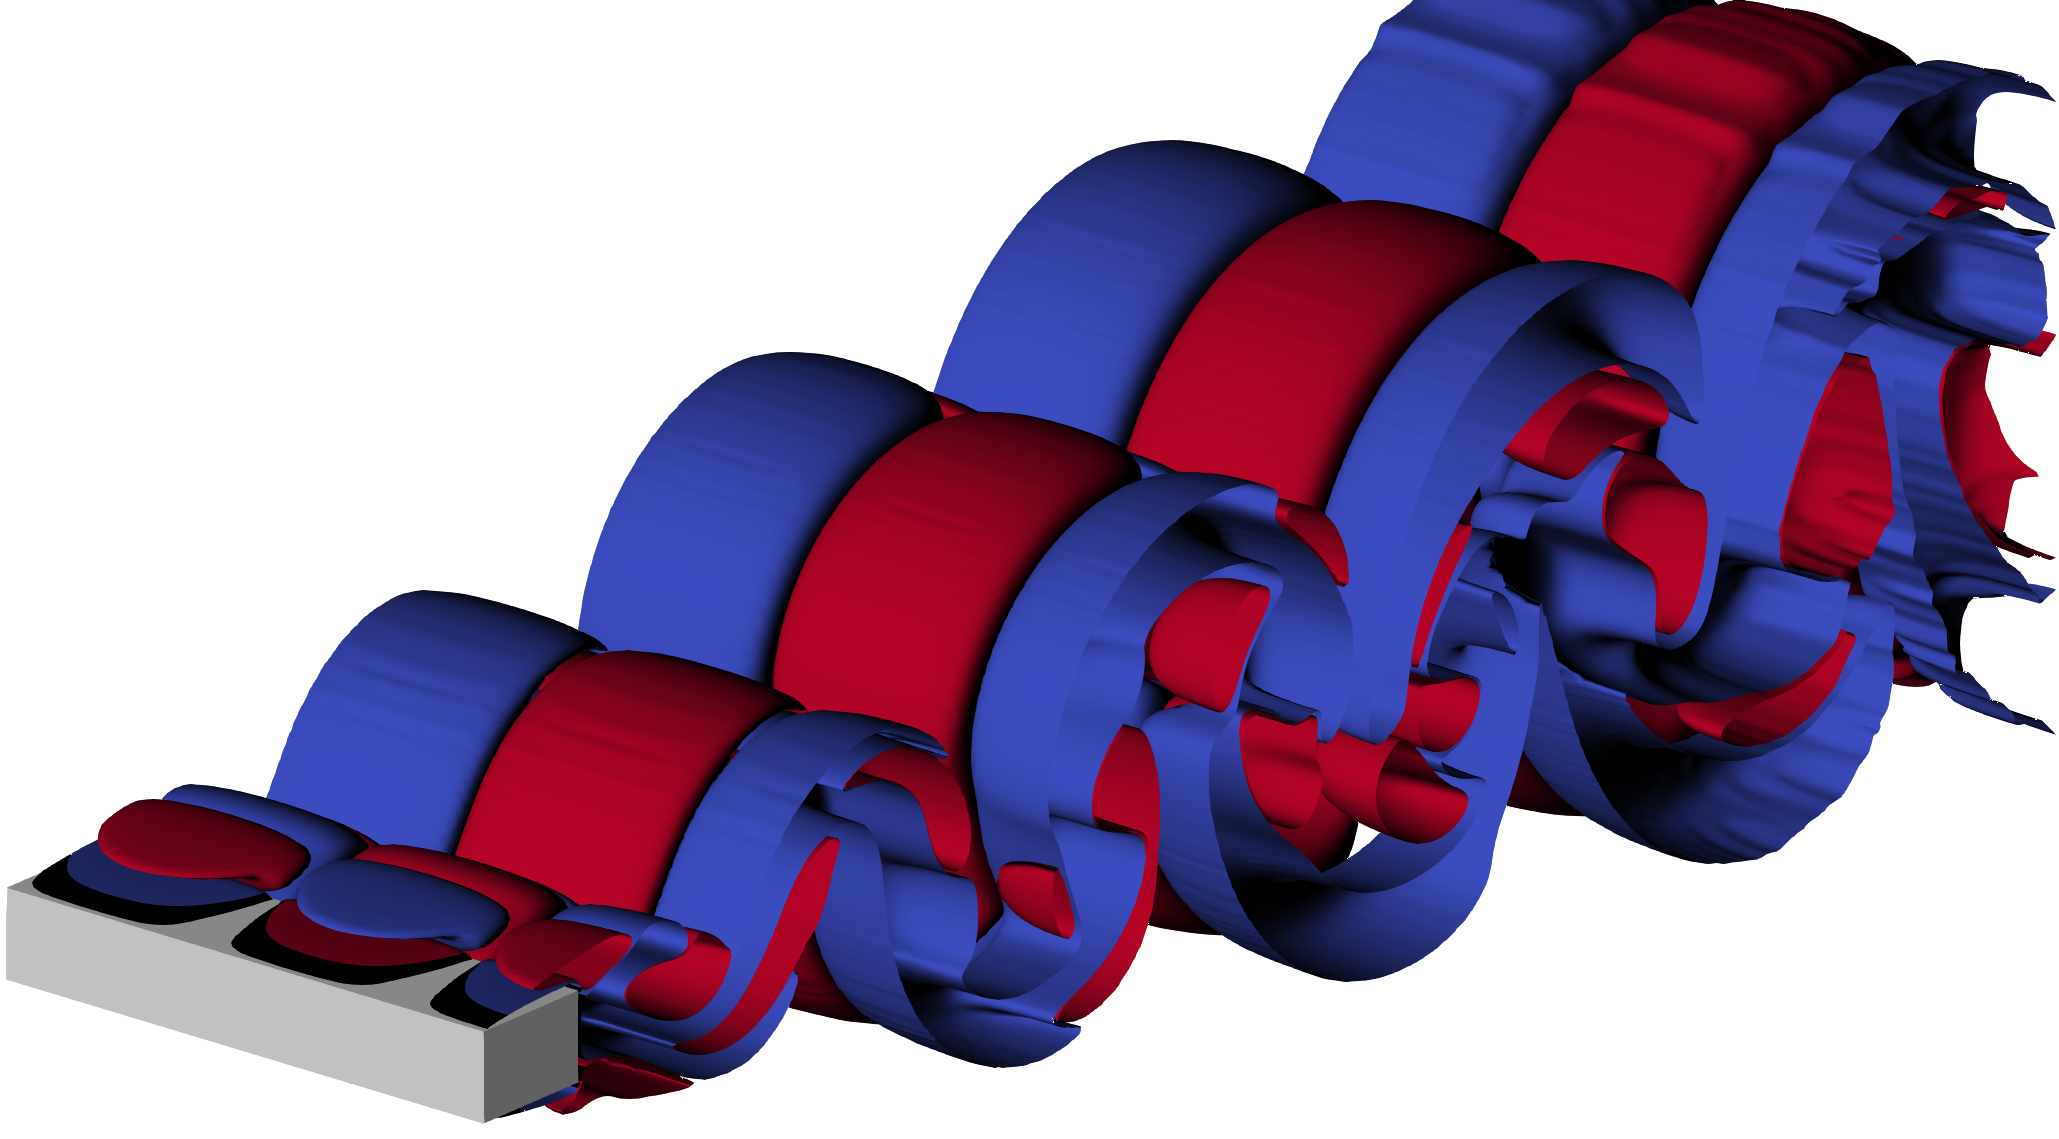
\includegraphics[width=0.32\textwidth]{./fig/AR1s/Floqetmode_beta_1p8_Re200_AR1p5_Bp.png}
  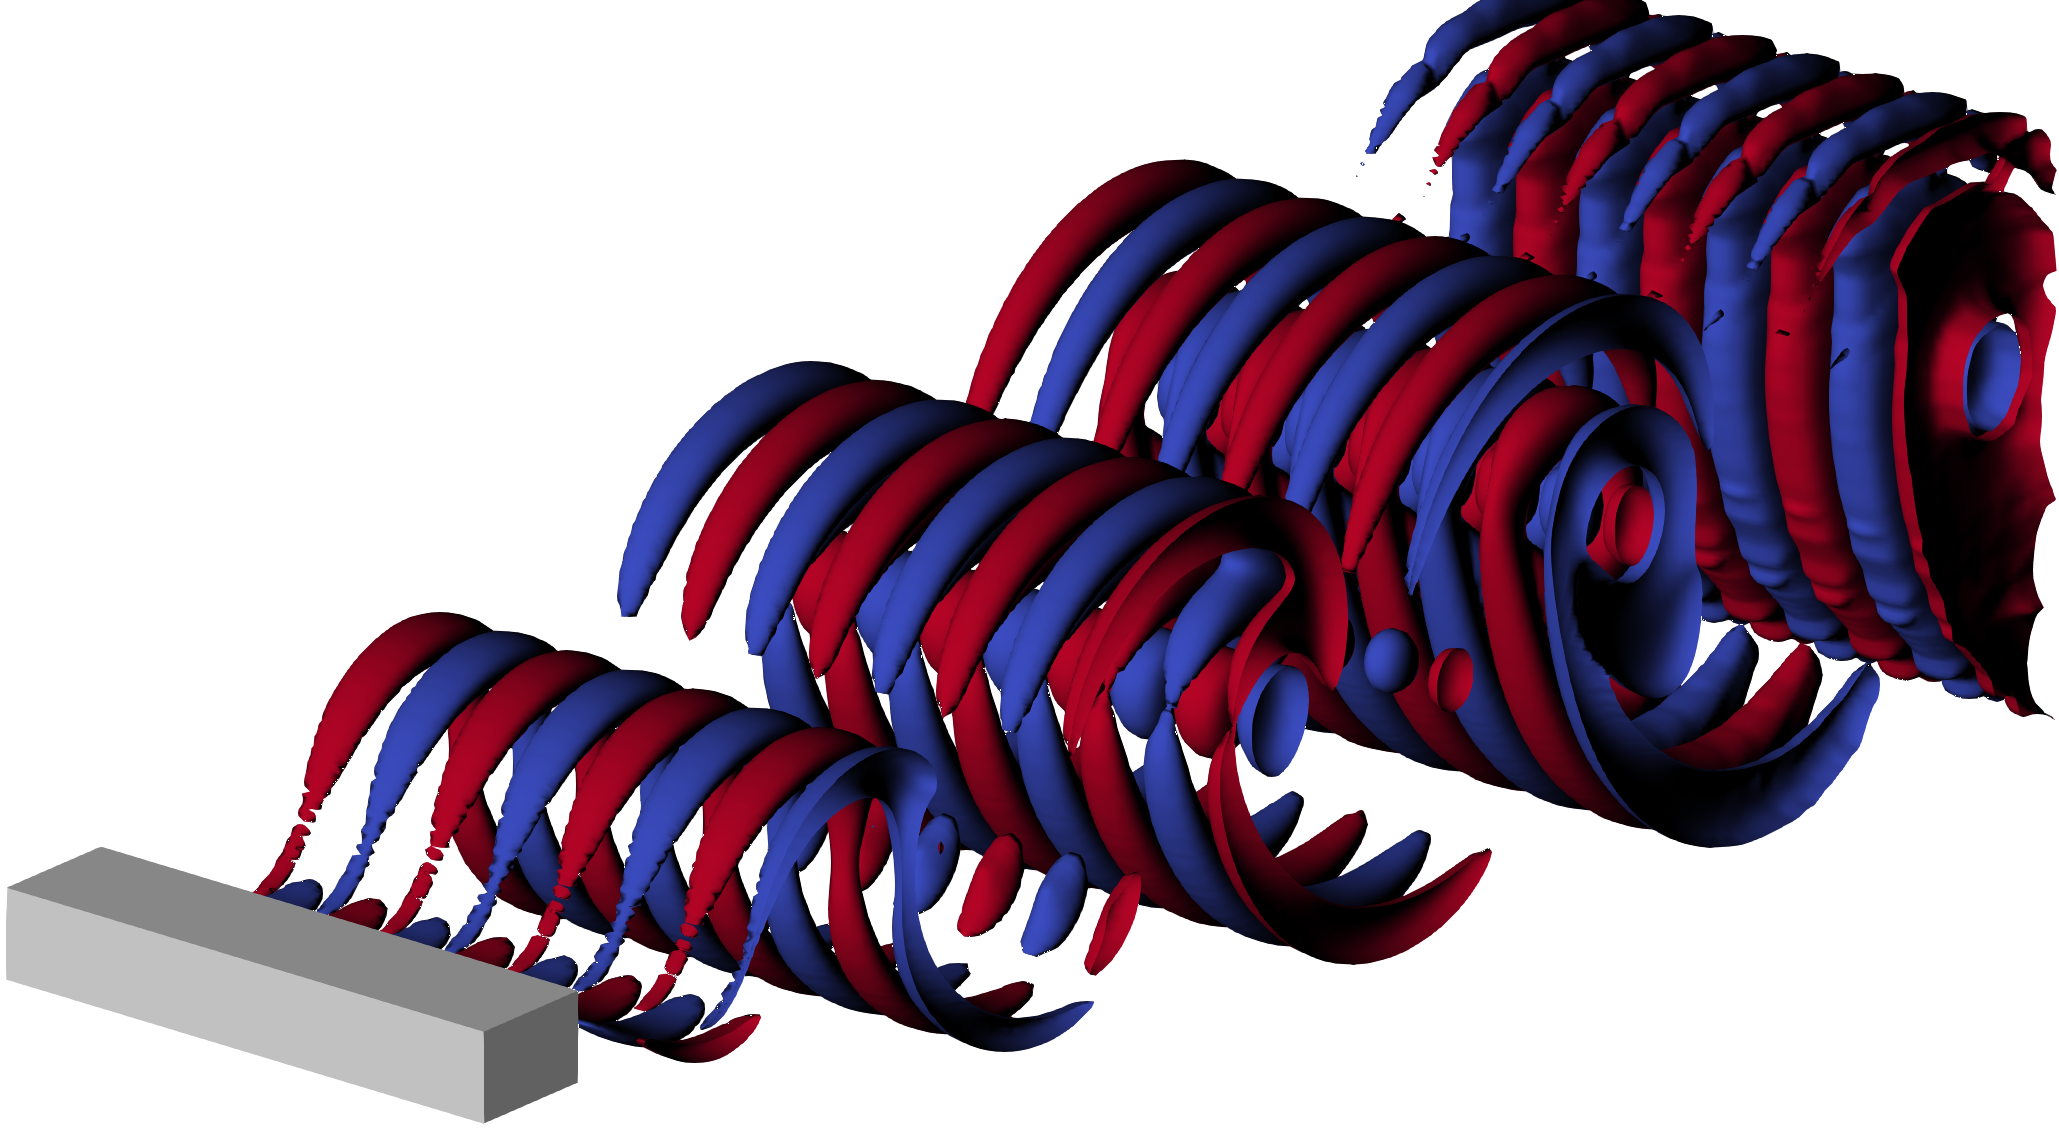
\includegraphics[width=0.32\textwidth]{./fig/AR1s/Floqetmode_beta_3p75_Re200_AR1p5_C.png}
  \caption{Top: multipliers for $\AR=1$, $\AR=1.25$ and $\AR=1.5$ at $Re=200$; the red line refers to mode $A$, the grey line to mode $C$, the green line to mode $B$ and the light blue line refers to mode $B'$. Mode $B'$ has the same spatio-temporal symmetry of mode $B$, but its characteristic wavelength is much smaller, being similar to that of mode $A$. This mode resembles that found for elongated bodies with elliptic leading edge by \cite{ryan-etal-2005}. The bottom panels show the Floquet modes associated with the different branches for the three $\AR$s. Top: Floquet modes for $\AR=1$ and $Re=200$, associated with mode A (left, $\beta=1.2$), mode C (centre, $\beta=3.75$) and mode $B$ (right, $\beta=5.5$). Centre: Floquet modes for $\AR=1.25$ and $Re=200$ associated with mode A (left, $\beta=1.25$), mode $B'$ (centre, $\beta = 1.25$) and mode $B$ (right, $\beta=5.5$). Bottom: Floquet modes for $\AR=1.5$ and $Re=200$ associated with mode A (left, $\beta=1.8$), mode $B'$ (centre, $\beta=1.8$) and mode $C$ (right, $\beta=3.75$). These are 3D reconstructions of the Floquet modes and the red/blue isosurfaces denote positive/negative streamwise vorticity.}
  \label{fig:xx}
\end{figure}


\begin{figure}
  \centering
  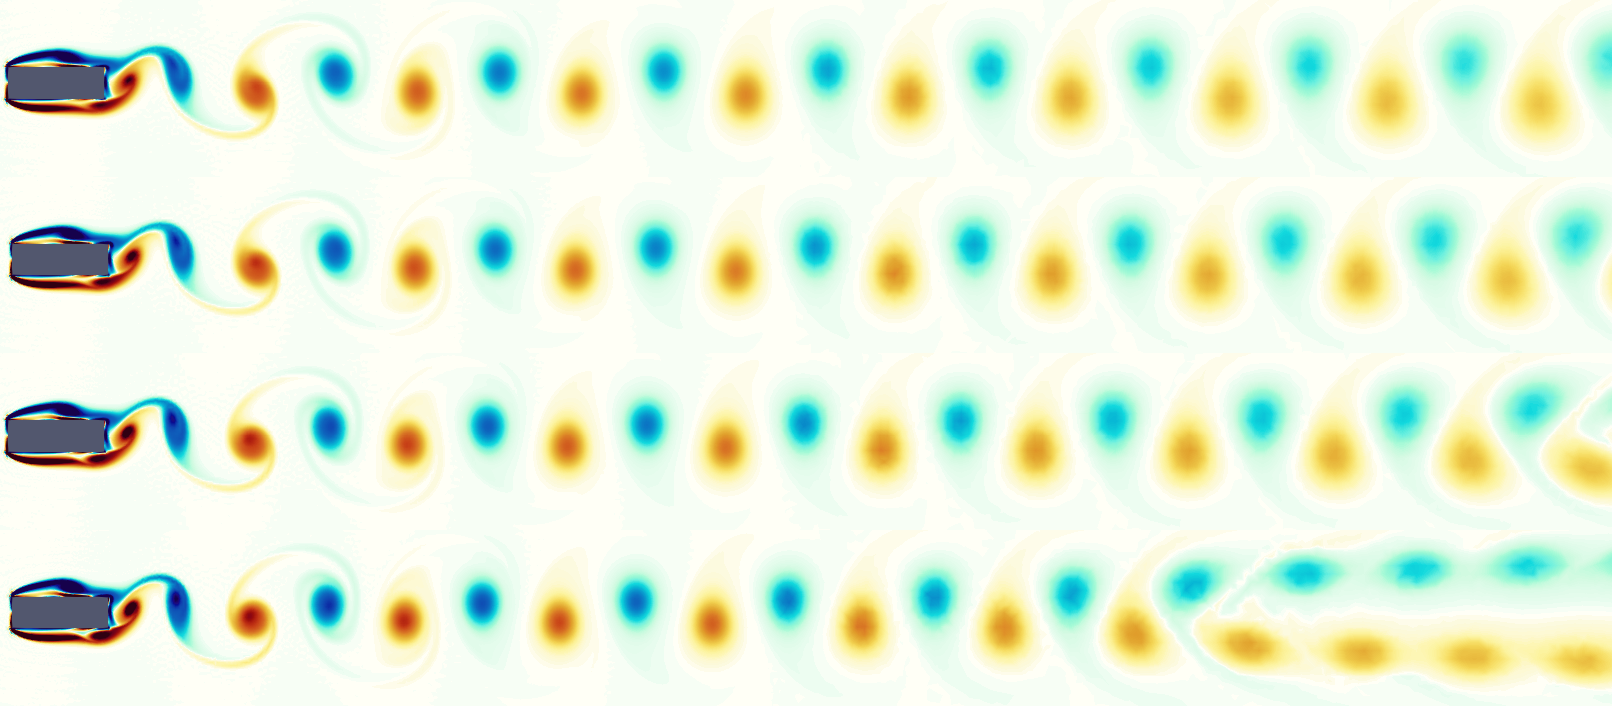
\includegraphics[width=0.8\textwidth]{./fig/AR3/BF_vort_Re400_475.png}
  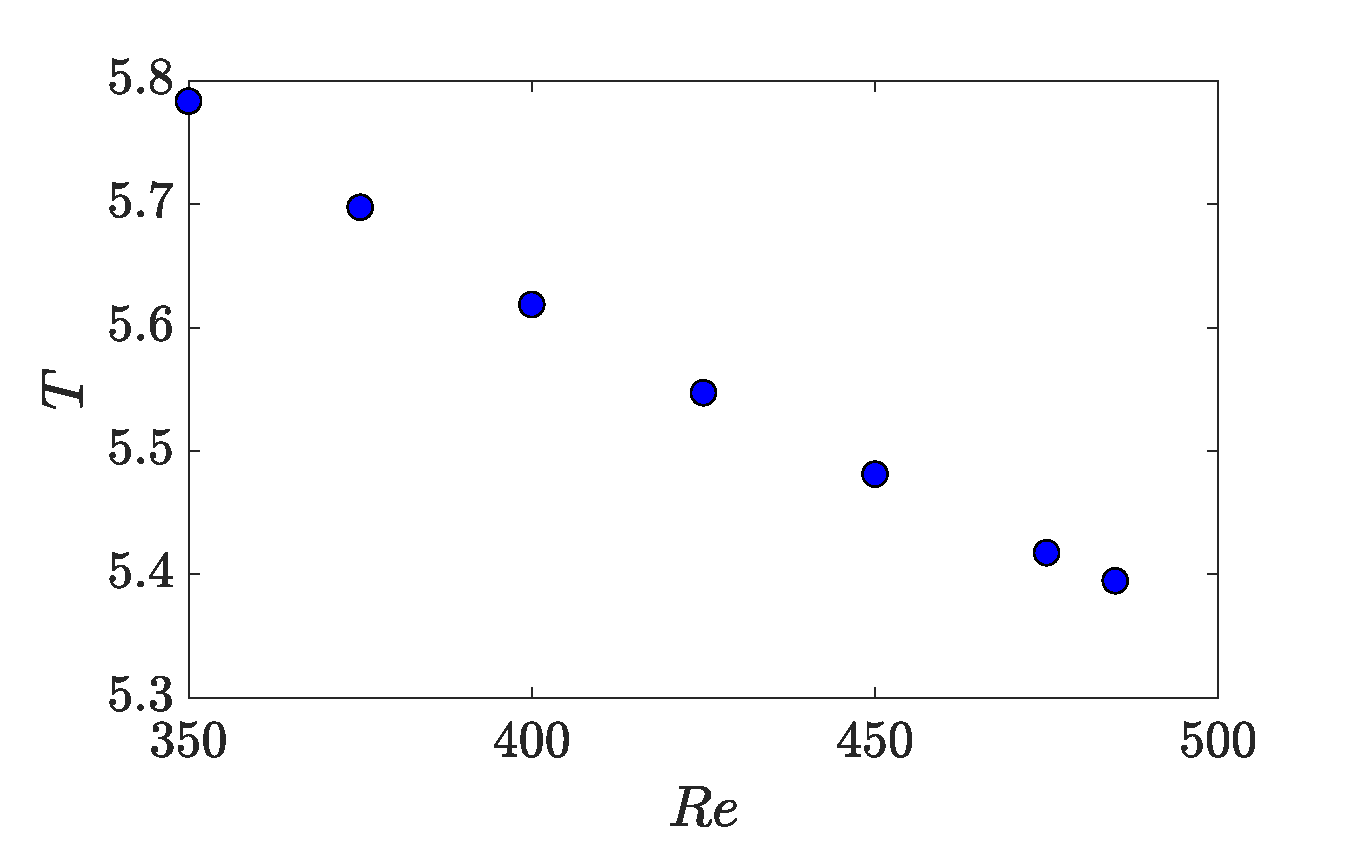
\includegraphics[width=0.5\textwidth]{./fig/AR3/T_Re.eps}
  \caption{Base flow vorticity snapshots for $\AR=3$ at (from top to bottom) $Re=400$, $Re=425$, $Re=450$ and $Re=485$. Note that as $Re$ increases the structure of the wake changes, with the positive and negative vorticity monopoles being clearly separated. As $Re$ increases, this separation start occurring closer to the TE. Bottom panel: Dependence of the period $T$ on $Re$ for the periodic regime in the $350 \le Re \le 485$ range.}
  \label{fig:BF_AR3}
\end{figure}

\begin{figure}
  \centering
  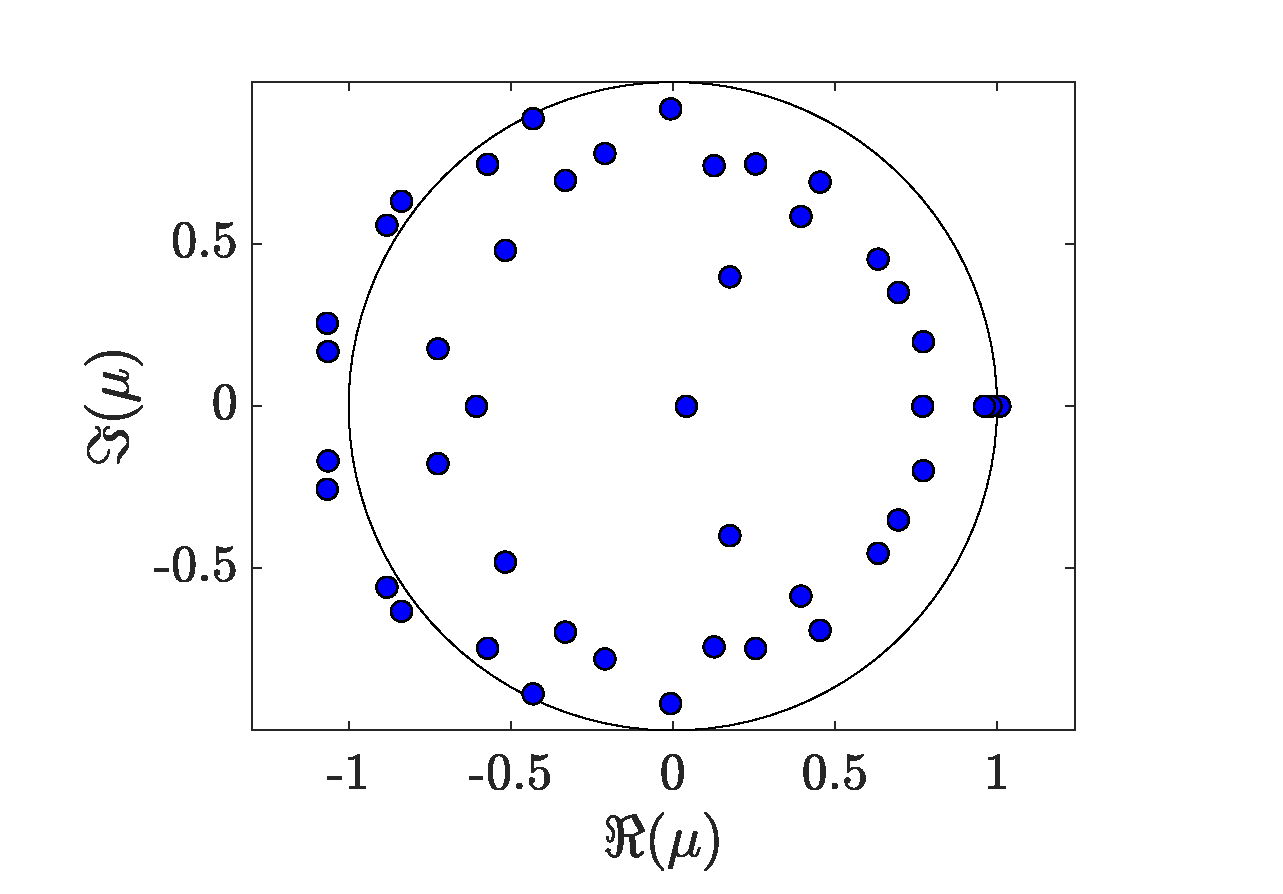
\includegraphics[width=0.5\textwidth]{./fig/AR3/mult_Re495_beta0.eps}
  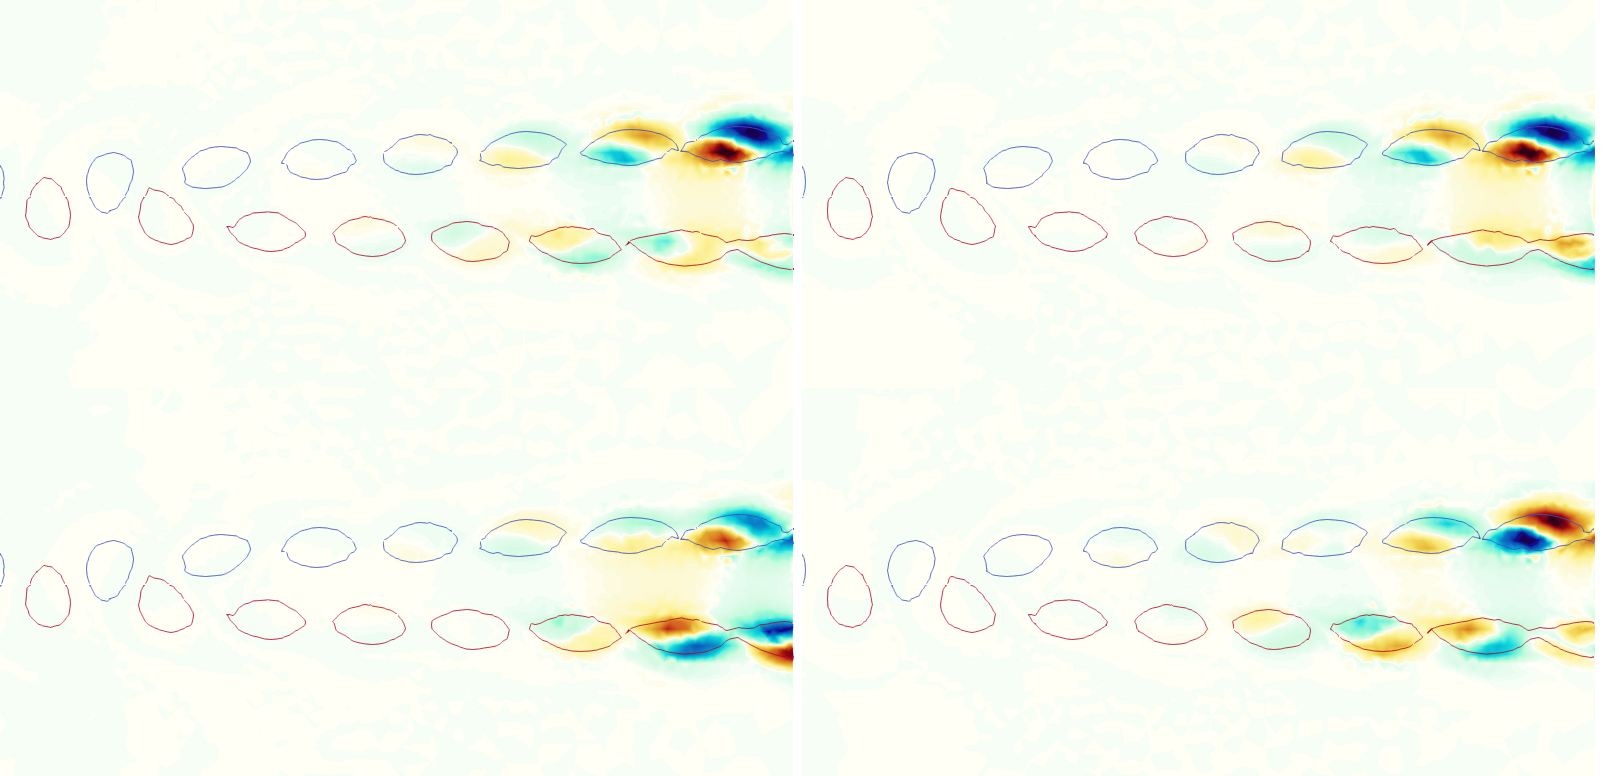
\includegraphics[width=1.0\textwidth]{./fig/AR3/Floquet_modes_beta_0_Re495.png}
  \caption{Floquet analysis for $\AR=3$ and $Re=495$. Top: Floquet multilpiers for $\beta = 0$. Bottom: Modes associated with the $4$ multipliers outside the unit circumference.}
  \label{fig:AR3_Stab}
\end{figure}


\begin{itemize}
  \item Start from $\AR=1$ and investigate what happens for $1 \le \AR \le 2$. How does the $\AR$ influence mode $A$, mode $B$ and $QS$? This is the easy part, I expect that some modes become more stable, while other less stable {\color{red} Floquet analysis here needs to be redone}
  \item For $\AR=3$ we observe that mode $A$ is apparently stable. However, as we increase the Reynolds number the structure of the far wake changes, with the monopoles of positive and negative vorticity being separated (see figure \ref{fig:BF_AR3}). As shown in the bottom panel of figure \ref{fig:BF_AR3}, this occurs without a change of the flow periodicity. {\color{red} I am currently investigating whether this is due to a synchronous global instability of the base flow. Also, I am performing Floquet stability analysis over different $Re$.}
\end{itemize}

\subsection{Intermediate bodies with $3 < \AR < 4.75$}


\begin{figure}
  \centering
  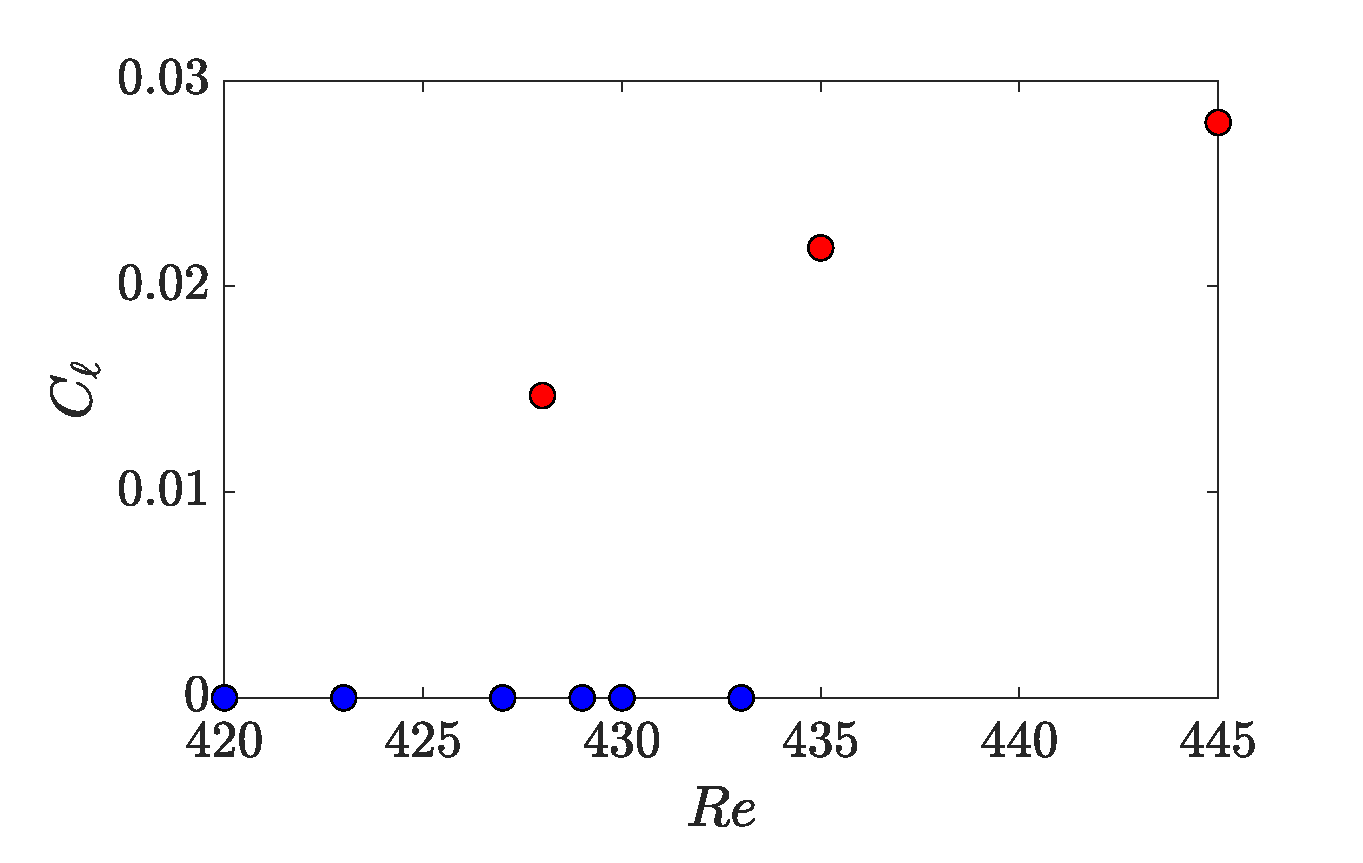
\includegraphics[width=0.49\textwidth]{./fig/AR4_Cl_Re.eps}
  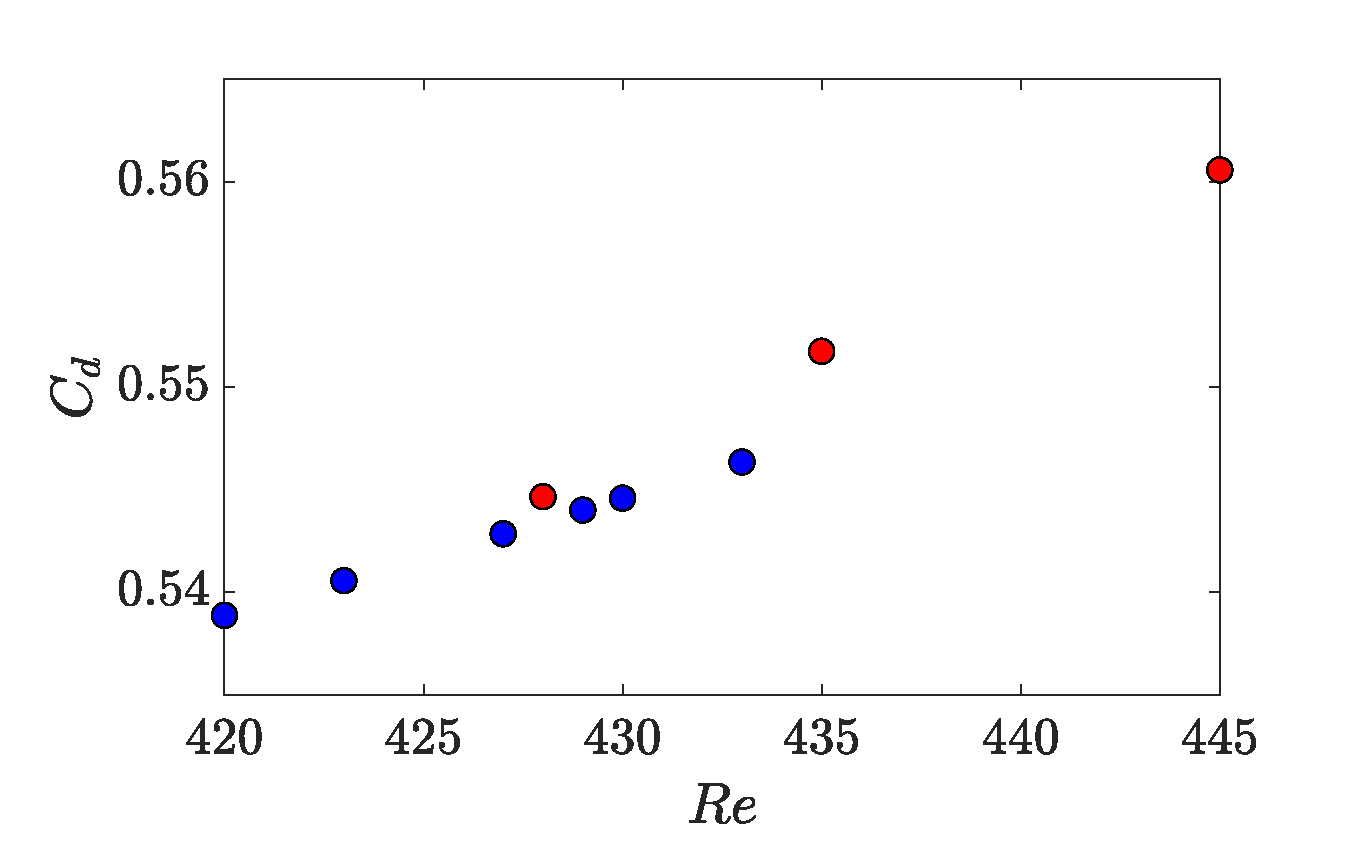
\includegraphics[width=0.49\textwidth]{./fig/AR4_Cd_Re.eps}
  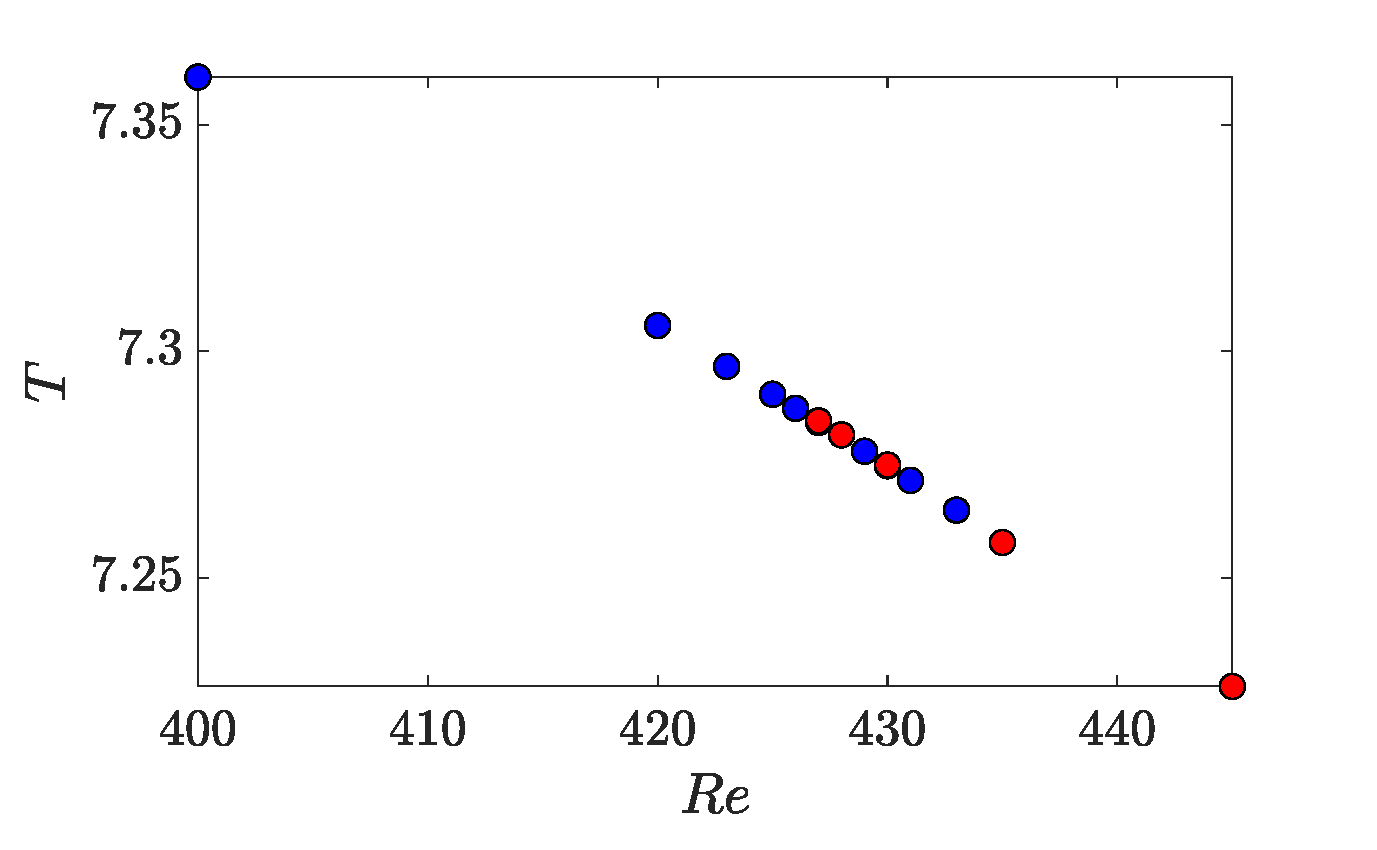
\includegraphics[width=0.49\textwidth]{./fig/AR4_T_Re.eps}
  \caption{Dependence of $C_\ell$, $C_d$ and $T$ on the Reynolds number $Re$.}
  \label{fig:Cl-Cd-AR4}
\end{figure}

\begin{figure}
\centering
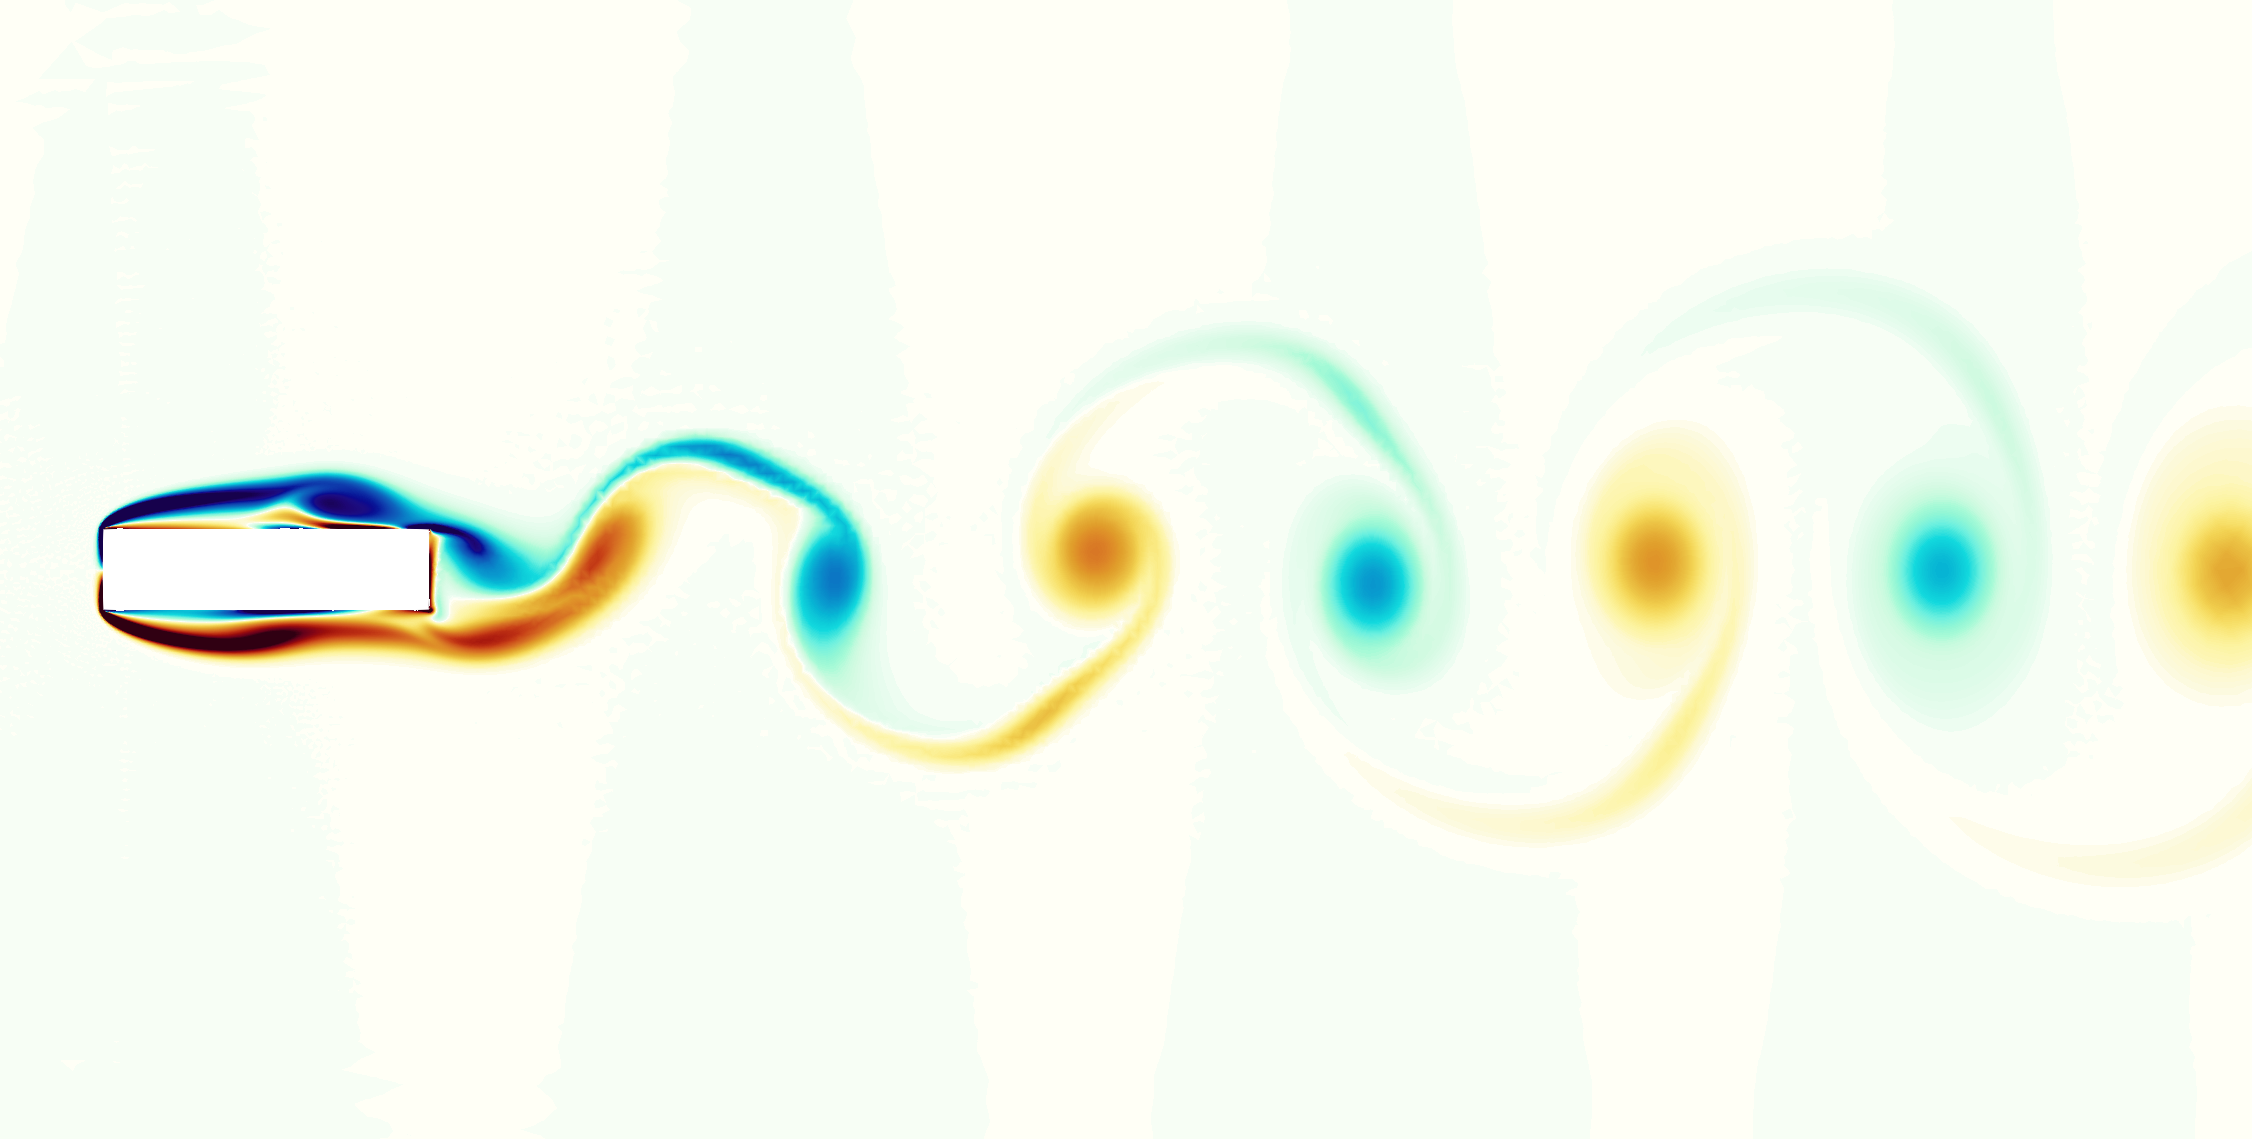
\includegraphics[trim={0 100 0 100},clip,width=0.49\textwidth]{./fig/vort_Re425_25.png}
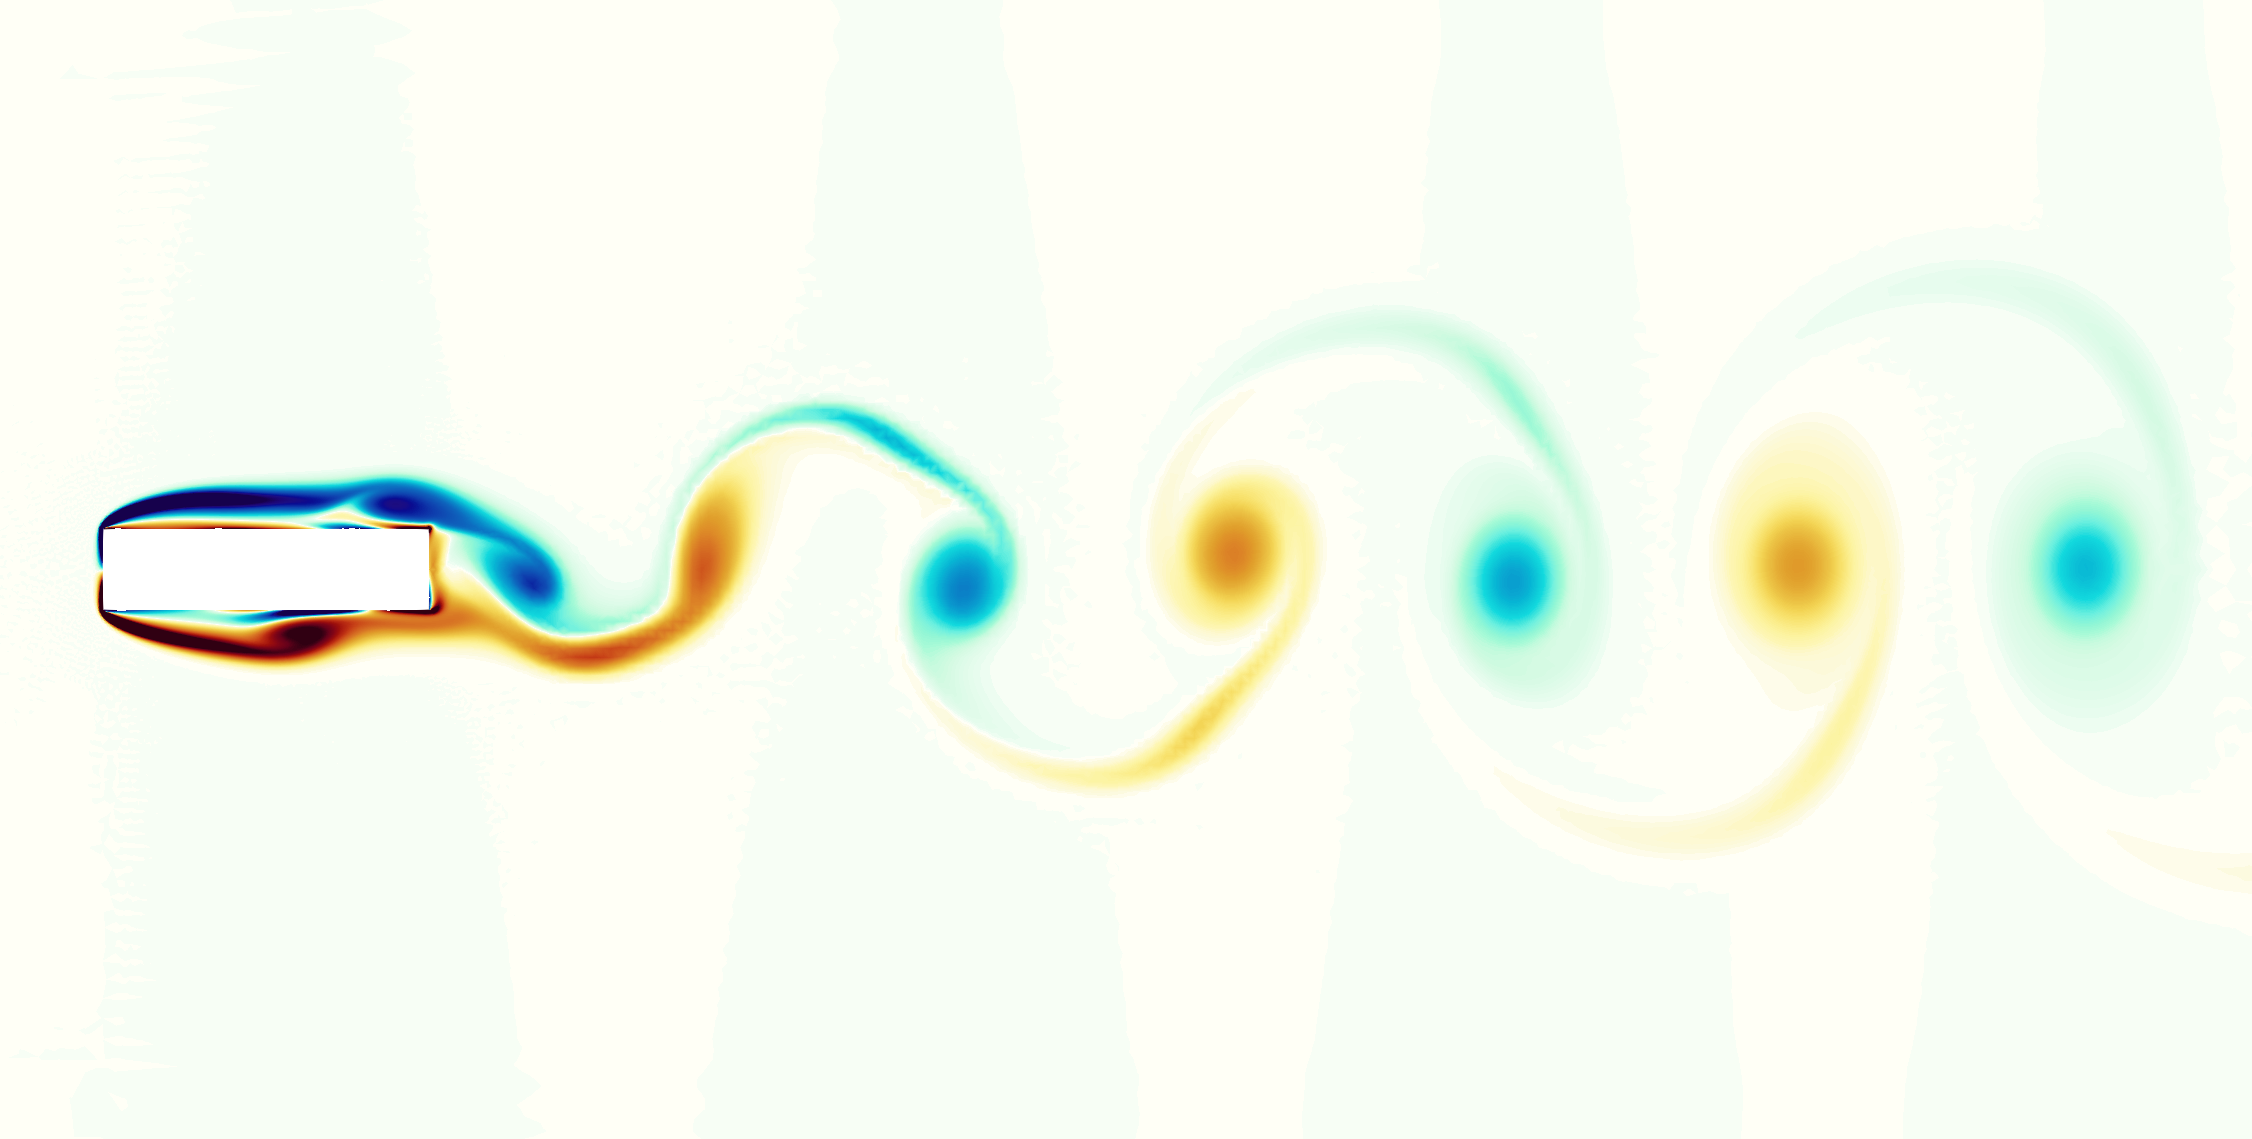
\includegraphics[trim={0 100 0 100},clip,width=0.49\textwidth]{./fig/vort_Re425_50.png}
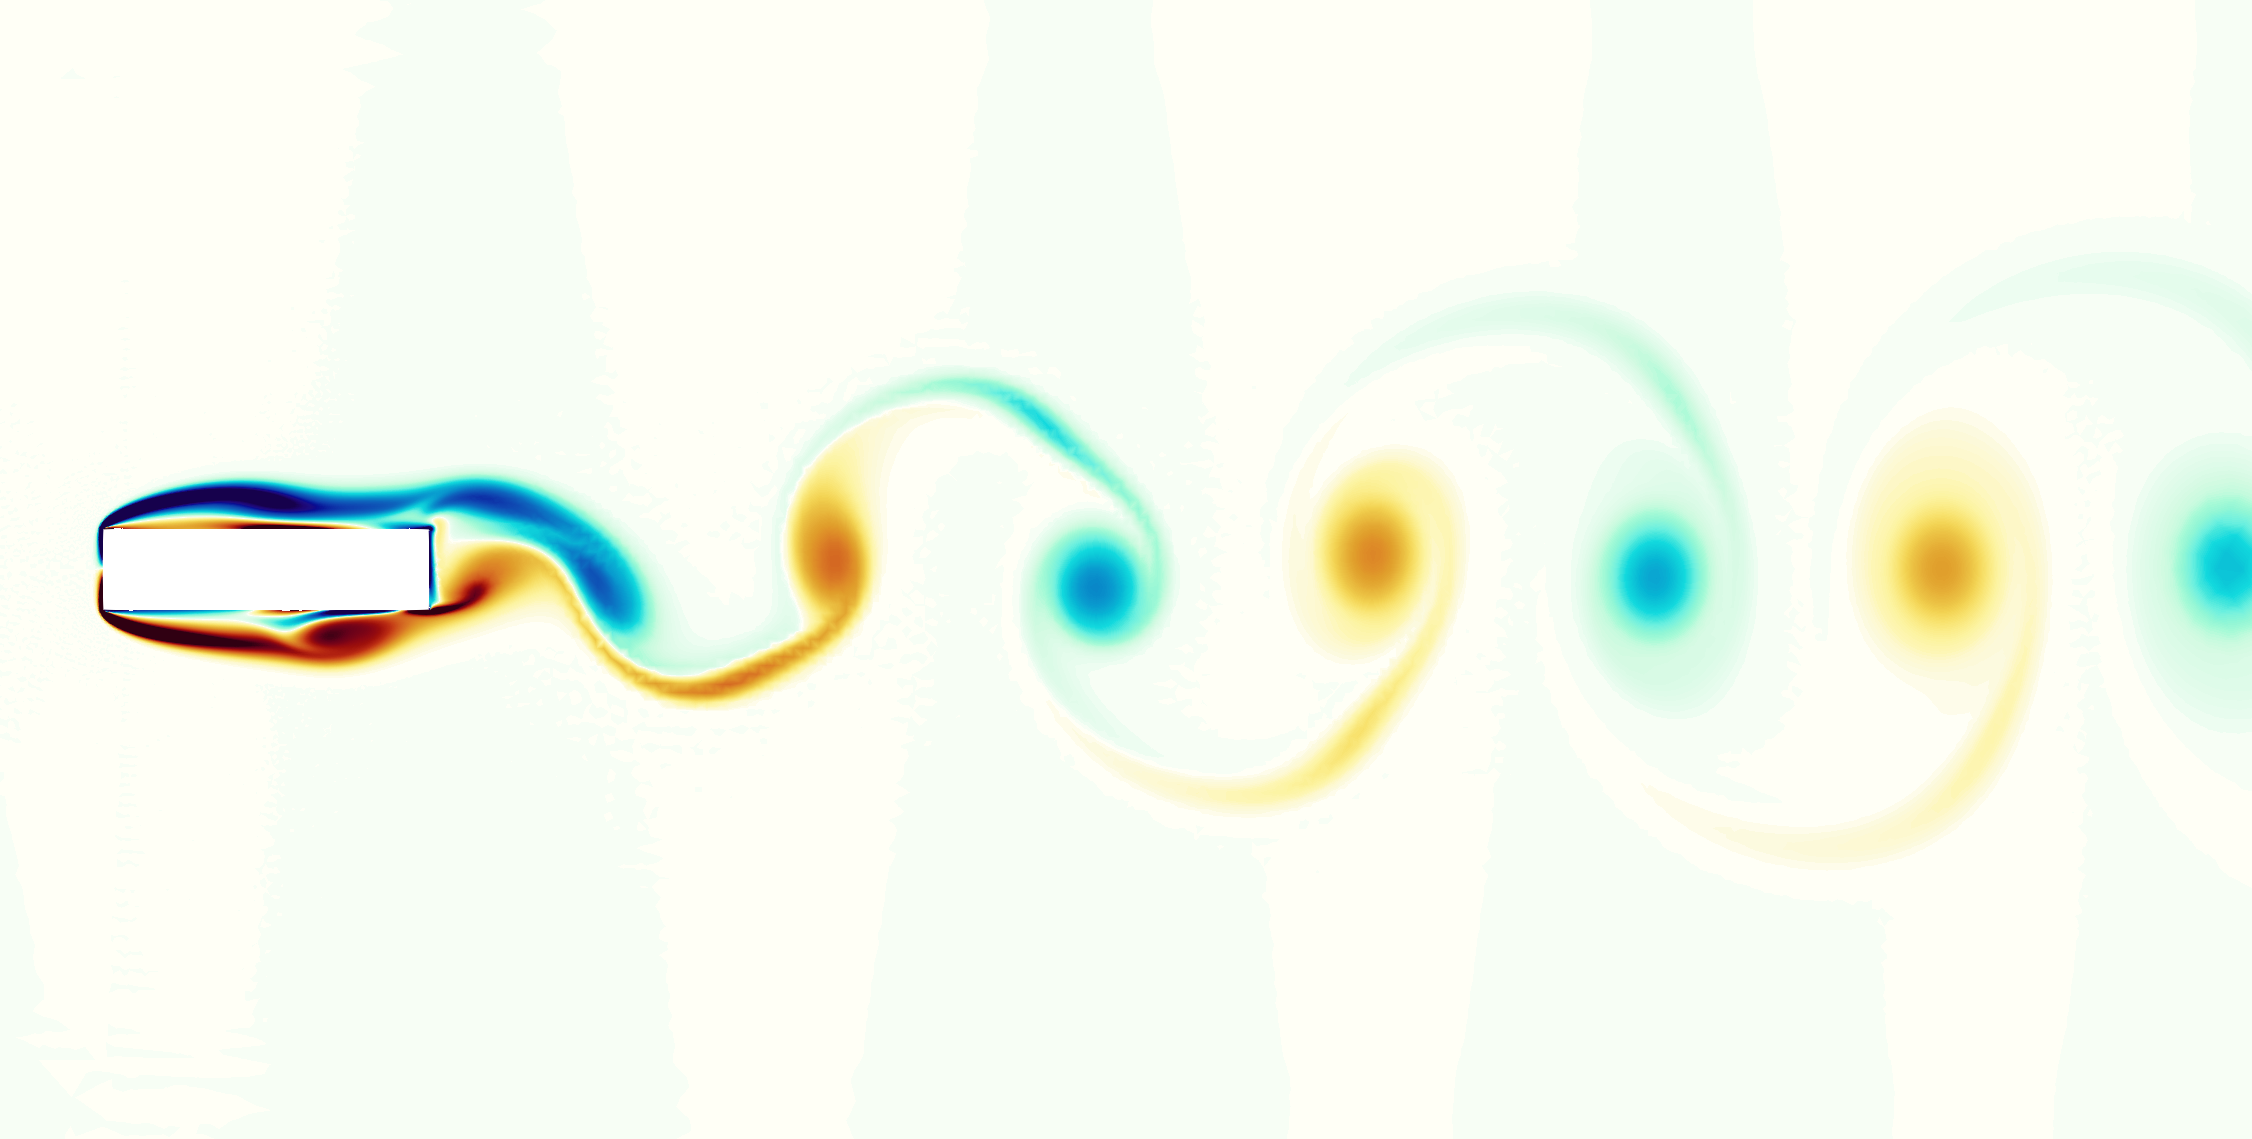
\includegraphics[trim={0 100 0 100},clip,width=0.49\textwidth]{./fig/vort_Re425_75.png}
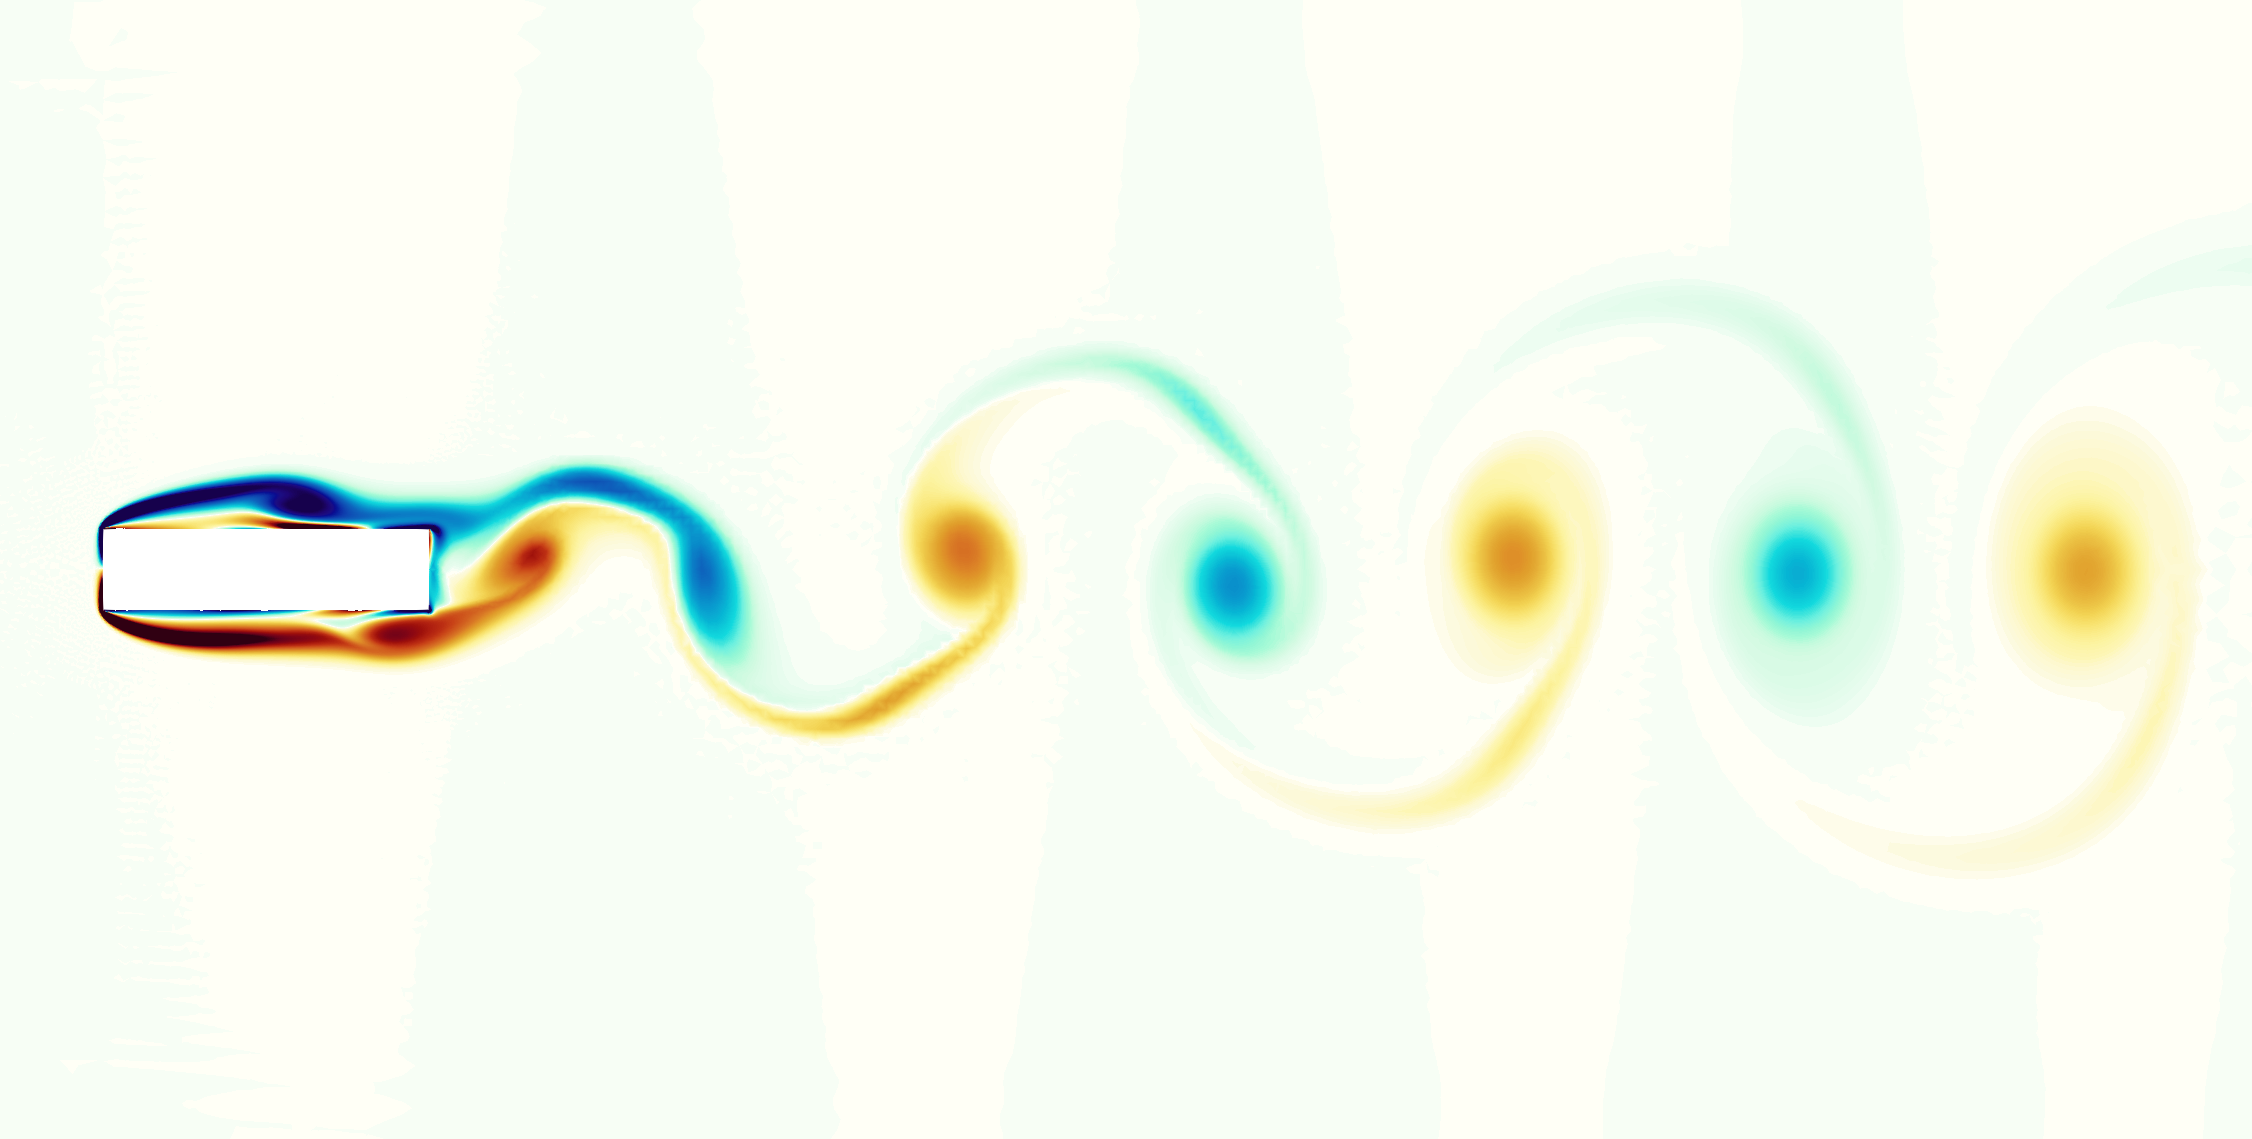
\includegraphics[trim={0 100 0 100},clip,width=0.49\textwidth]{./fig/vort_Re425_100.png}
\vspace{0.1cm}
\begin{tikzpicture}
\draw (-10,2) -- (8,2);
\end{tikzpicture}
\vspace{0.1cm}
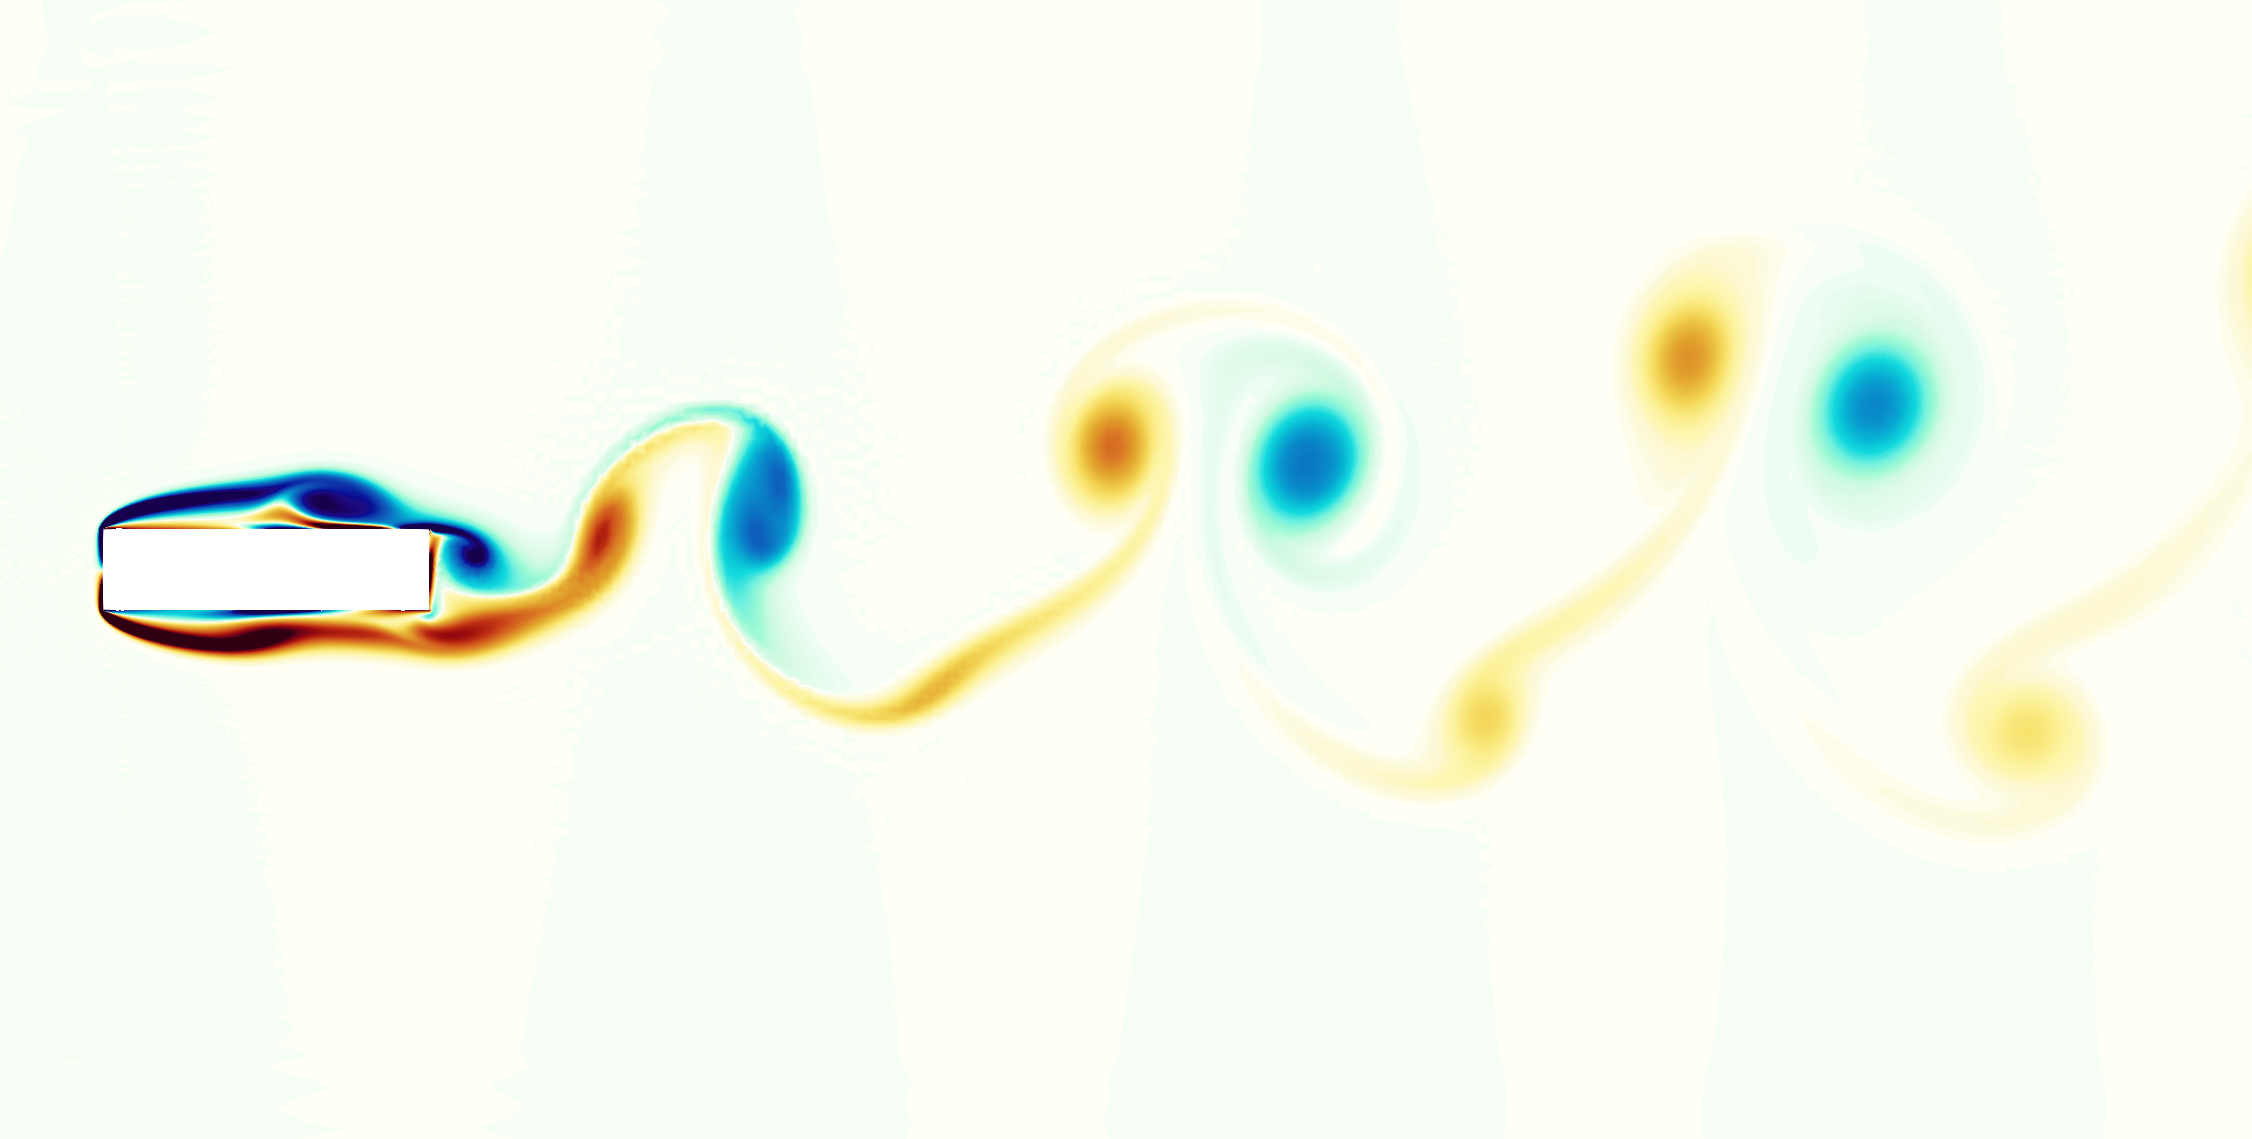
\includegraphics[trim={0 100 0 100},clip,width=0.49\textwidth]{./fig/vort_Re450_25.png}
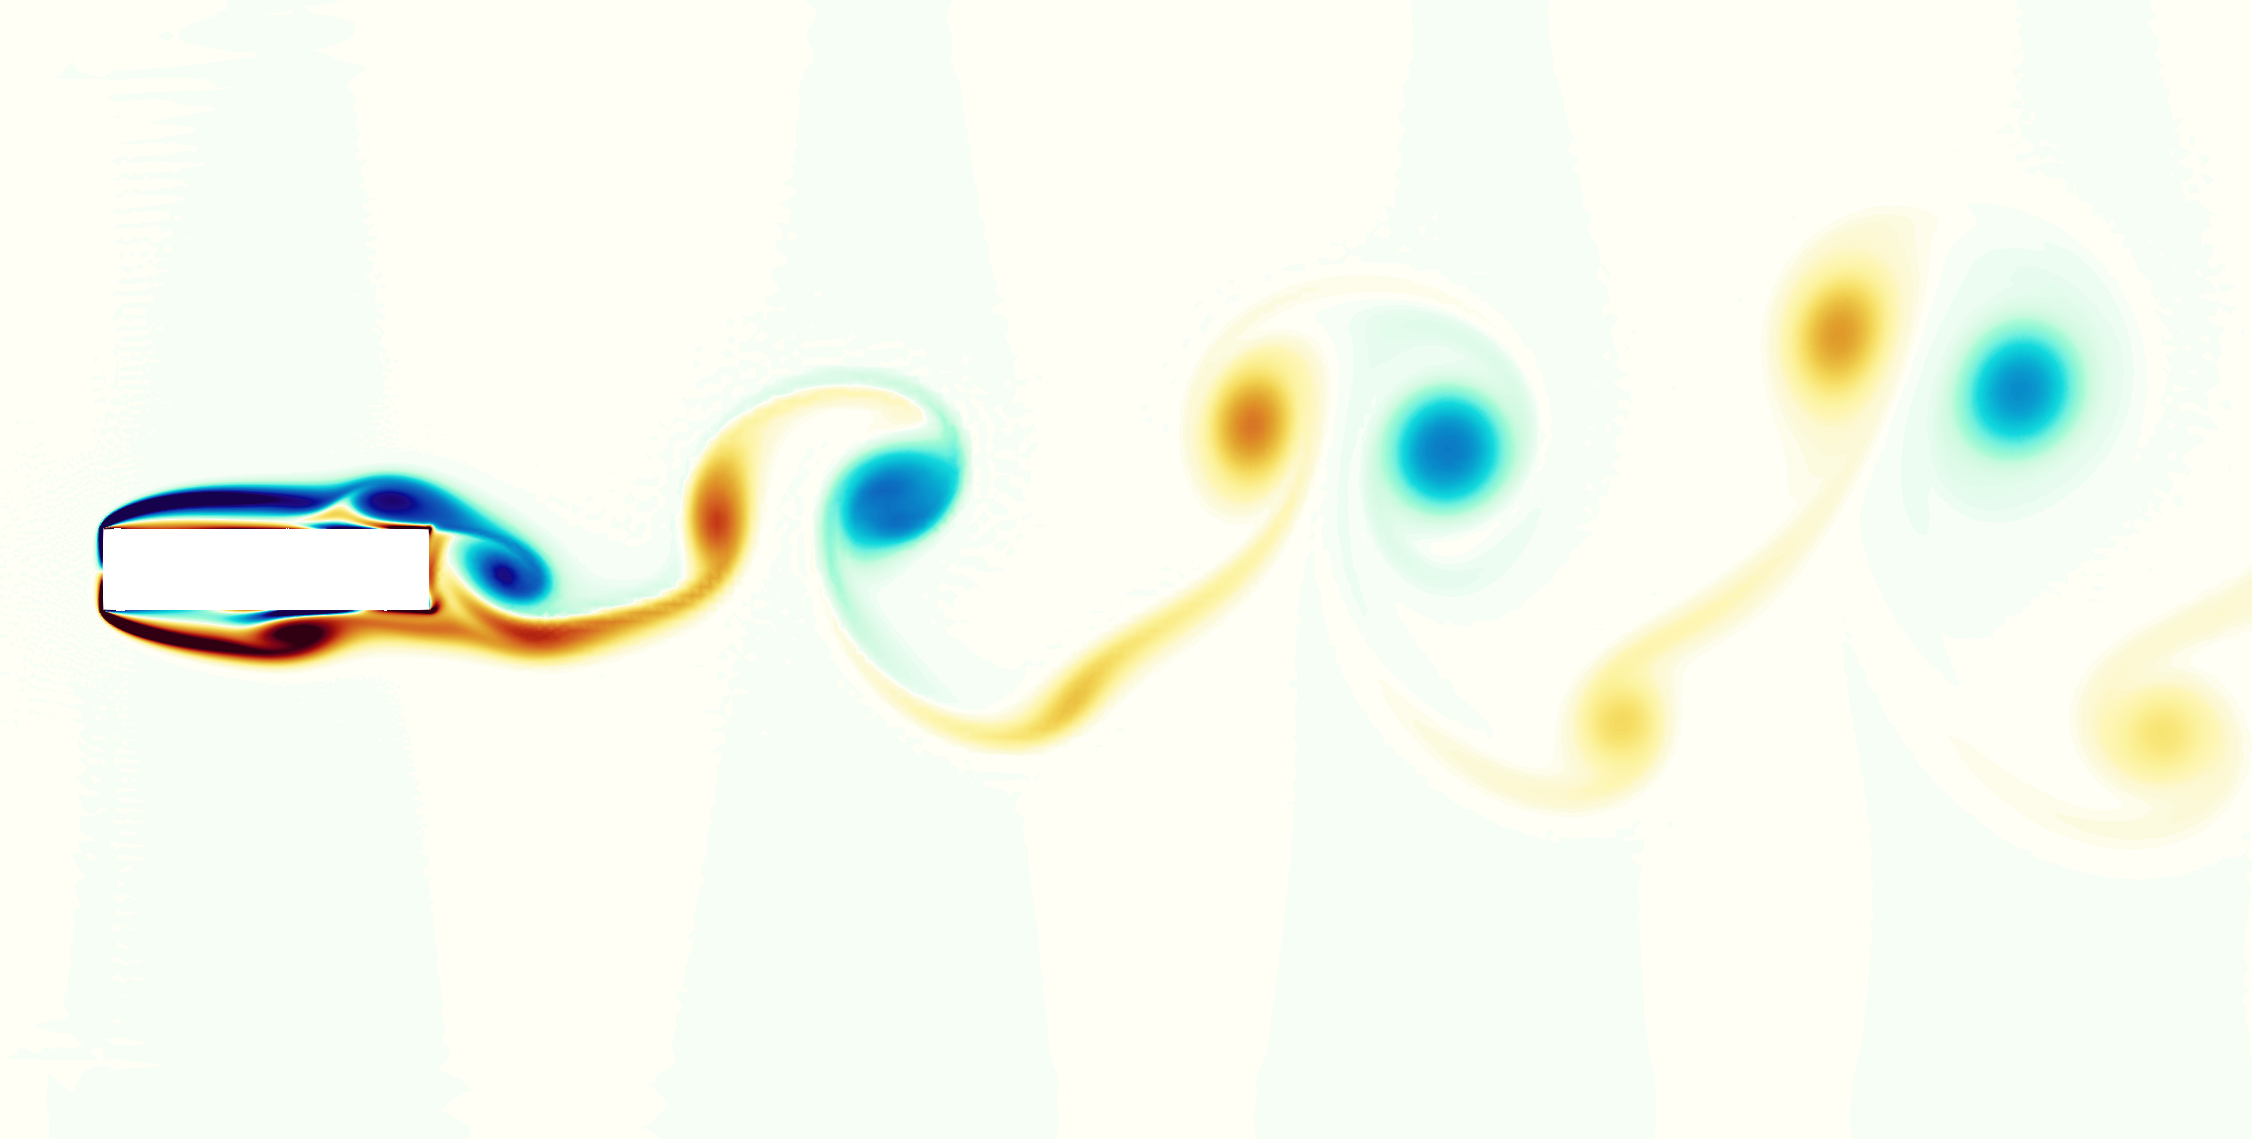
\includegraphics[trim={0 100 0 100},clip,width=0.49\textwidth]{./fig/vort_Re450_50.png}
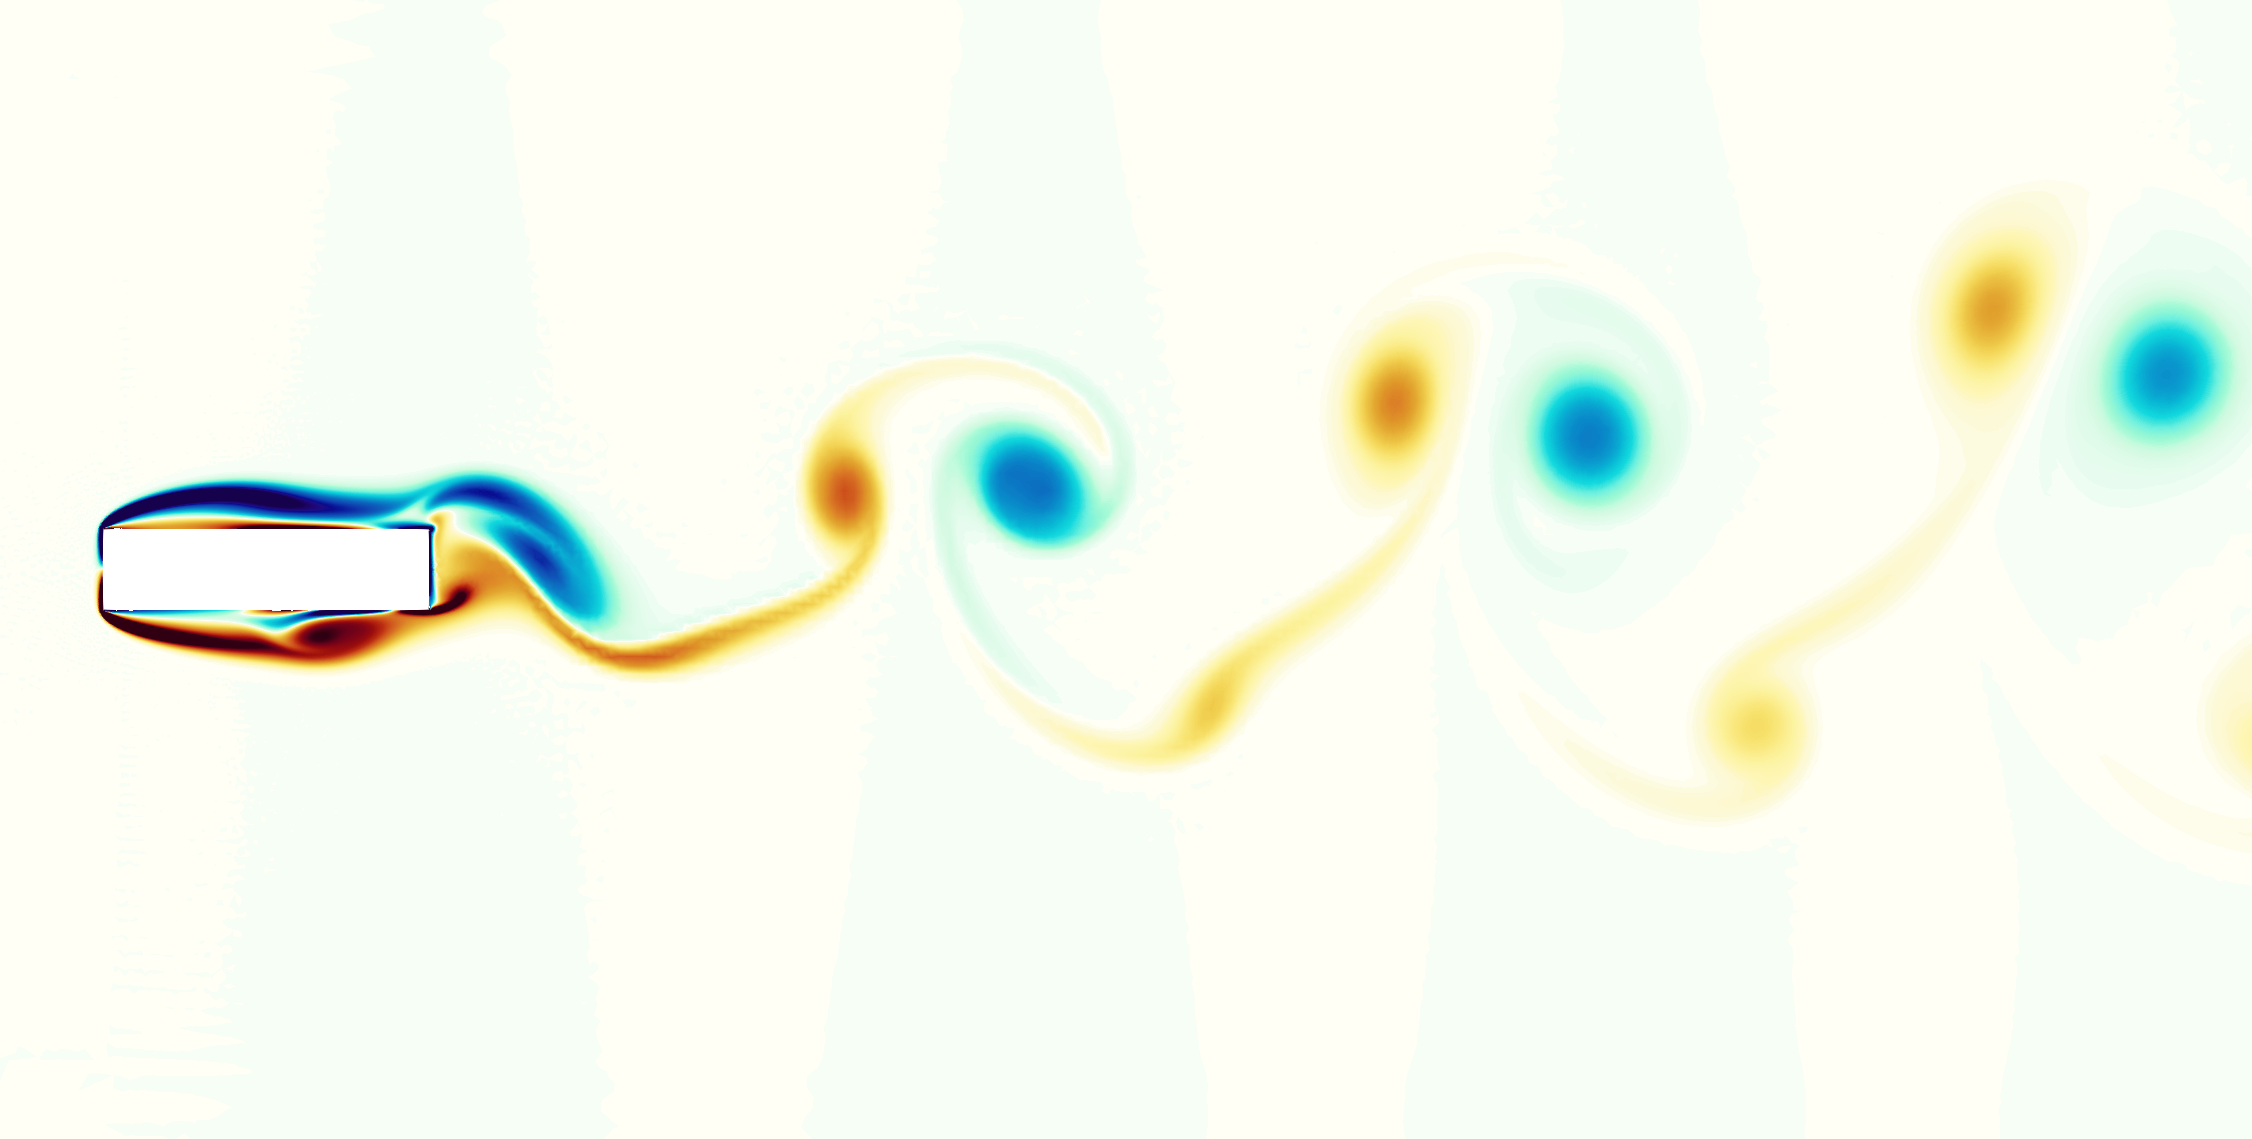
\includegraphics[trim={0 100 0 100},clip,width=0.49\textwidth]{./fig/vort_Re450_75.png}
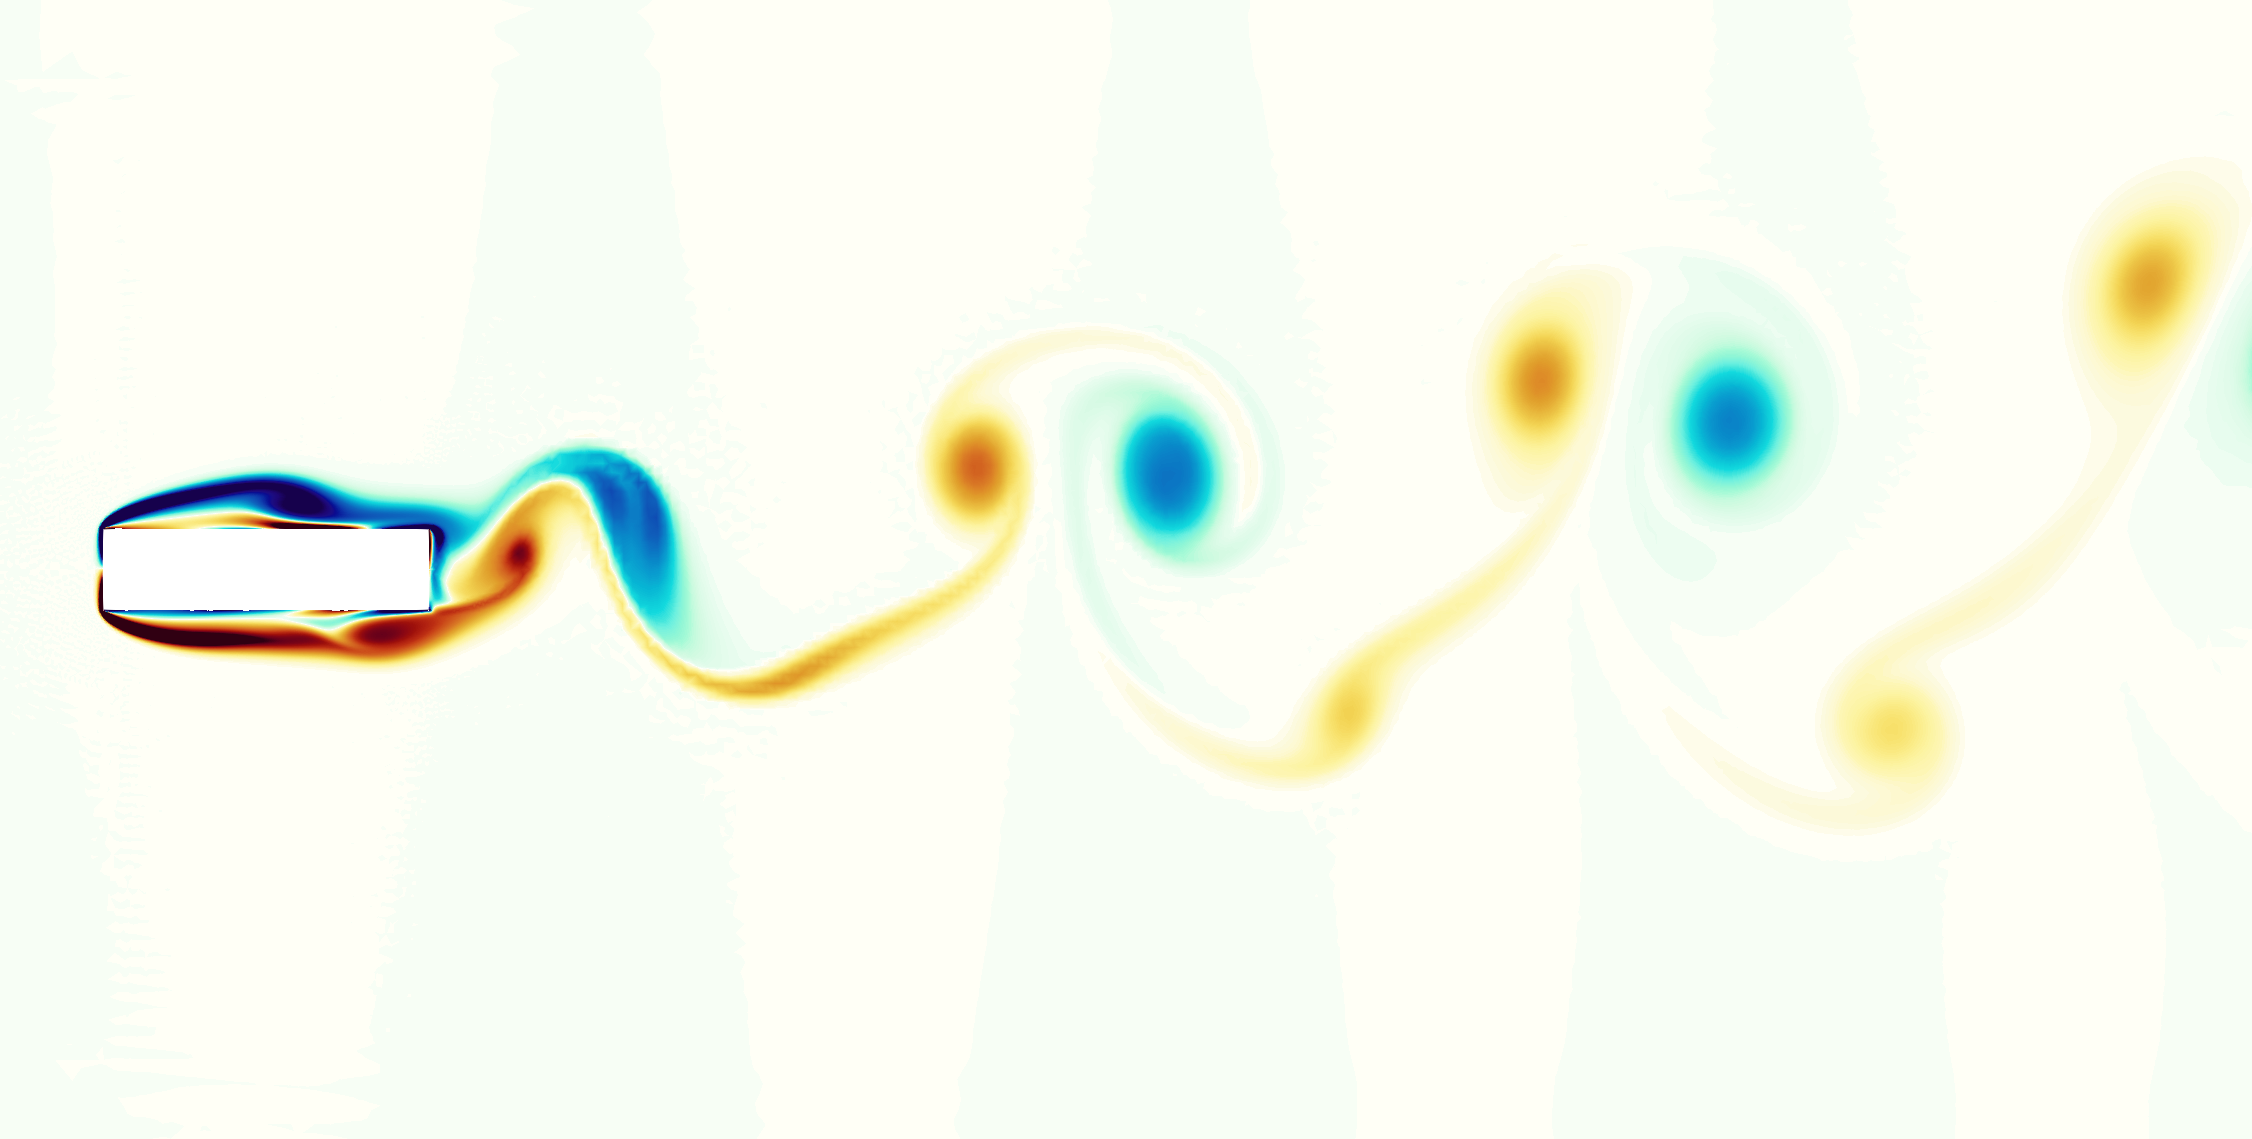
\includegraphics[trim={0 100 0 100},clip,width=0.49\textwidth]{./fig/vort_Re450_100.png}
\caption{Top: Evolution of the vorticity in one oscillation period for $\AR=4$ and $Re=425$. Bottom: Evolution of the vorticity in one oscillation period for $\AR=4$ and $Re=450$.}
\label{fig:vort_AR4_Re425}
\end{figure}

\begin{figure}
\centering
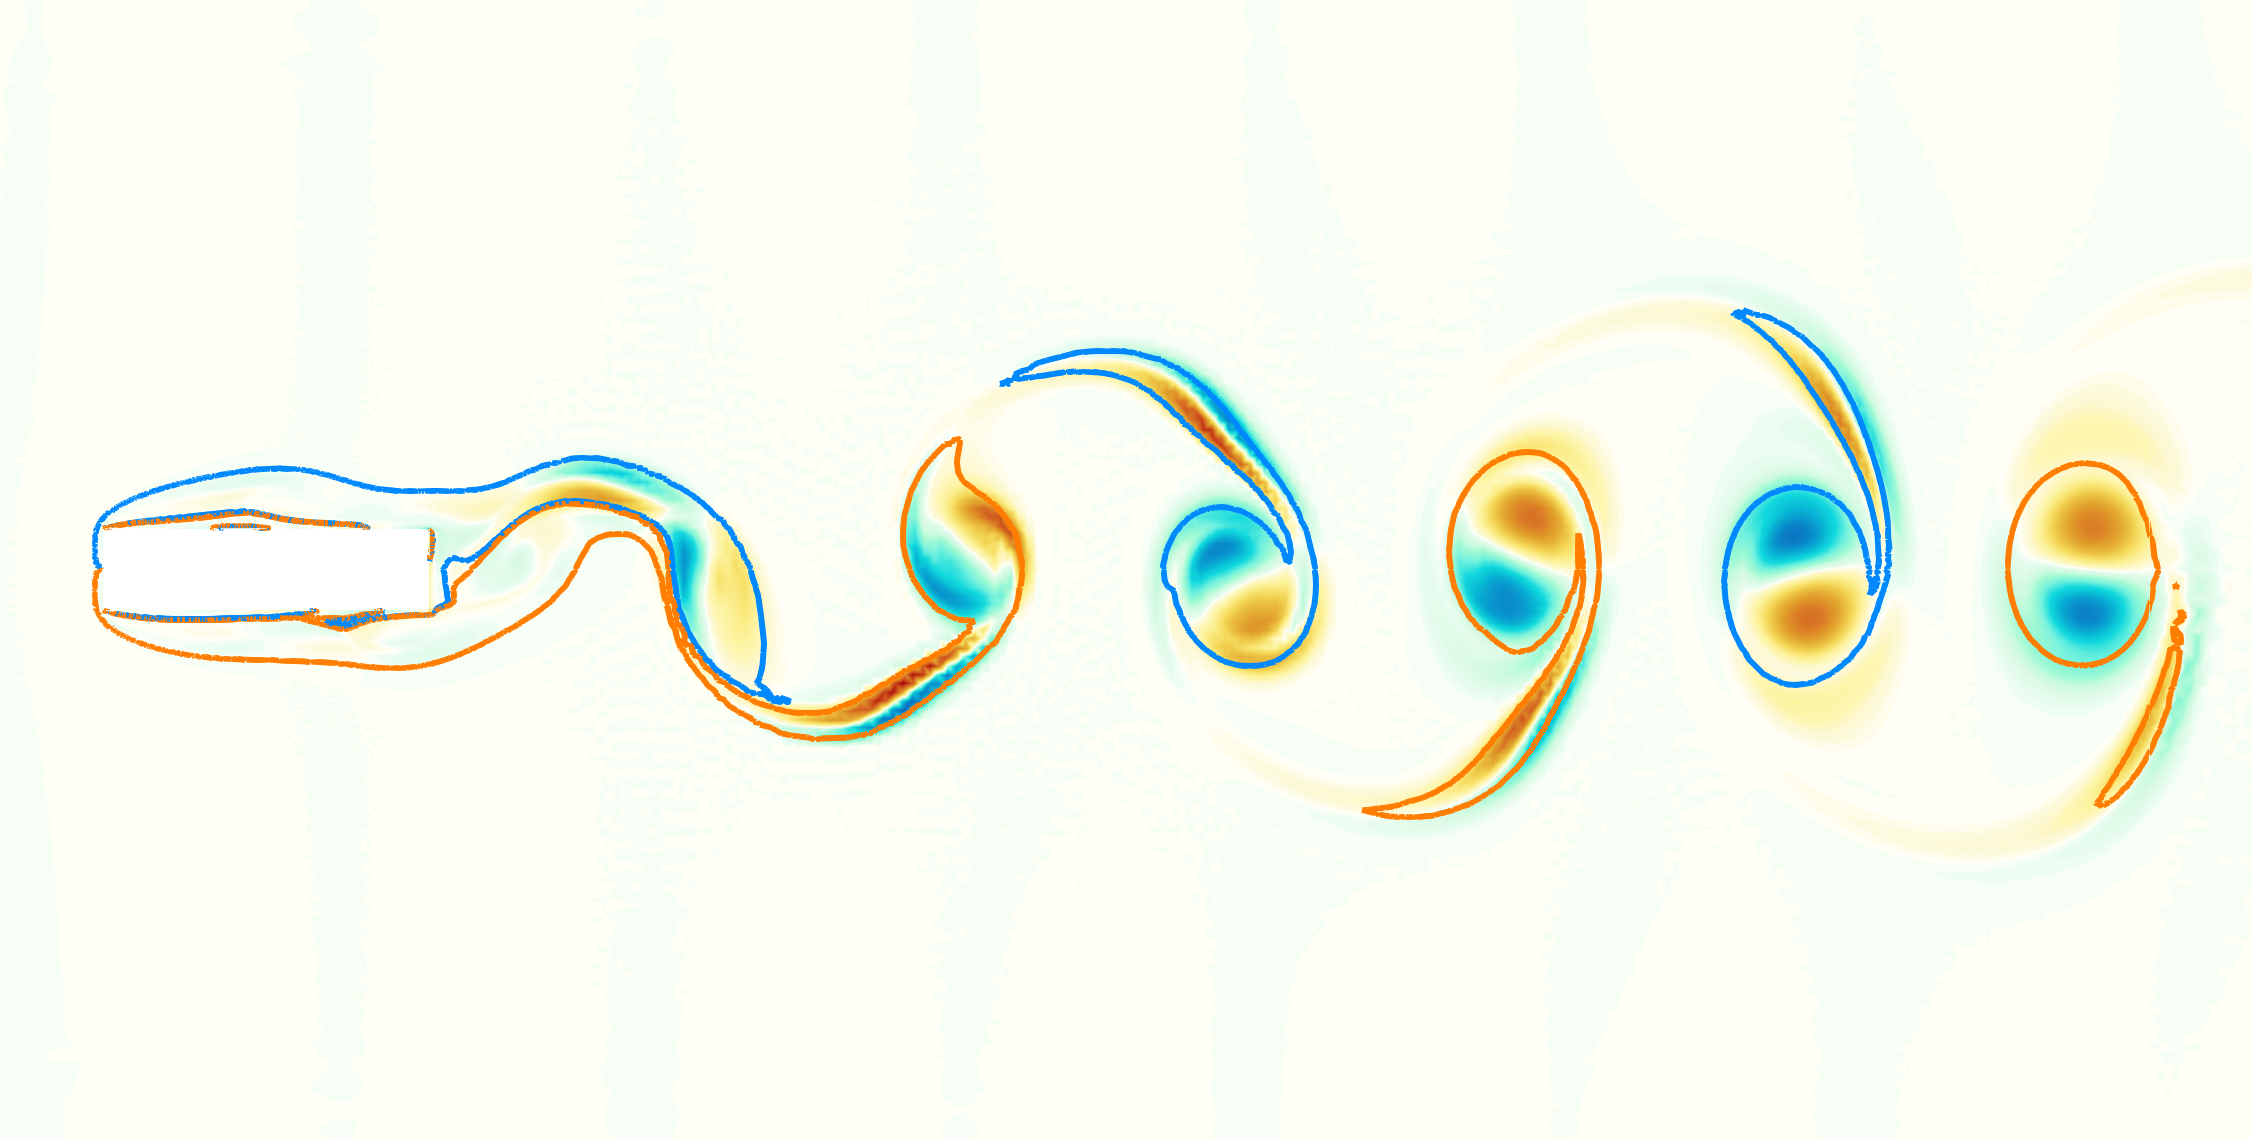
\includegraphics[trim={0 200 0 200},clip,width=0.7\textwidth]{./fig/omegaz_beta0_Re425.png}
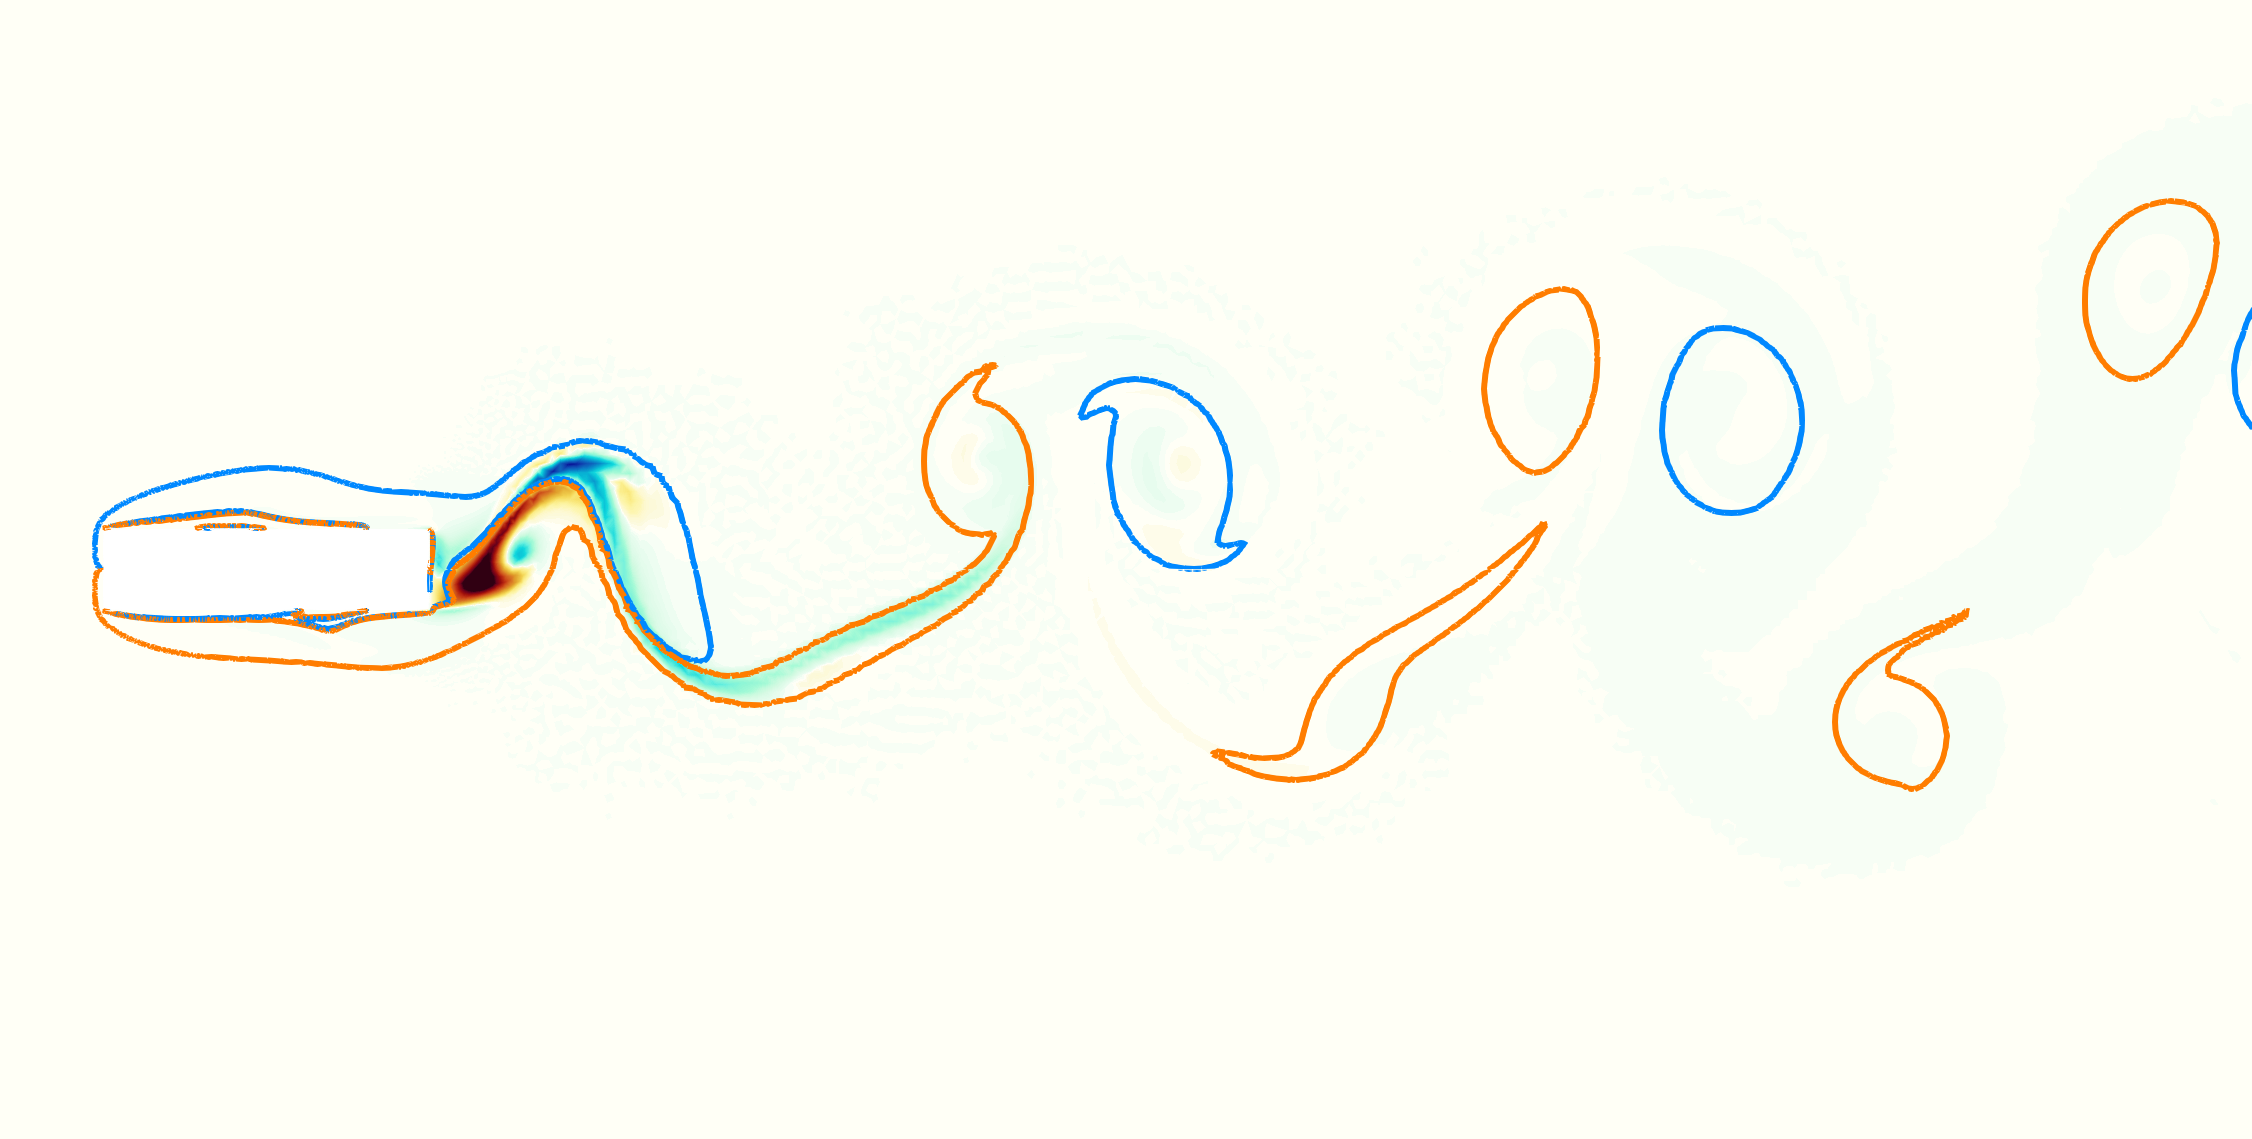
\includegraphics[trim={0 200 0 200},clip,width=0.7\textwidth]{./fig/omegaz_beta7p5_Re450.png}
\caption{Top: Floquet mode $\hat{\omega}_z$ for $\AR=4$, $Re=425$ and $\beta=0$. The isolines are vorticity of the base flow. Bottom: Floquet mode $\hat{\omega}_z$ for $\AR=4$, $Re=450$ and $\beta=7.5$. The isolines are vorticity of the base flow.}
\label{fig:AR4_Floquet_modes}
\end{figure}

\begin{figure}
\centering
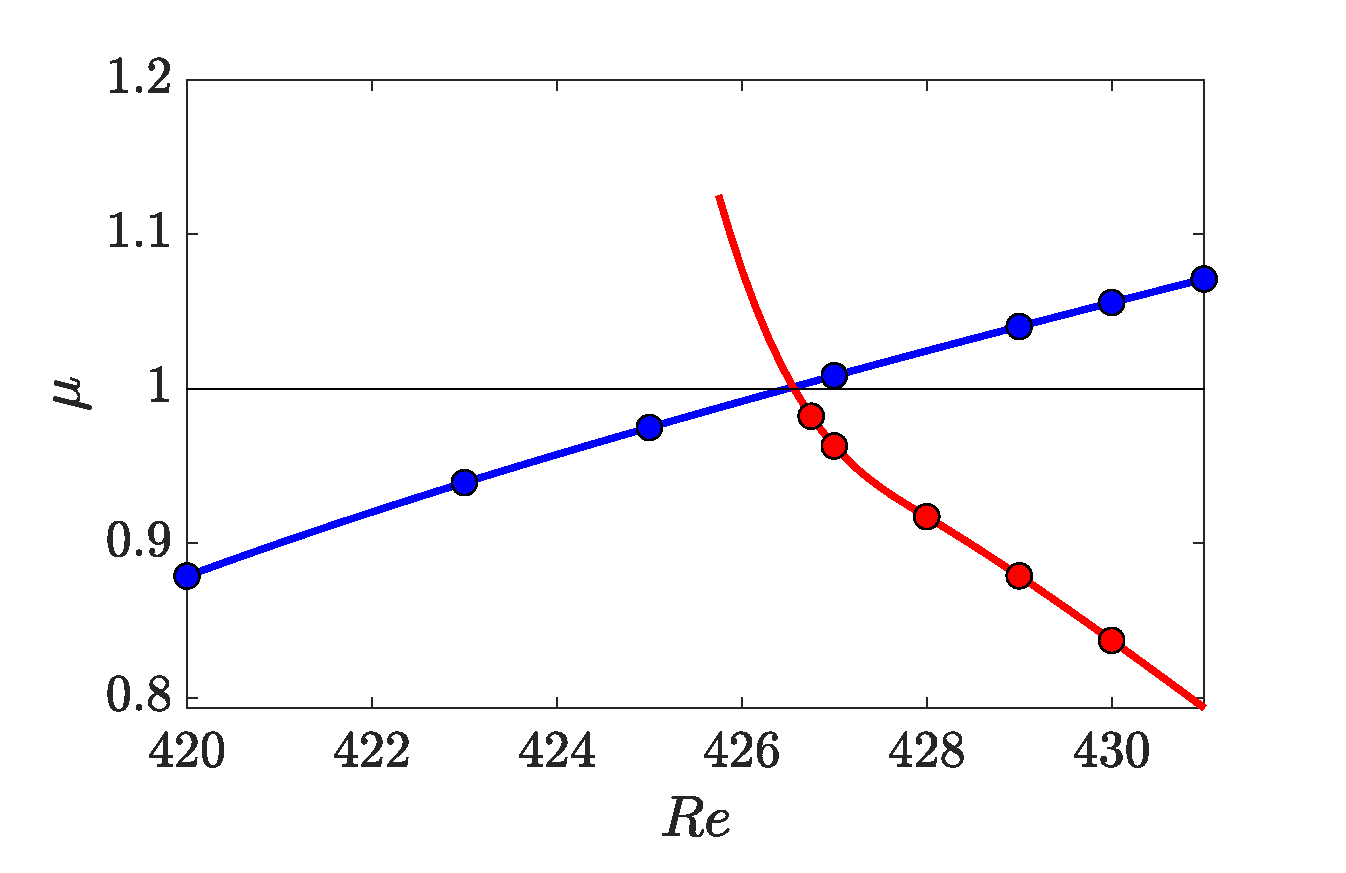
\includegraphics[width=0.49\textwidth]{./fig/AR4_2Dbif_multipliers.eps}
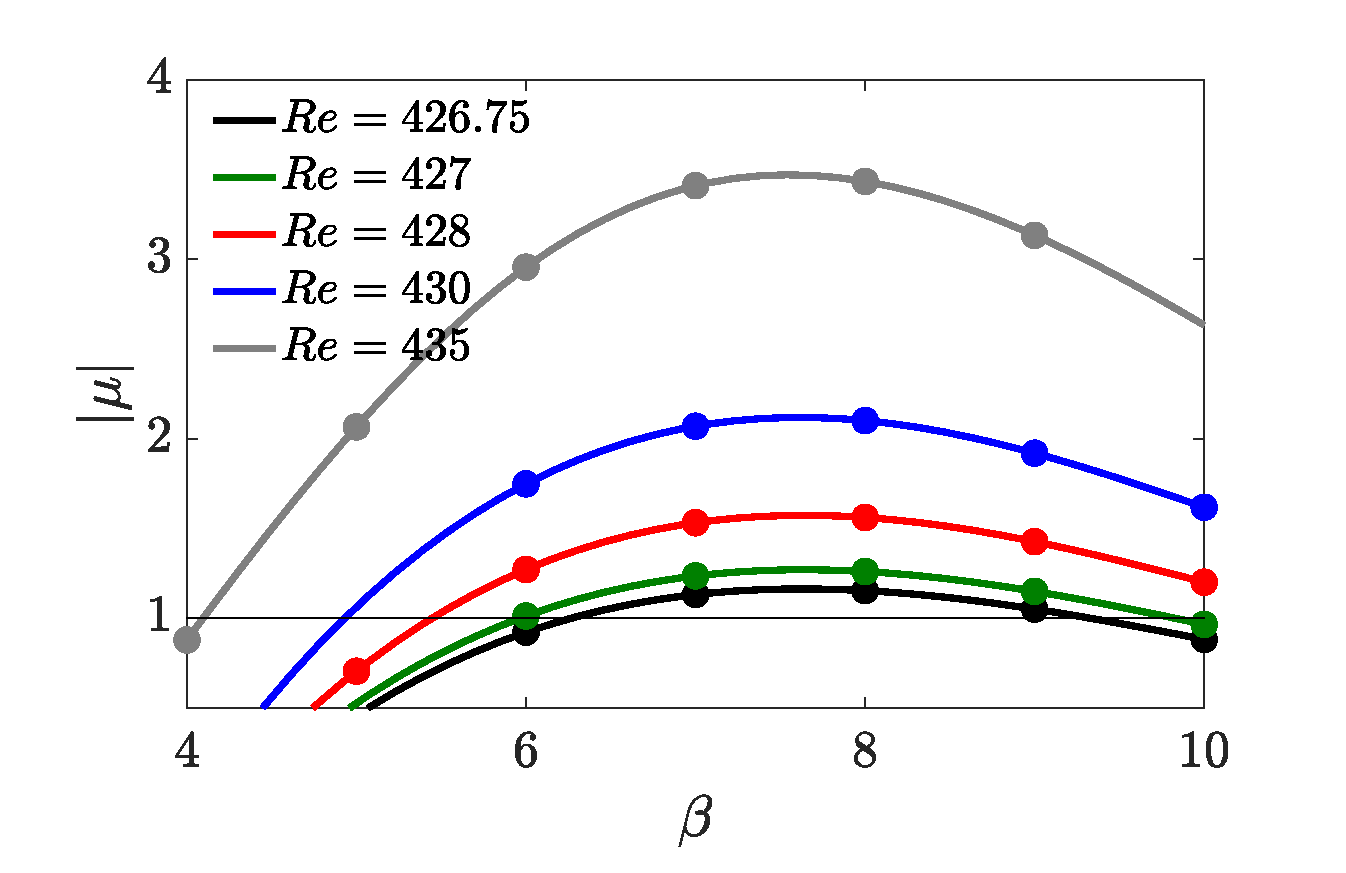
\includegraphics[width=0.49\textwidth]{./fig/AR4_3Dbif_multipliers.eps}
\caption{Left: Stability margin for the straight and slanted wake configuration. The blue circles are the Floquet multipliers related to the base flow with straight wake configuration. The red circles are the Floquet multipliers related to the base flow with the slanted wake configuration. Right: Stability of the slanted wake configuration to three-dimensional perturbations. Modulus of the Floquet unstable floquet multipliers. {\color{red} Need to check the dependence of the results on the size of the computational domain}.}
\label{fig:2Dmultipliers}
\end{figure}

We start considering $\AR=4$, which is in the first horizontal branch of the $St-\AR$ curve. We observe that the flow regime changes as $Re$ increases. For $Re \le 425$ the flow is periodic and the wake is straight. For larger $Re$, instead, the wake experiences an additional bifurcation and becomes slanted. For this $\AR$, the flow experiences a secondary two-dimensional bifurcation towards a limit cycle with the same frequency, before becoming three-dimensional. This is visualised in figures \ref{fig:vort_AR4_Re425} and \ref{fig:vort_AR4_Re450} where flow snapshots are shown for $Re=425$ and $Re=450$. For the lowest $Re$ the wake is straight and characterised by the usual alternating shedding of vortices with positive/negative vorticity from the bottom/top sides of the cylinder. Note that vortices are shed also from the LE, and in agreement with previous results in literature, a single vortex is place at each time over the lateral sides. At $Re=450$, instead, we find a slanted wake. In this case, indeed, the vortex monopoles are not placed along the $y=0$ line, but progressively deviate a part. This has been observed for $Re \ge 435$. 

To investigate the origin of this phenomenon, we have studied the linear stability of the straight wake to two-dimensional perturbations, using Floquet theory; see figure \ref{fig:2Dmultipliers}. For $Re=425$ we have found a multiplier that is very lose to the unit circle being $\mu \approx (0.97,0)$. This agrees with the fact that at this $Re$ the straight wake is stable and that it becomes unstable at slightly larger $Re$. Also, the fact that $\Im(\mu)= 0$ confirms the fact that the slanted wake is the result of a synchronous global instability of the wake. To provide further details, in the top panel of figure \ref{fig:AR4_Floquet_modes} we show the structure of the Floquet mode with isolines of the base-flow vorticity. In the wake the unstable mode generates dipoles of spanwise vorticity that grow in space and time as they are advected downstream. A synchronisation between the base flow and the perturbation field is observed, with the dipoles of the linear mode being centred with the the base-flow vortices at all times. %
A dipolar perturbation of a monopolar vortex is often referred to as displacement mode \citep{brion-sipp-jacquin-2014} and is known to result in a displacement of the vorticity centroid, similarly to what observed in figure \ref{fig:vort_AR4_Re450}. We consider the first positive base-flow vorticity monopole in the wake. Here the Floquet dipole has positive vorticity in the upper part, and negative vorticity in the lower part. This superposition strengthens the top part of the monopole and weakens the bottom part, resulting into a net displacement of the monopole in the upward direction. In contrast, in the second monopole of negative base-flow vorticity the scenario is the opposite. The Floquet dipole has positive vorticity in the bottom part of the monopole, and negative vorticity in the top part %. This strengthens the top part of the monopole and weaken the bottom part, and result
resulting again into a upward shift of the monopole. This explains the vertical displacement of the vortex centroids shown in figure \ref{fig:vort_AR4_Re450}. Overall, this mechanism resembles what observed in \cite{jallas-marquet-fabre-2017} in the case of pitching airfoils.


%
Notably, this new slanted wake is strongly unstable to three-dimensional perturbations of subharmonic nature, being characterised by a small spanwise wavelenght (a large value of $\beta$); see figure \ref{fig:2Dmultipliers}. The linear stability of the slanted wake to three-dimensional perturbations has been investigated again by mean of Floquet analysis. For $Re \ge 435$ we have found a Floquet multiplier outside the unit circle, having negative imaginary part. For $Re=450$ we found $ mu \approx (-4.8,0)$ for $\beta=7$ ({\color{red} we still have to study the dependence of the results on the vertical extent of the computational domain}). The 
structure of the mode is shown in the bottom panel of figure \ref{fig:AR4_Floquet_modes}. This is clearly an unstable mode of the wake. The mode, indeed, in almost null over the lateral sides of the cylinder where instead the flow dynamics is driven by the vortices shed by the LE.




\begin{itemize}
  \item It is still not clear whether the slanted wake is stable for a certain range of $Re$. It actually seems that when the wake becomes slanted it is immediately unstable to three-dimensional perturbations. How is it possible?
  \item After characterising the linear stability of the straight- and slanted-wake configuration it would be interesting to investigate the influence of the non linearity. We can follow the same approach proposed by \cite{jallas-marquet-fabre-2017}. We can stabilise the bifurcation, and write the non linear perturbation at a certain $Re$ as $\{ \bm{u}'',p'' \} = \{\bm{u},p \} - \{\bm{u}_S,p_S \}$, where we use the $\cdot_S$ subscript when referring to the symmetric configuration. At this point we have can plot the perturbation and discuss it. Also, we may also divide it is the symmetric and anisymmetric part to then address what is the influence of the two symmetric and asymmetric modes. Before doing this, we need to use BoostConv to symmetrise the flow, and compute the forces, to understand which is the question we want to address.
  \item Is the mechanism associated with the instability a viscous one? A possible approach would be to perform the Floquet stability by progressively increasing the $Re$?
  \item Also, why the flow becomes suddenly unstable to 3D perturbations once the wake becomes slanted? That mode is not present in the spectrum of the straight wake. My idea is that the feedback that leads to this mode is associated with something close to the trailing edge that appears only in this case. What about looking again at the close orbits, like Giannetti (2010)? We have already tried in a different set up, and we already have the code for this kind of computations.
  \item The scenario seems to hold also for $\AR=4.5$; see figure \ref{fig:vort_AR4p5_Re450}. Actually, in this case flow the low-$Re$ straight wake we observe two multipliers that approach the unit circle for $\beta=0$. One is real and positive (as for $\AR=4$), while one is complex. However, the structure of the mode is similar in both cases (see figure \ref{fig:AR4p5_modes_Re430_beta0}. For $Re=430$ they are $\mu = (1.249,0)$ and $\mu=(0.7949, \pm 0.52)$. Also, once the wake settles to the slanted configuration, similarly to what observed for $\AR=4$ we observe that it is strongly unstable to 3D perturbations with a small spanwise wavelength. Overall, this has been confirmed by Direct numerical simulations; see figure \ref{fig:lambda2_omegax_AR45_Re450}.
\end{itemize}

\begin{figure}
\centering
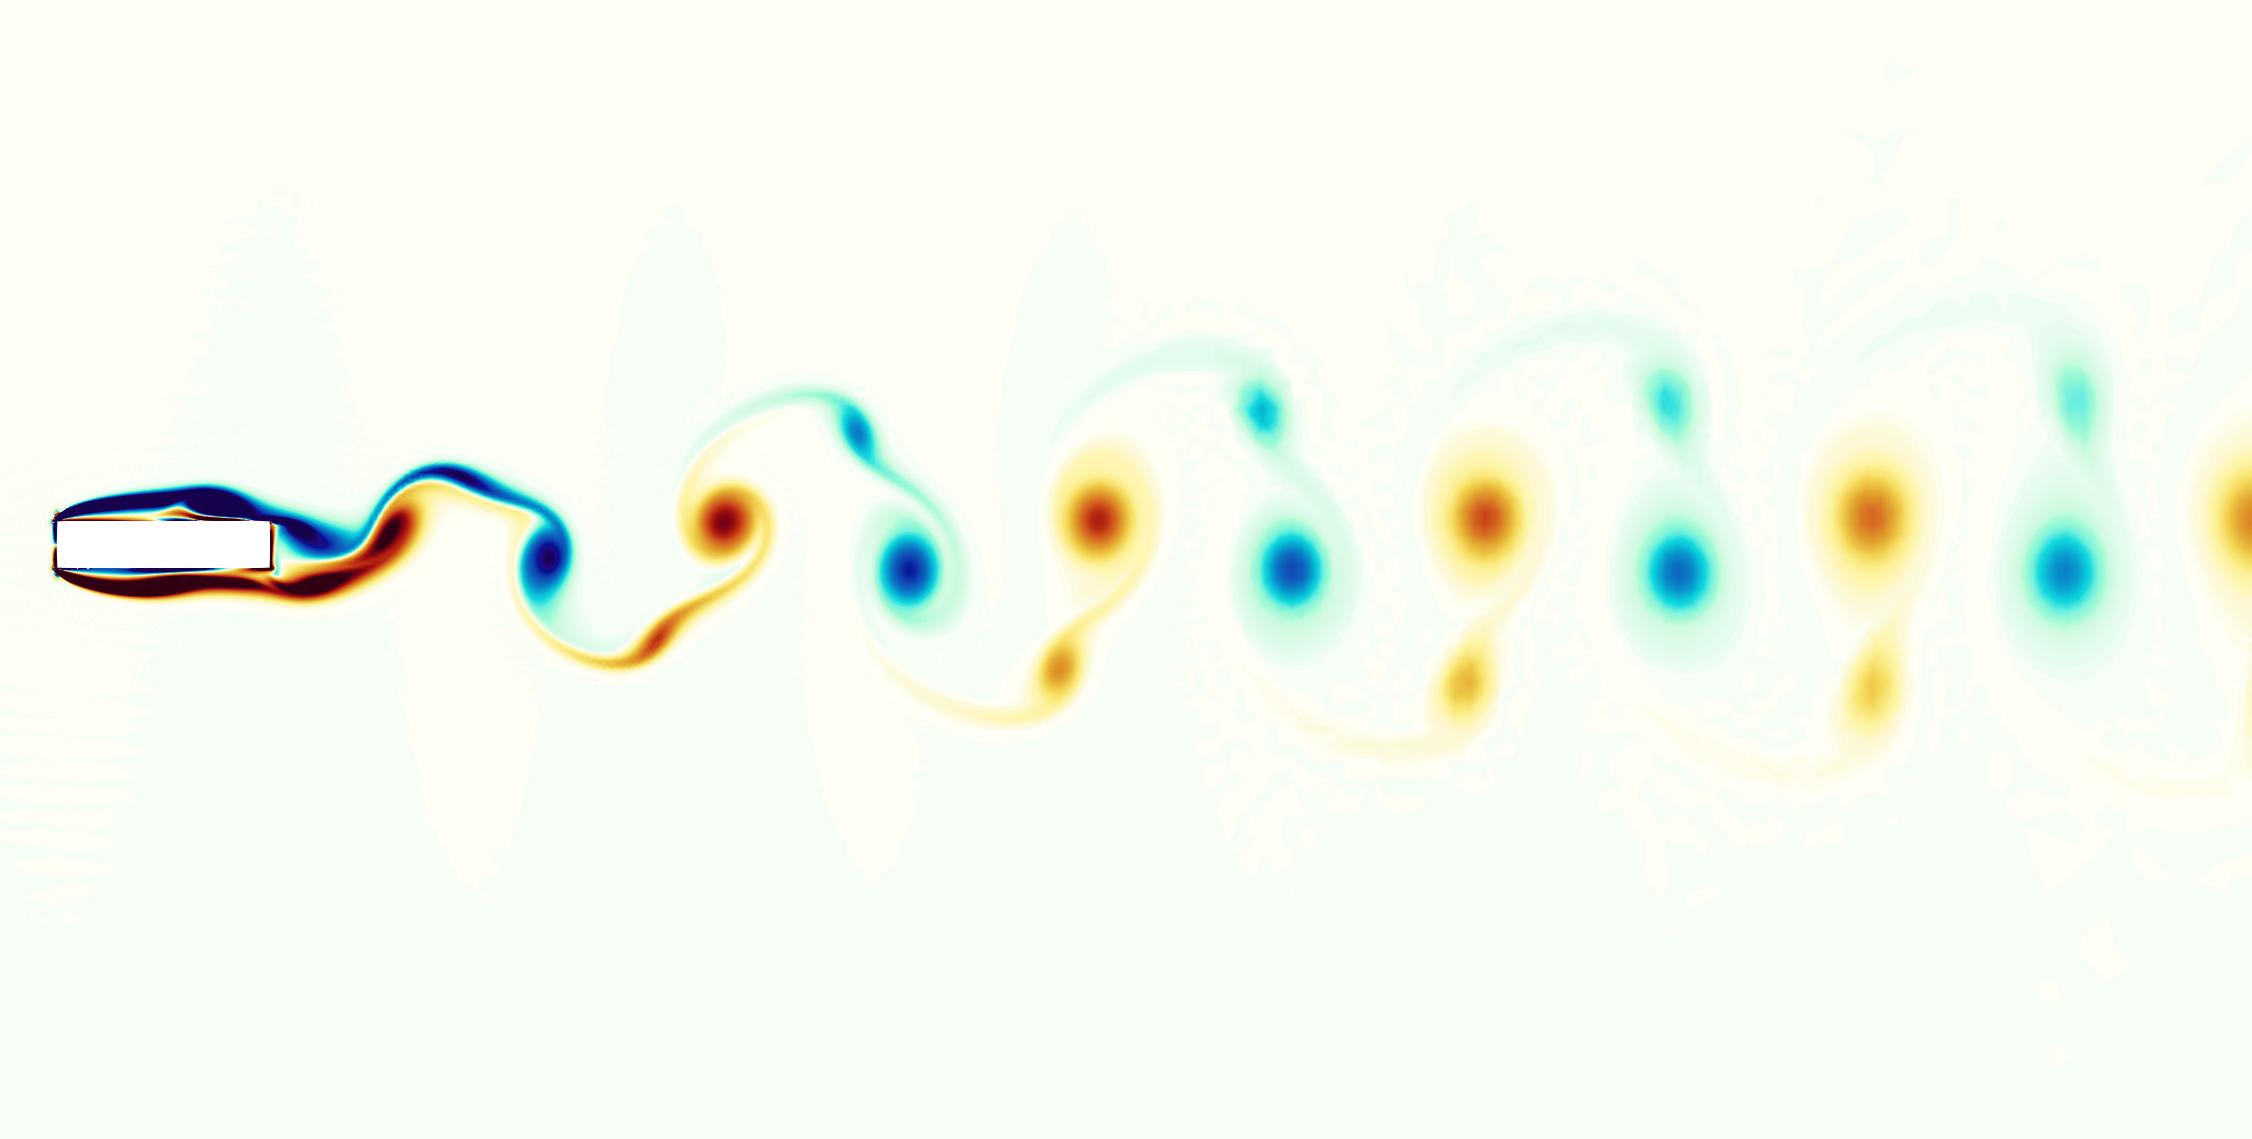
\includegraphics[trim={0 100 0 100},clip,width=0.49\textwidth]{./fig/AR4p5/vort_Re430_25.png}
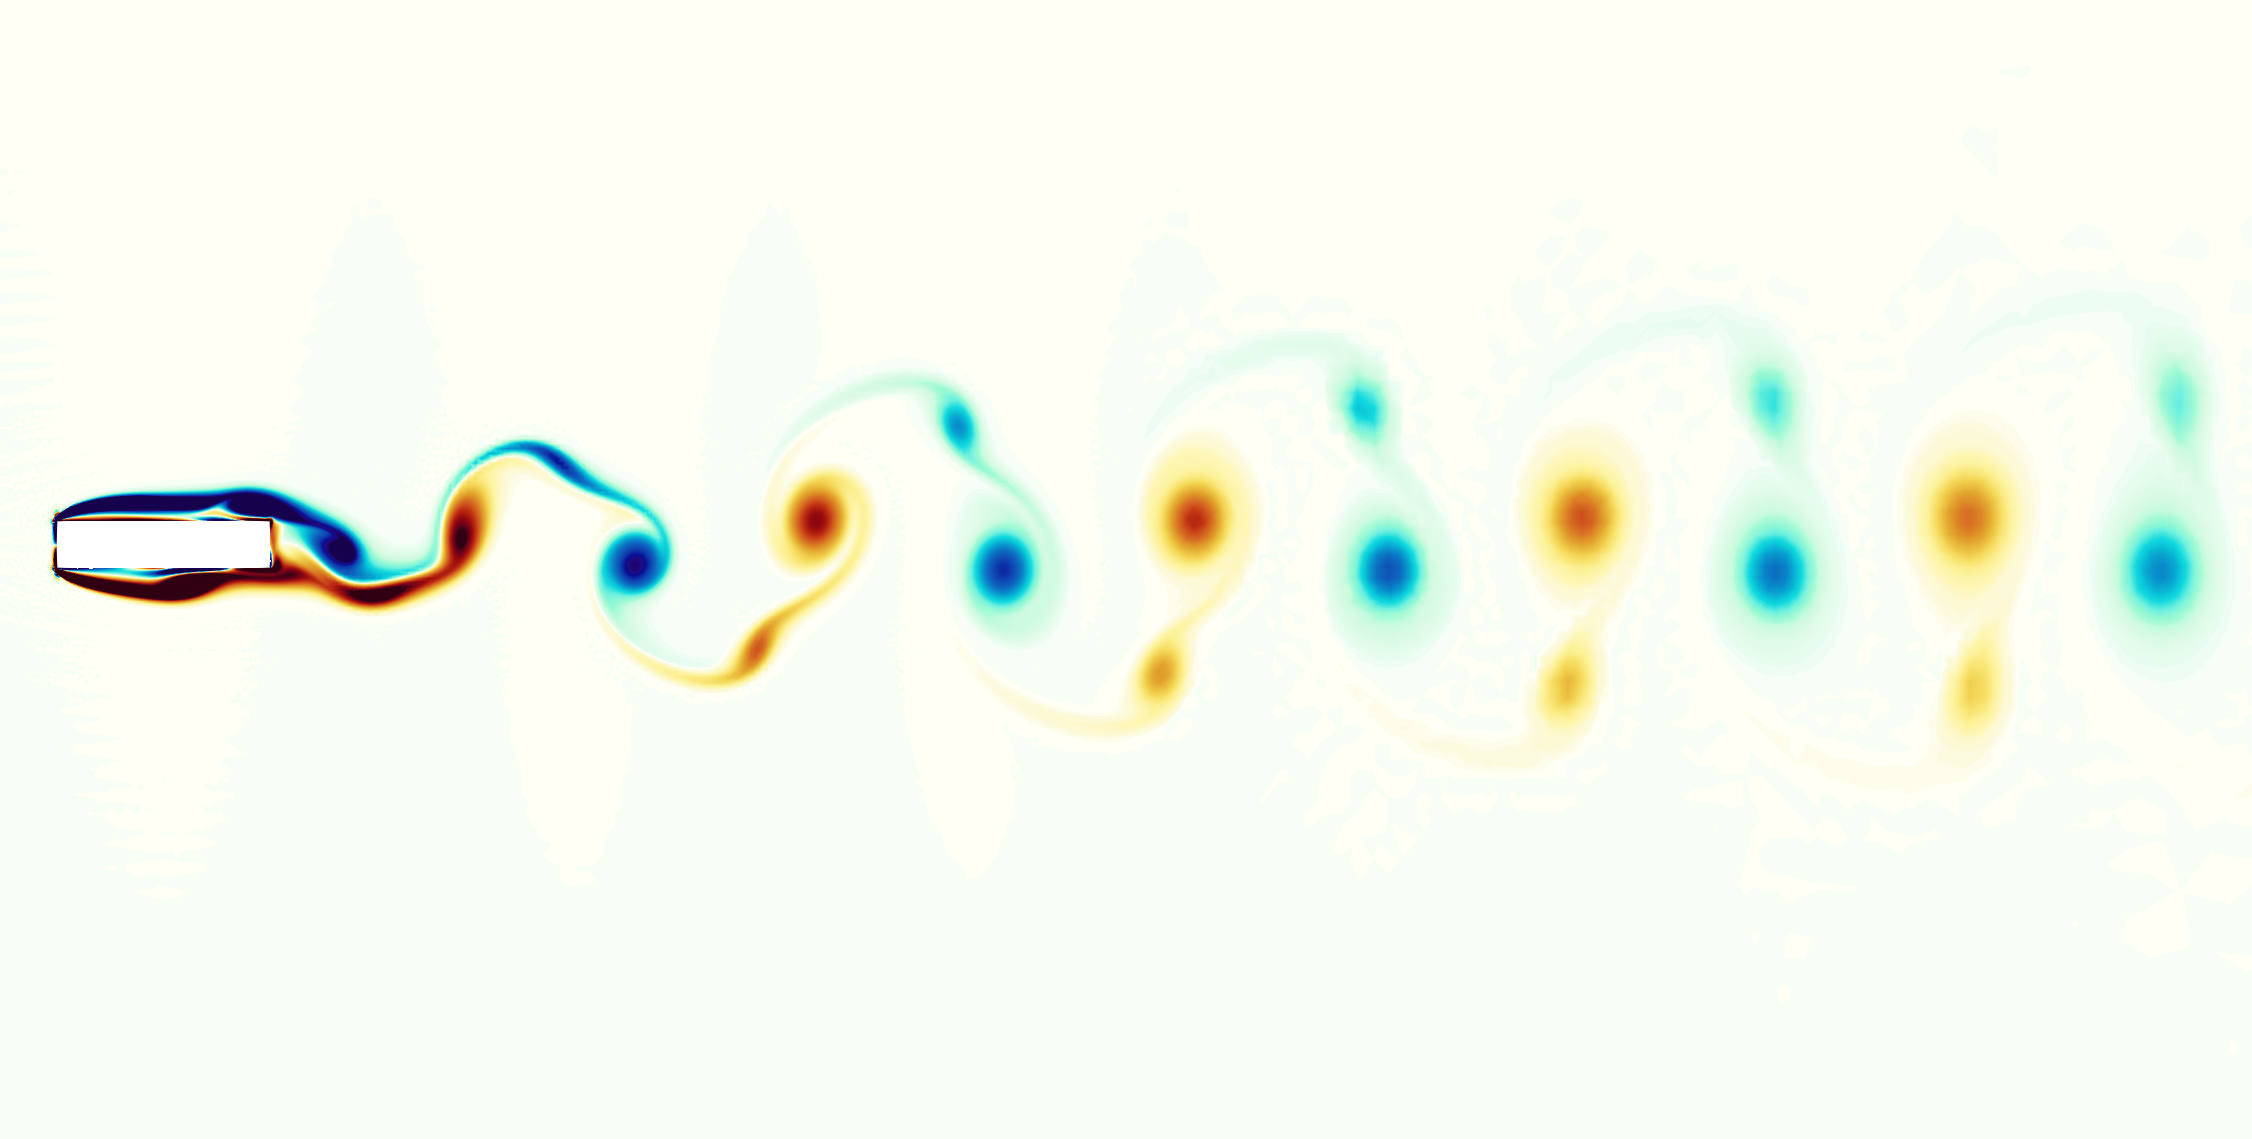
\includegraphics[trim={0 100 0 100},clip,width=0.49\textwidth]{./fig/AR4p5/vort_Re430_50.png}
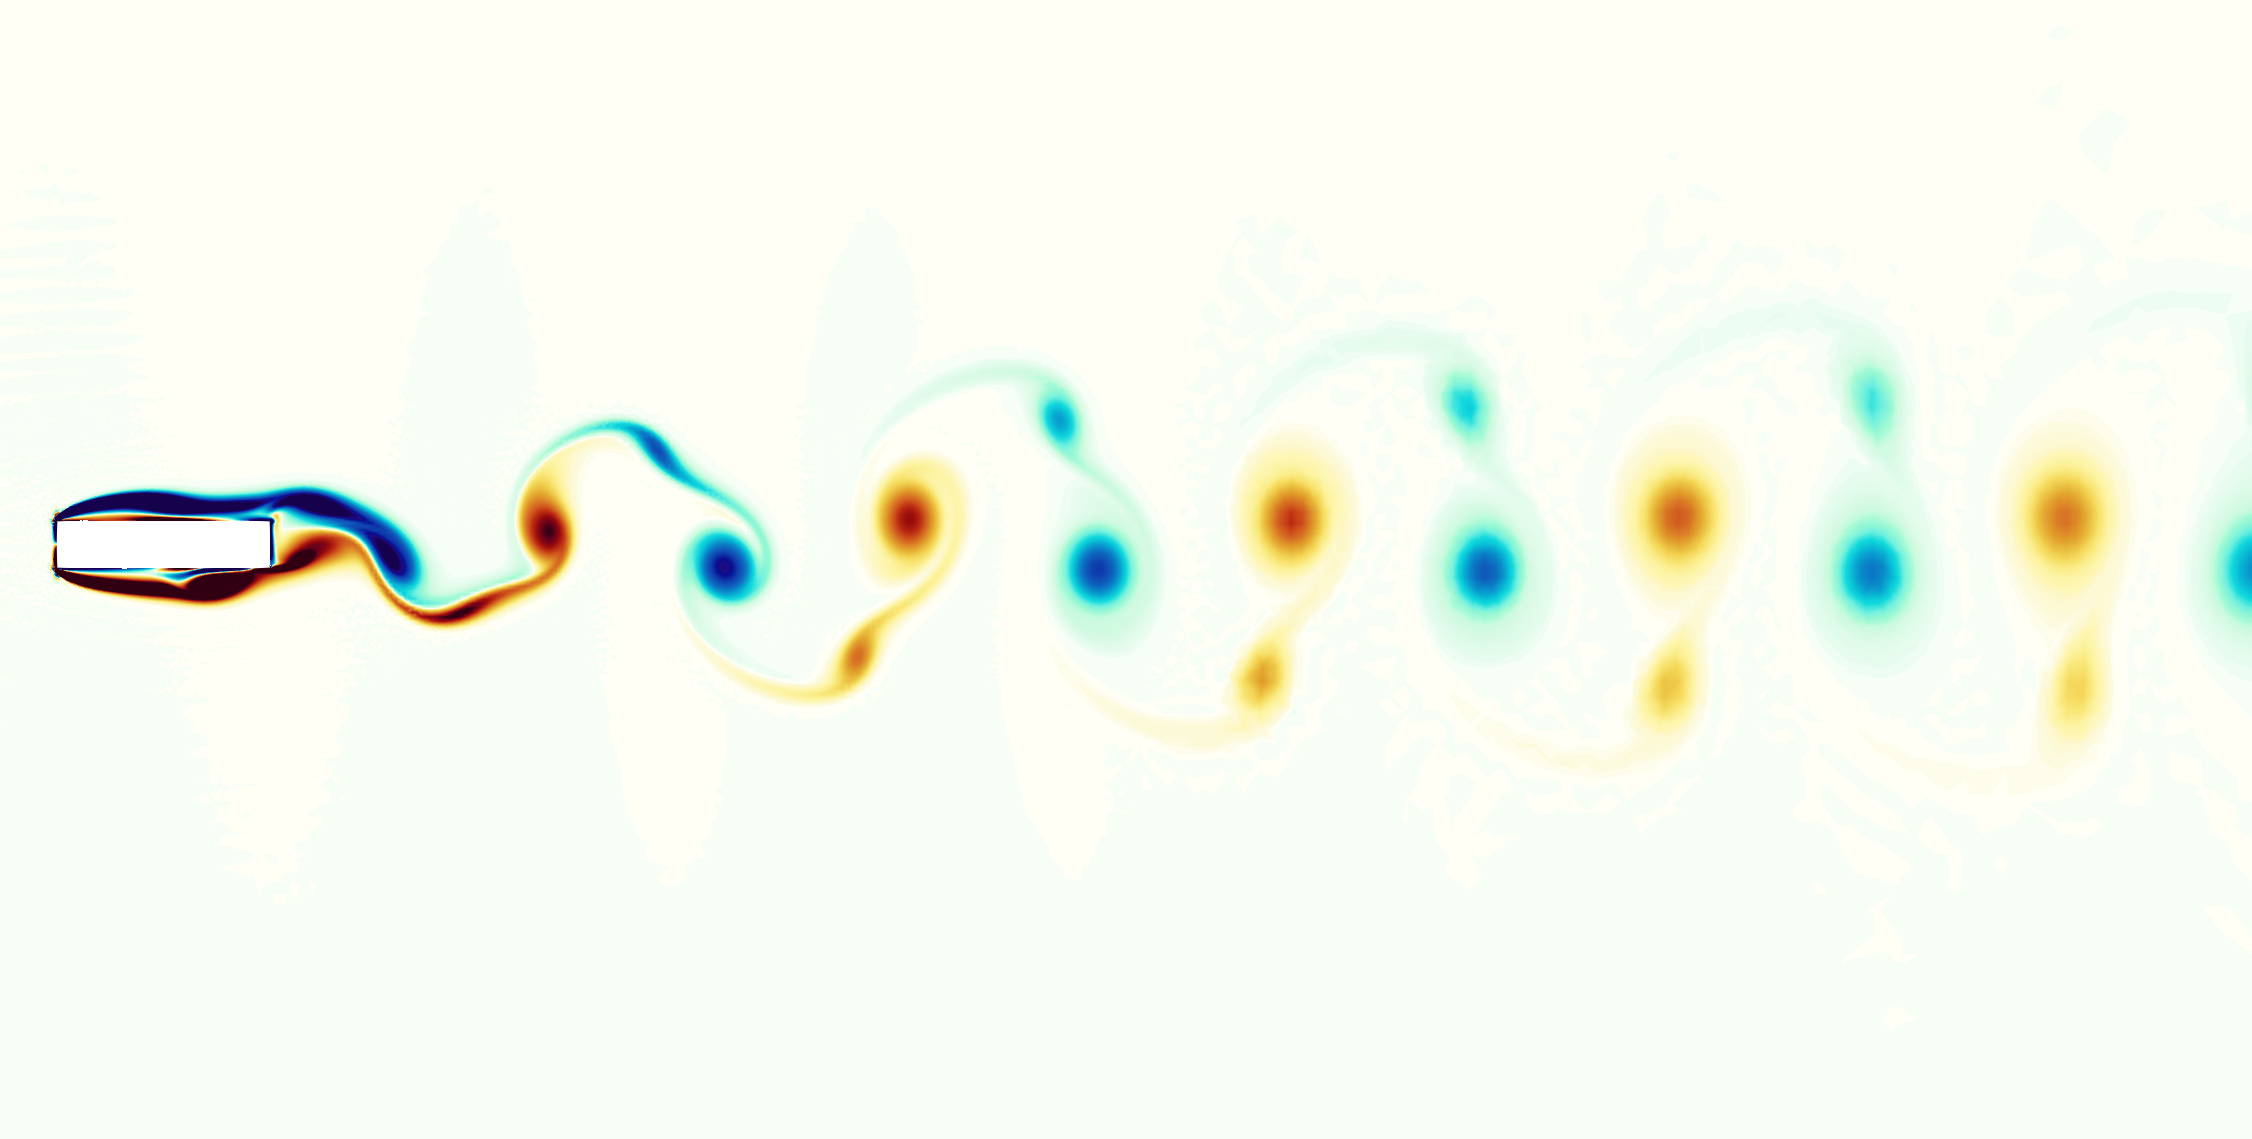
\includegraphics[trim={0 100 0 100},clip,width=0.49\textwidth]{./fig/AR4p5/vort_Re430_75.png}
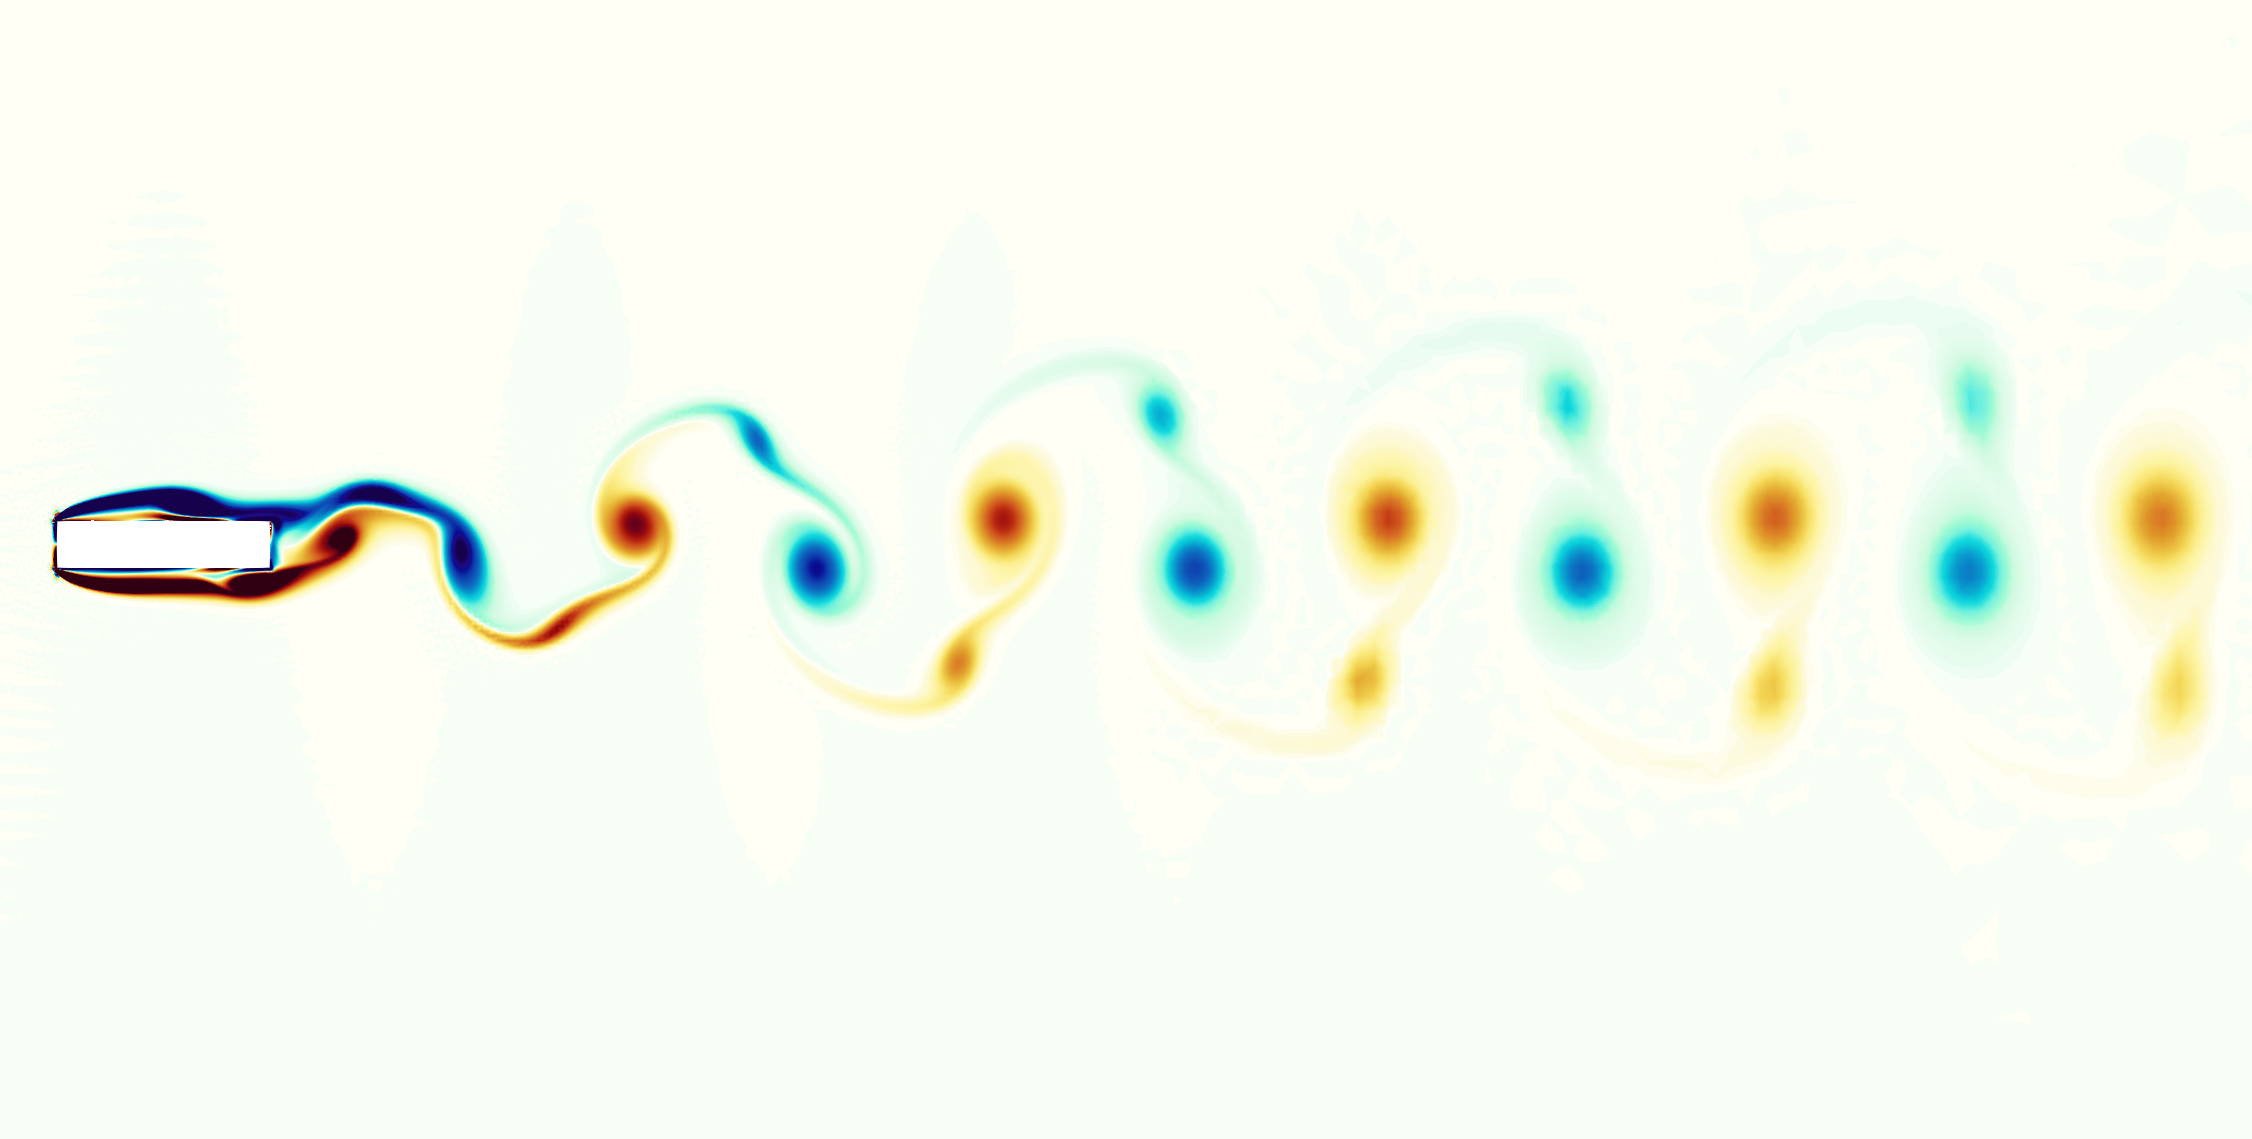
\includegraphics[trim={0 100 0 100},clip,width=0.49\textwidth]{./fig/AR4p5/vort_Re430_100.png}
\vspace{0.1cm}
\begin{tikzpicture}
\draw (-10,2) -- (8,2);
\end{tikzpicture}
\vspace{0.1cm}
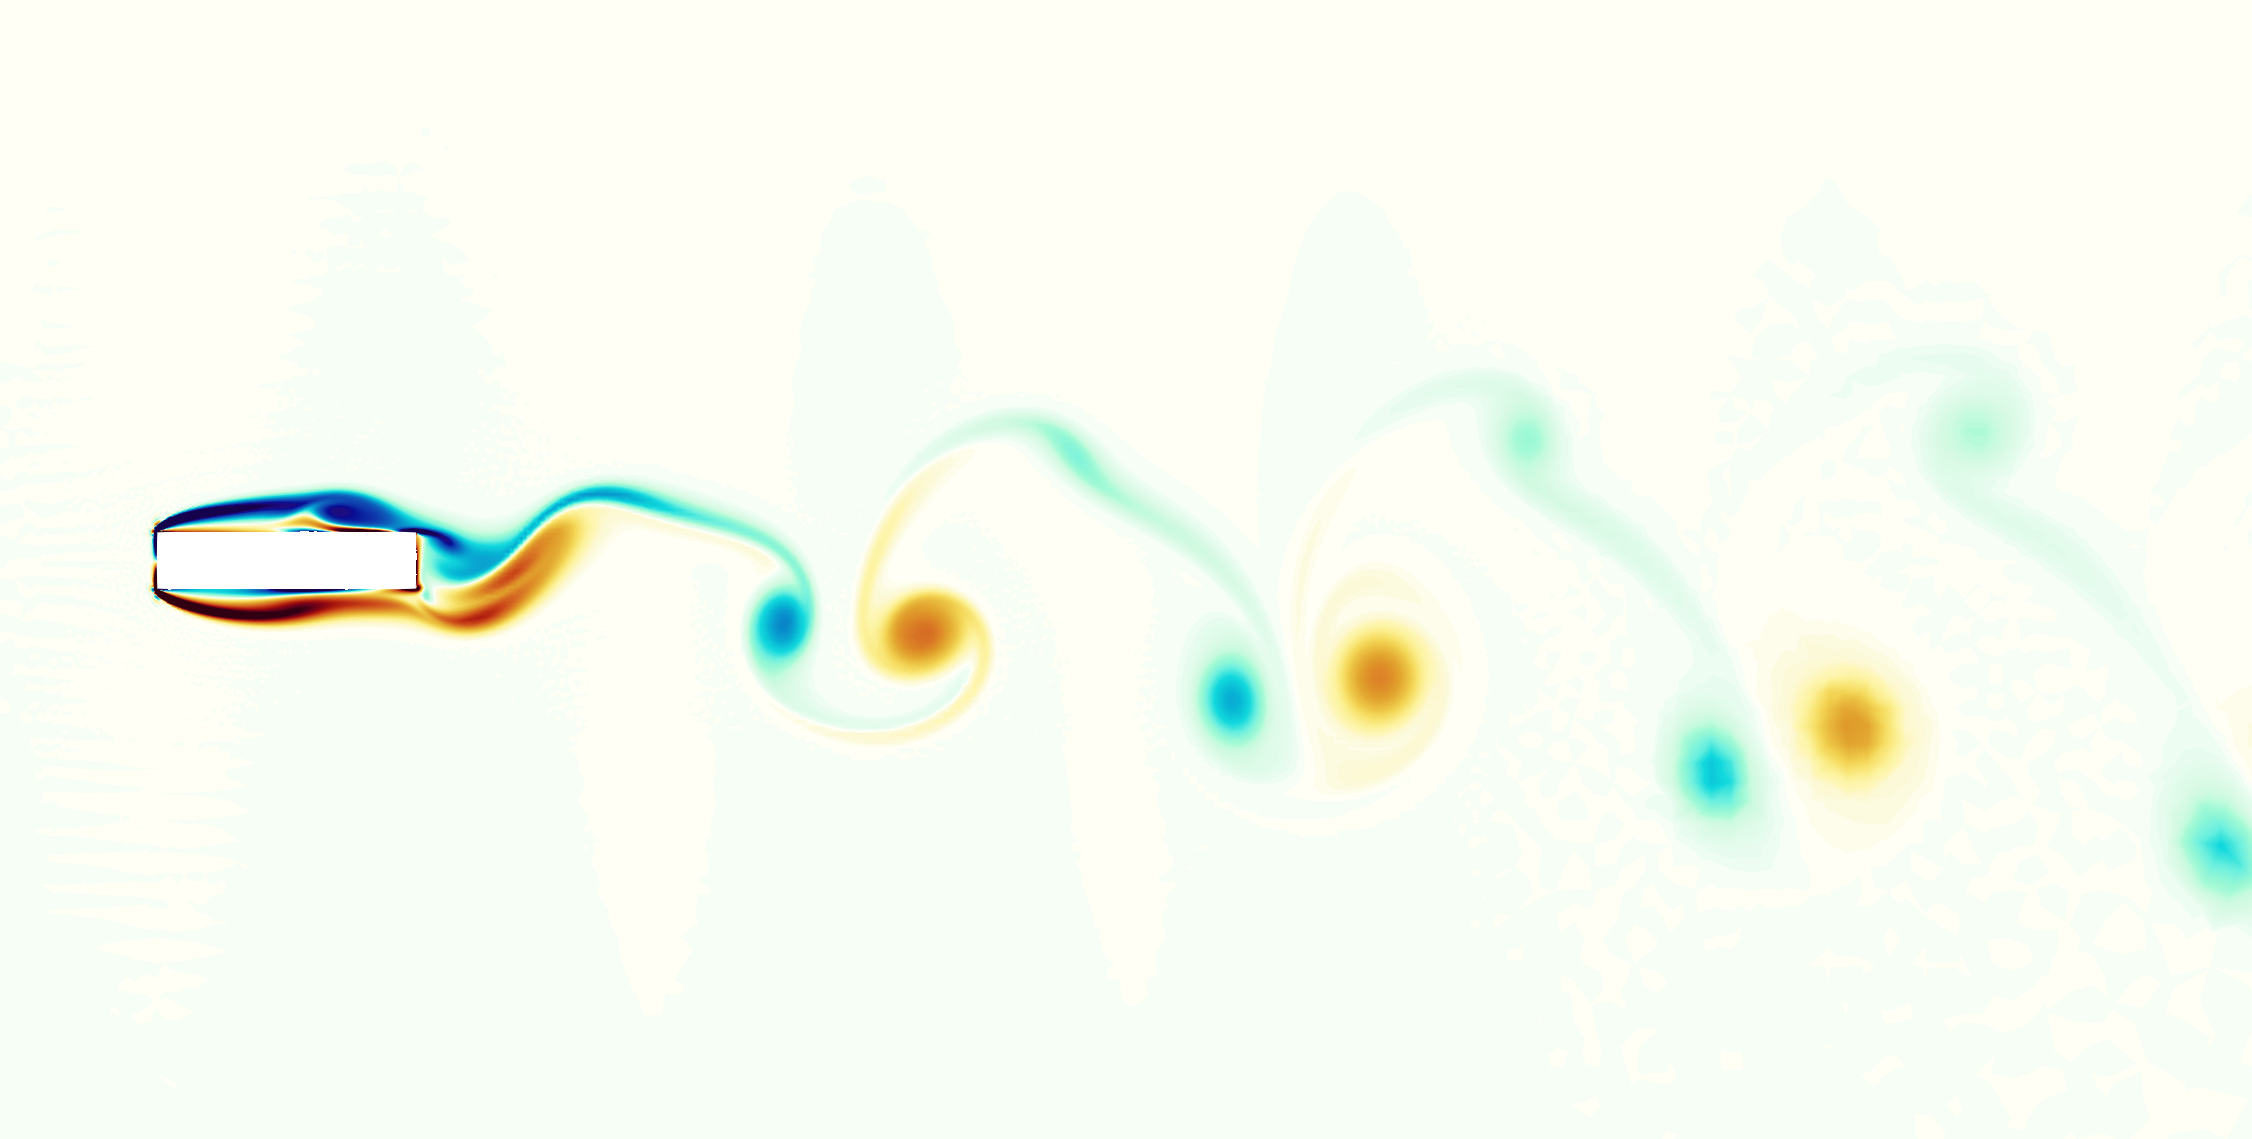
\includegraphics[trim={0 100 0 100},clip,width=0.49\textwidth]{./fig/AR4p5/vort_Re450_25.png}
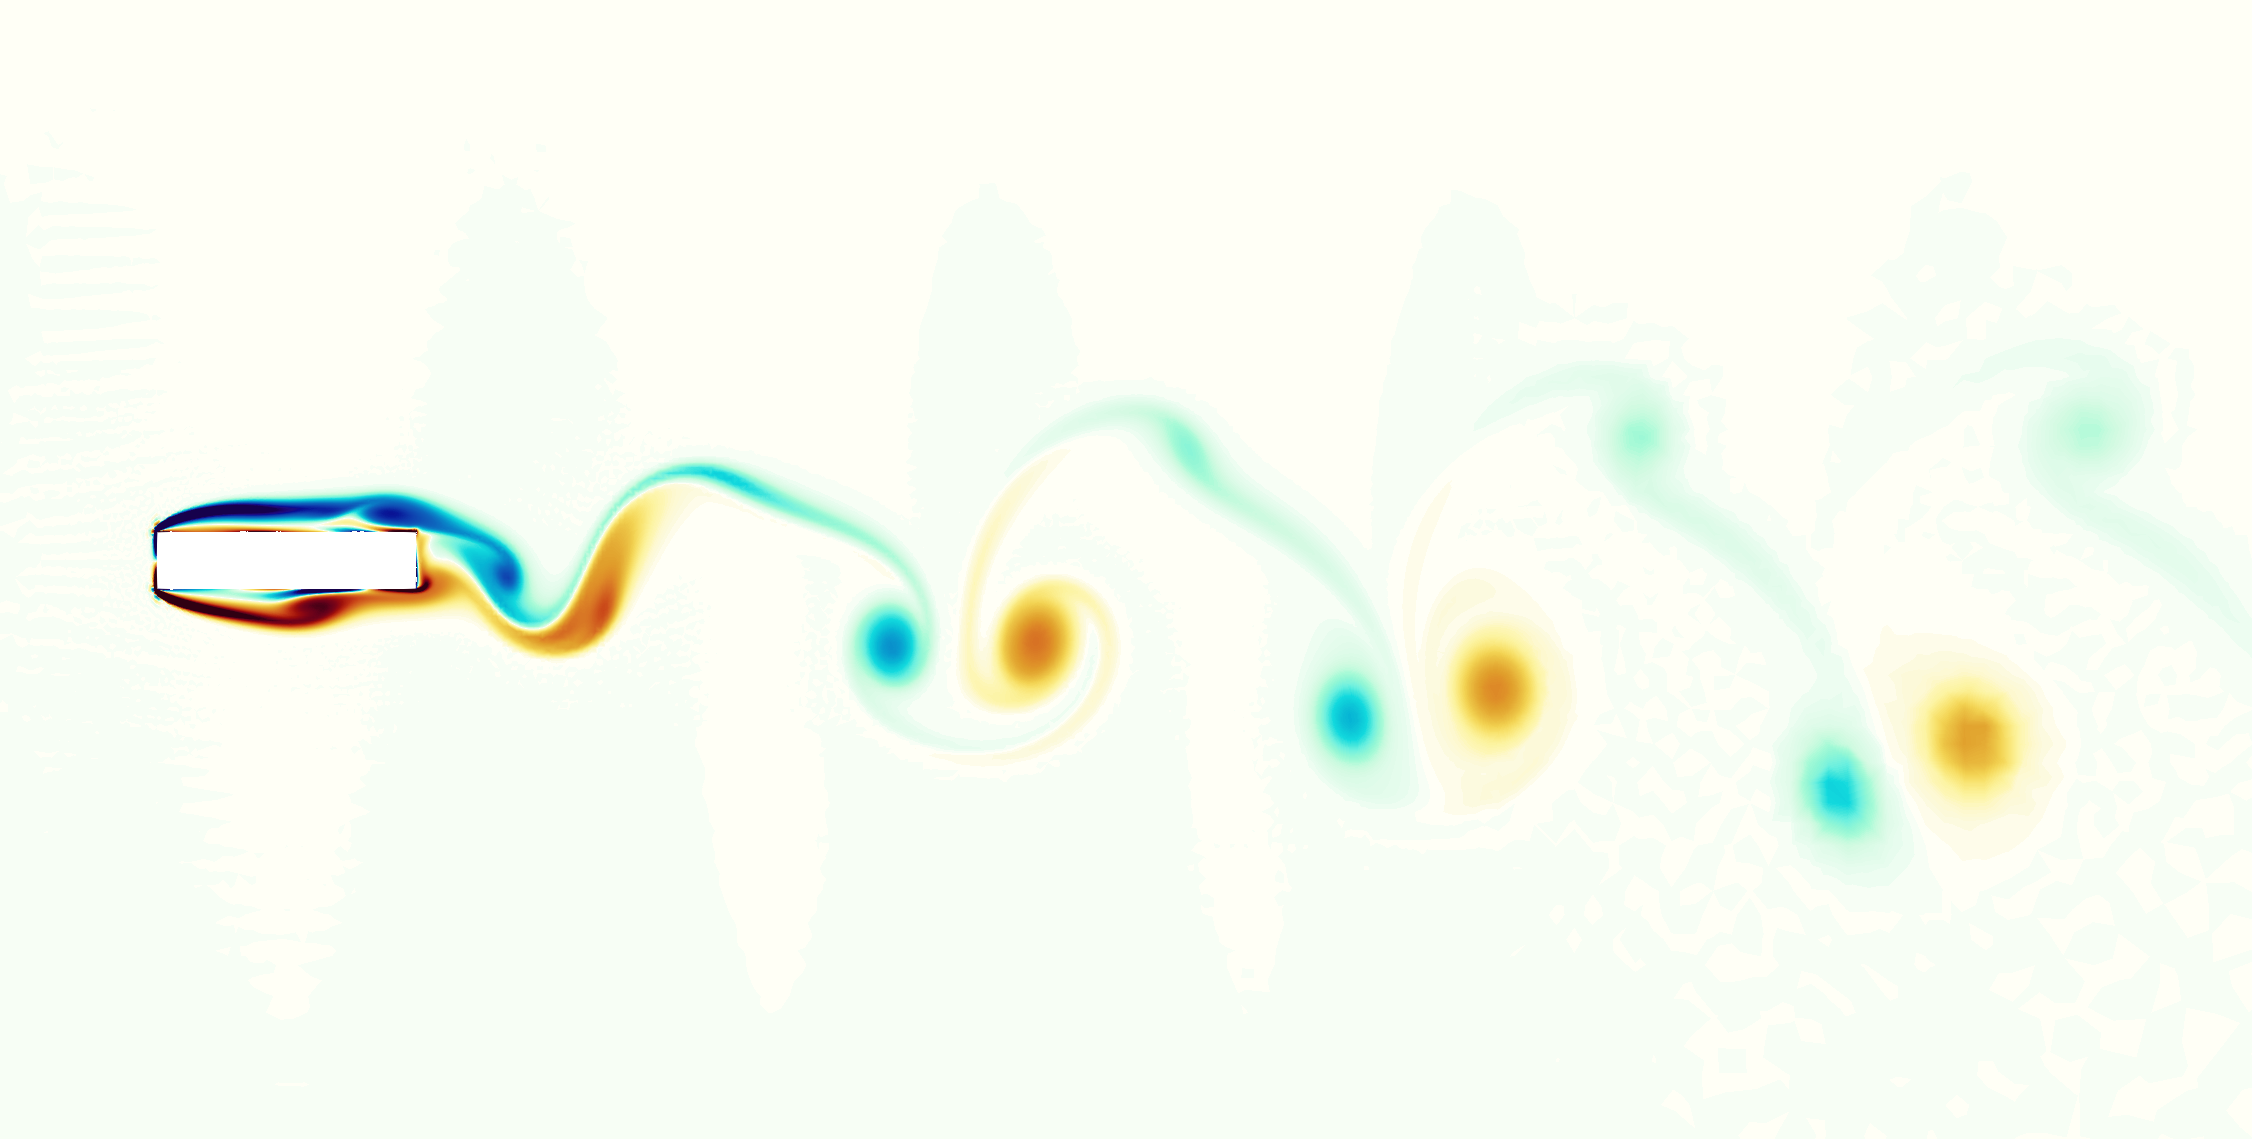
\includegraphics[trim={0 100 0 100},clip,width=0.49\textwidth]{./fig/AR4p5/vort_Re450_50.png}
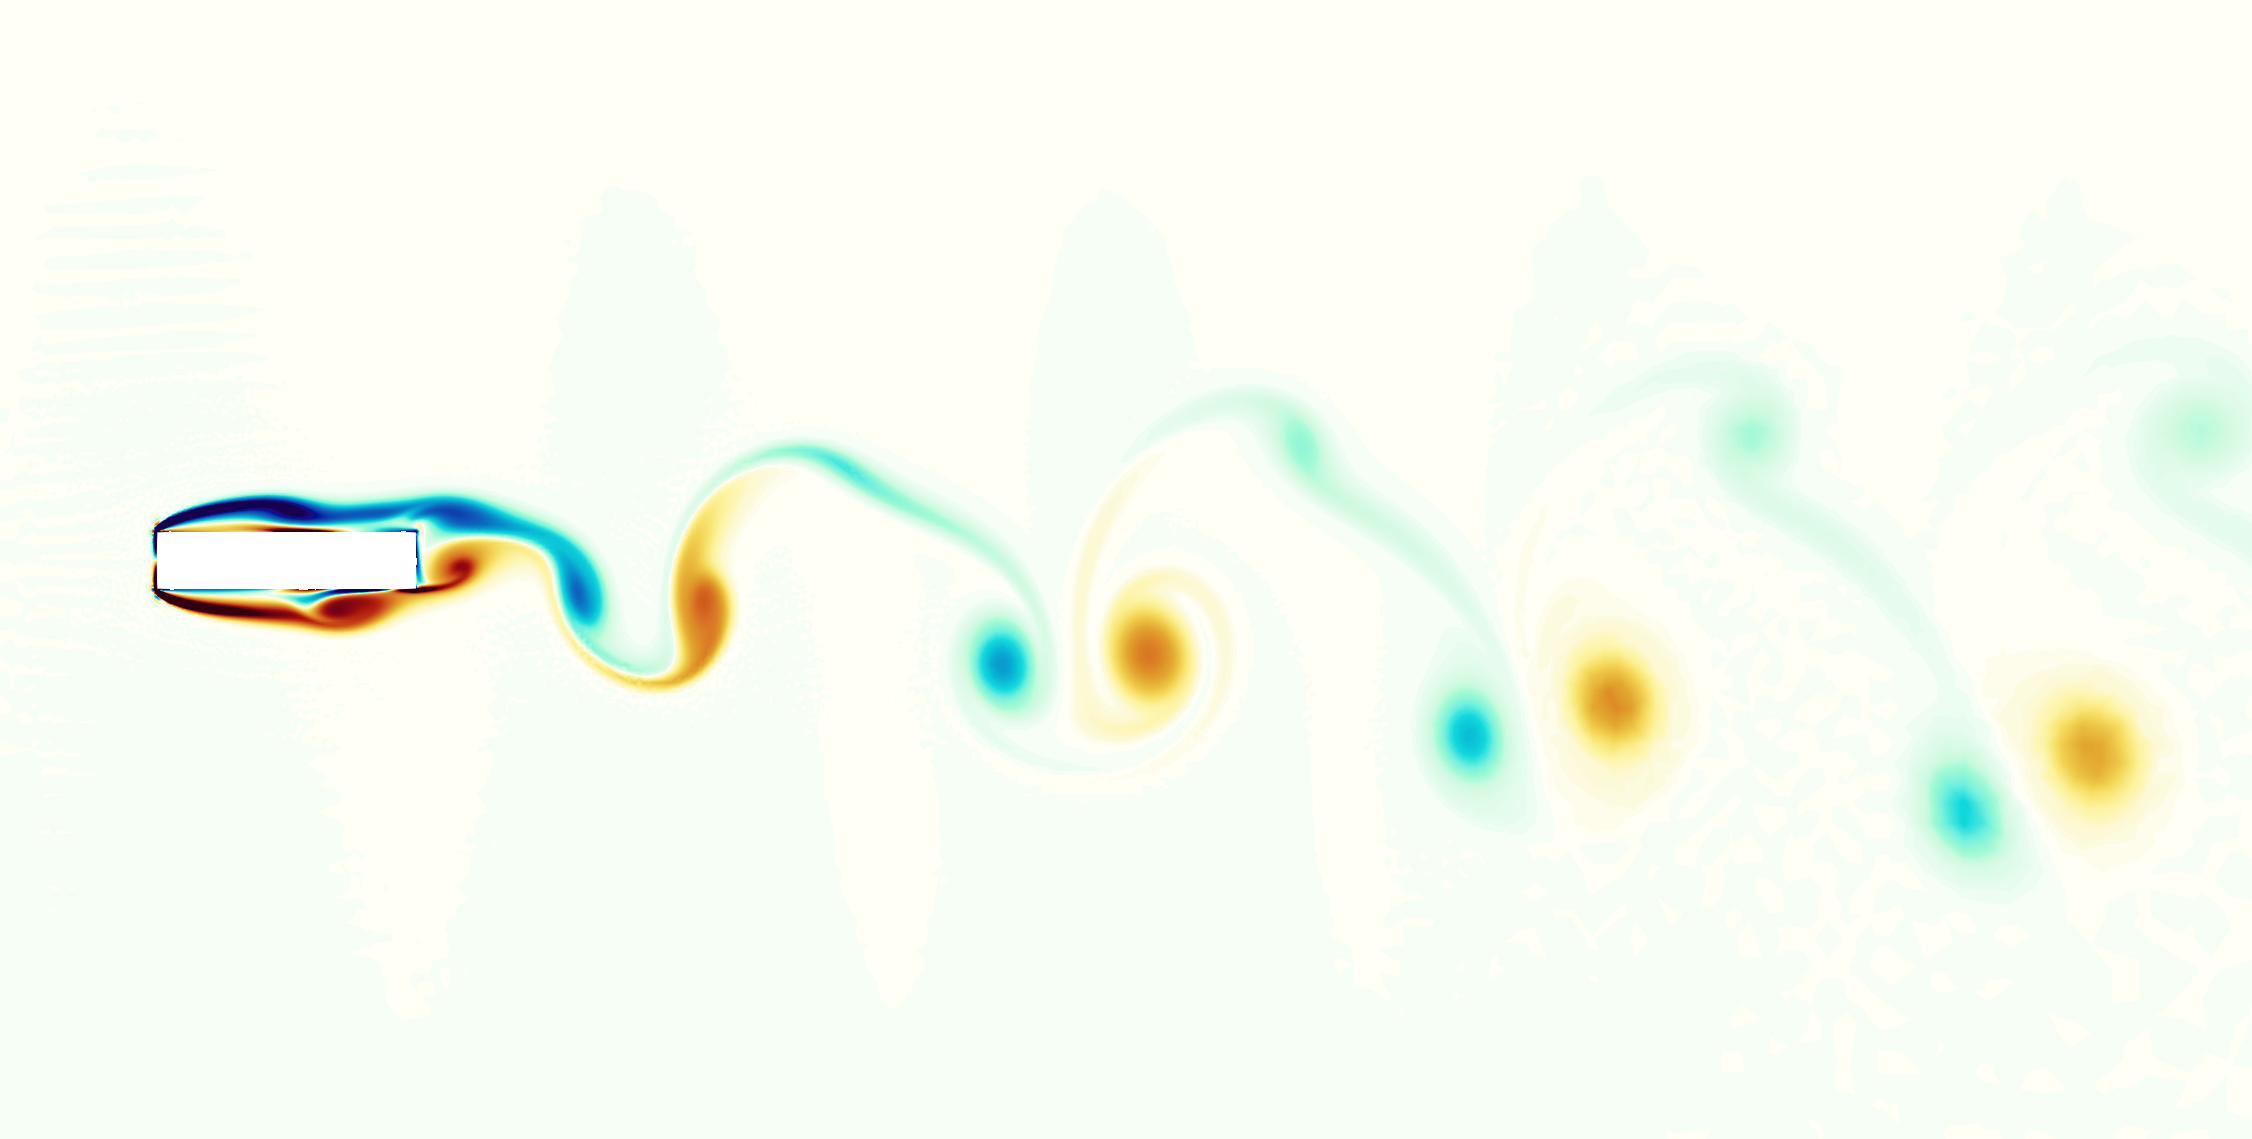
\includegraphics[trim={0 100 0 100},clip,width=0.49\textwidth]{./fig/AR4p5/vort_Re450_75.png}
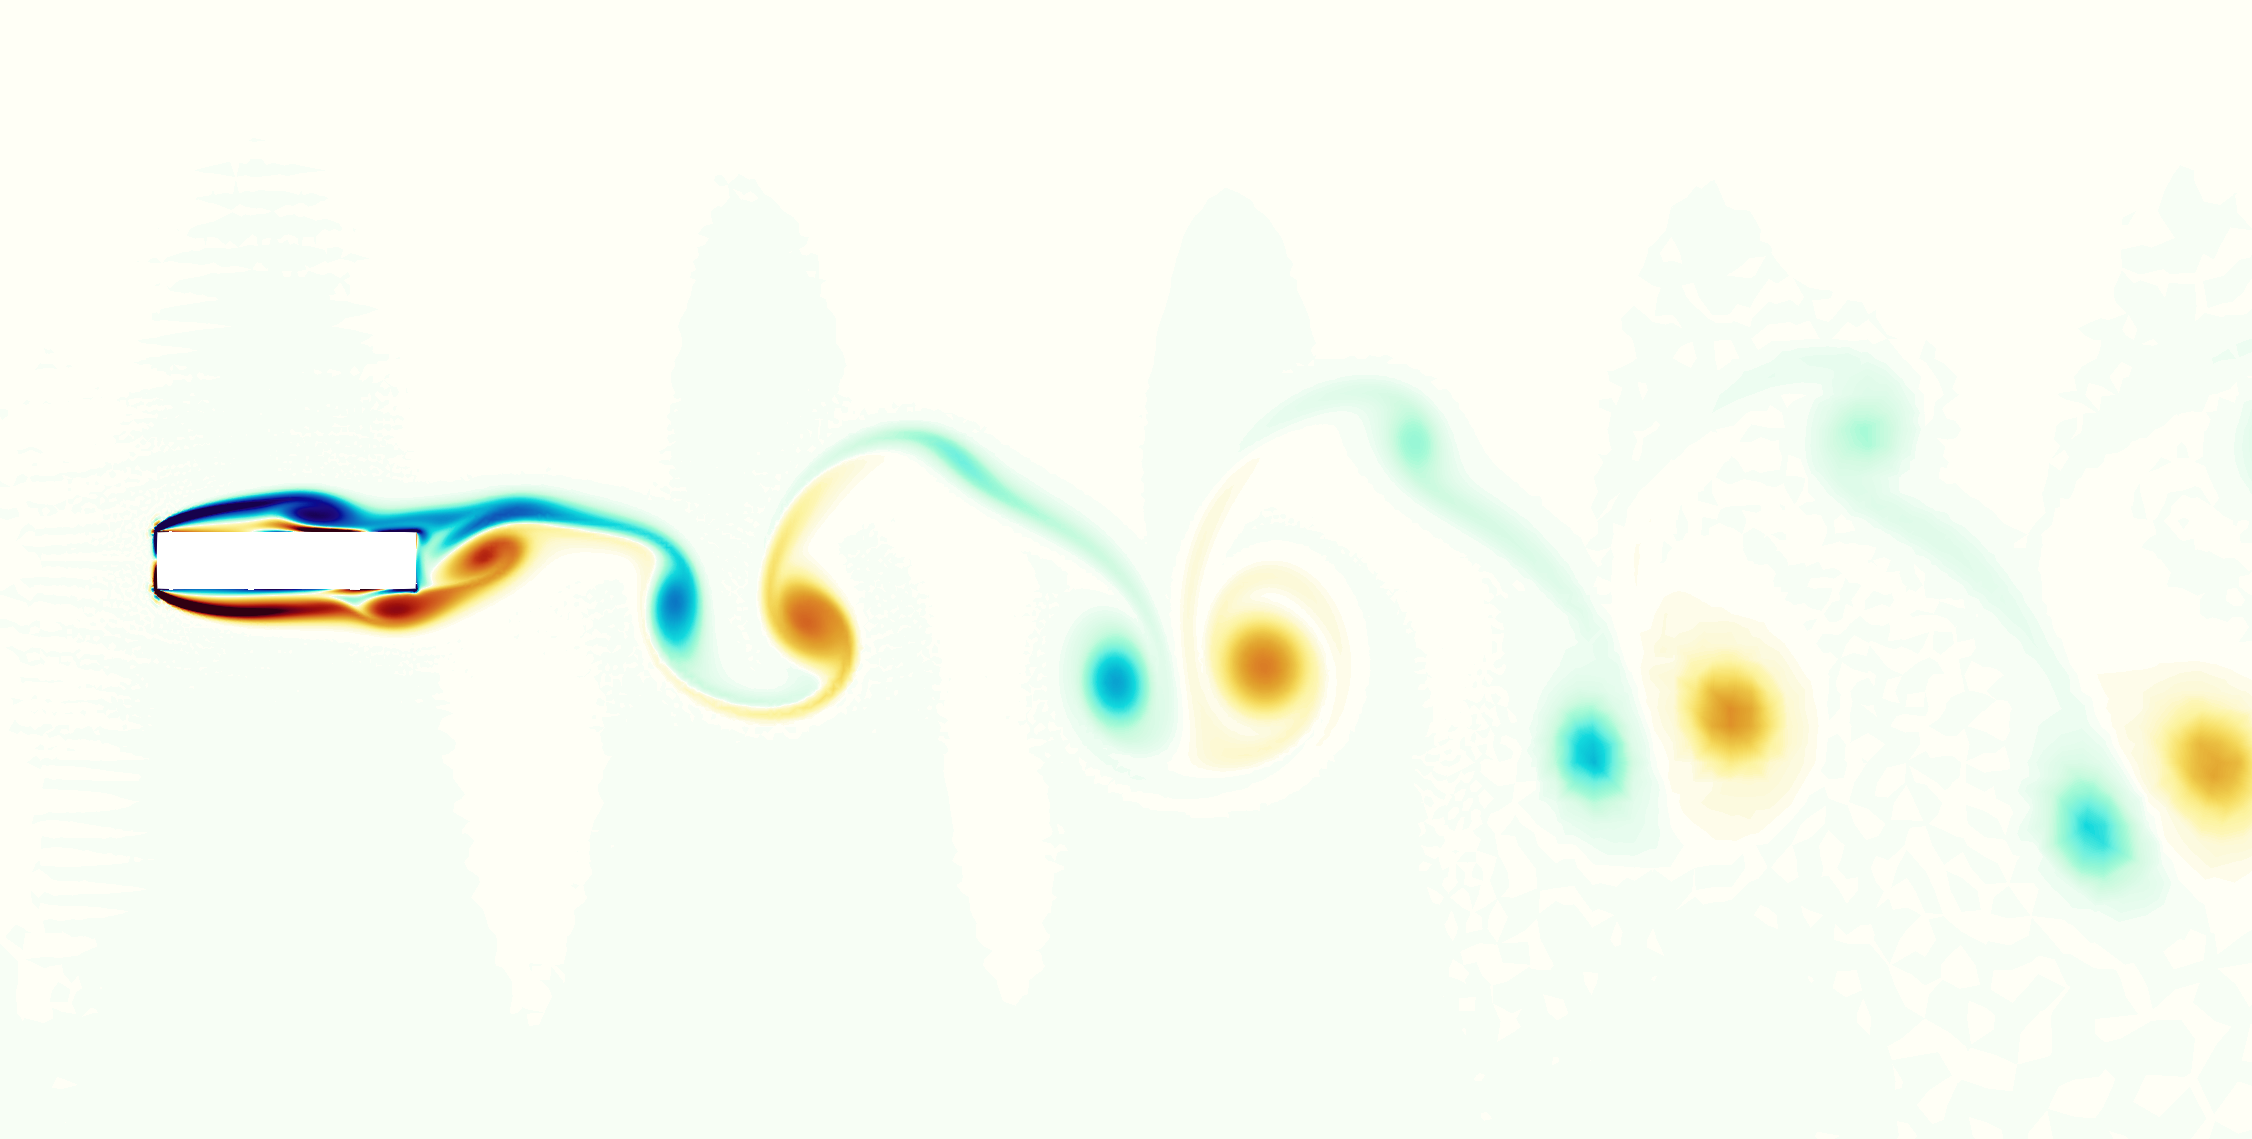
\includegraphics[trim={0 100 0 100},clip,width=0.49\textwidth]{./fig/AR4p5/vort_Re450_100.png}
\caption{Top: Evolution of the vorticity in one oscillation period for $\AR=4.5$ and $Re=430$. Bottom: Evolution of the vorticity in one oscillation period for $\AR=4.5$ and $Re=450$.}
\label{fig:vort_AR4p5_Re450}
\end{figure}

\begin{figure}
\centering
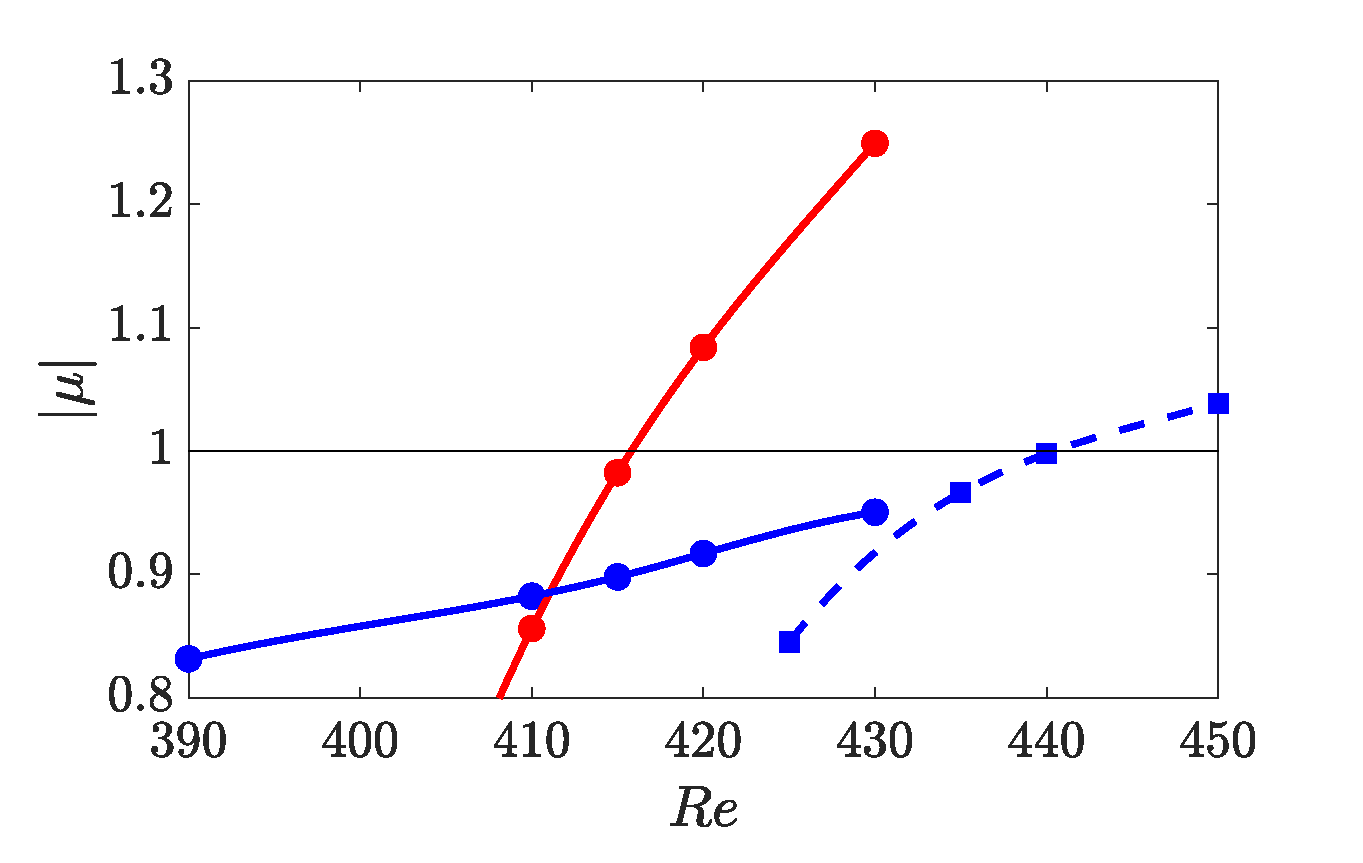
\includegraphics[width=0.49\textwidth]{./fig/AR4p5/multipliers_2D.eps}
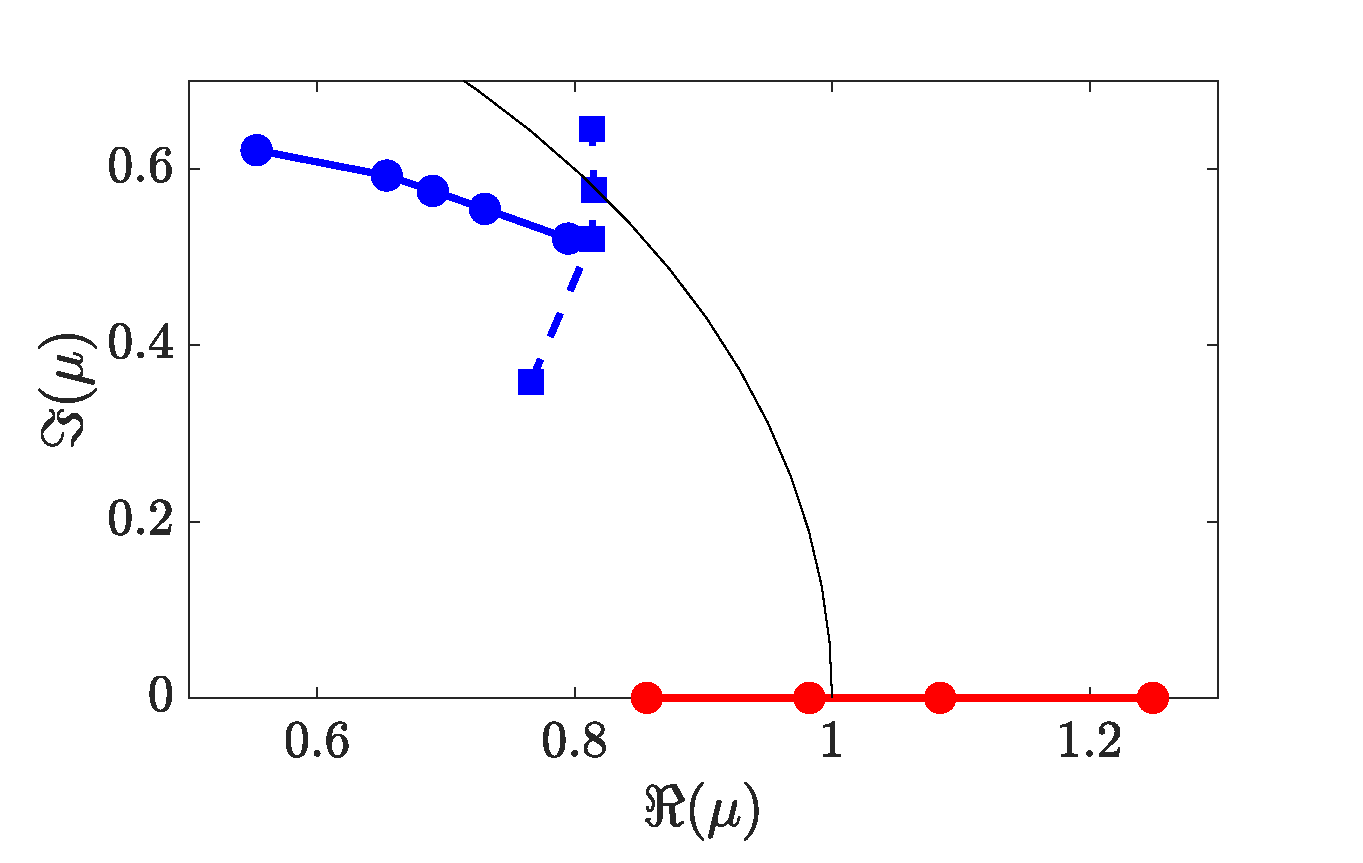
\includegraphics[width=0.49\textwidth]{./fig/AR4p5/multipliers_2D_b.eps}
\vspace{0.1cm}
\begin{tikzpicture}
\draw (-10,2) -- (8,2);
\end{tikzpicture}
\vspace{0.1cm}
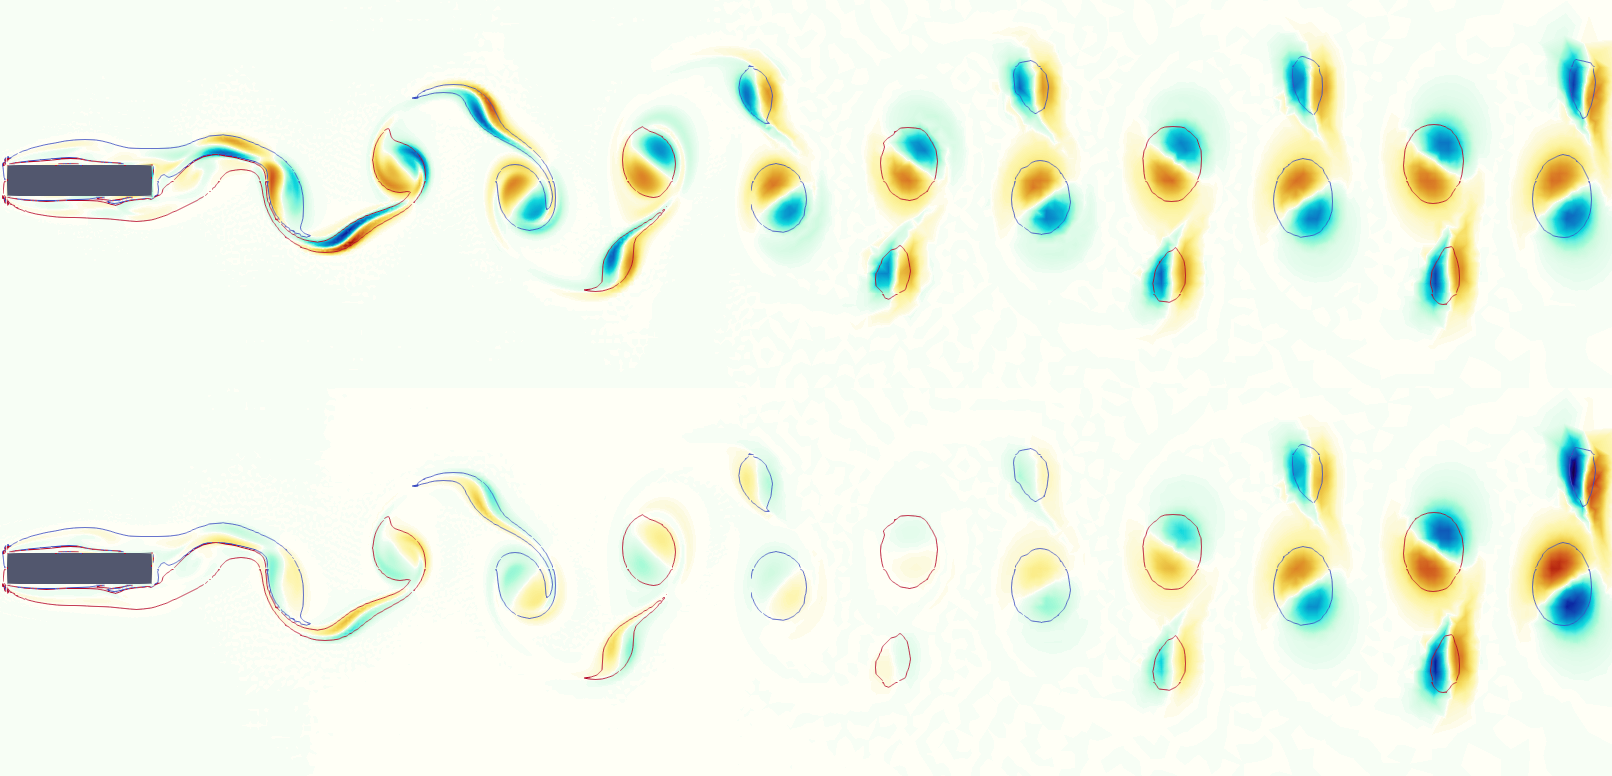
\includegraphics[width=0.7\textwidth]{./fig/AR4p5/omegaz_beta0_Re430_AB.png}
\vspace{0.1cm}
\begin{tikzpicture}
\draw (-10,2) -- (8,2);
\end{tikzpicture}
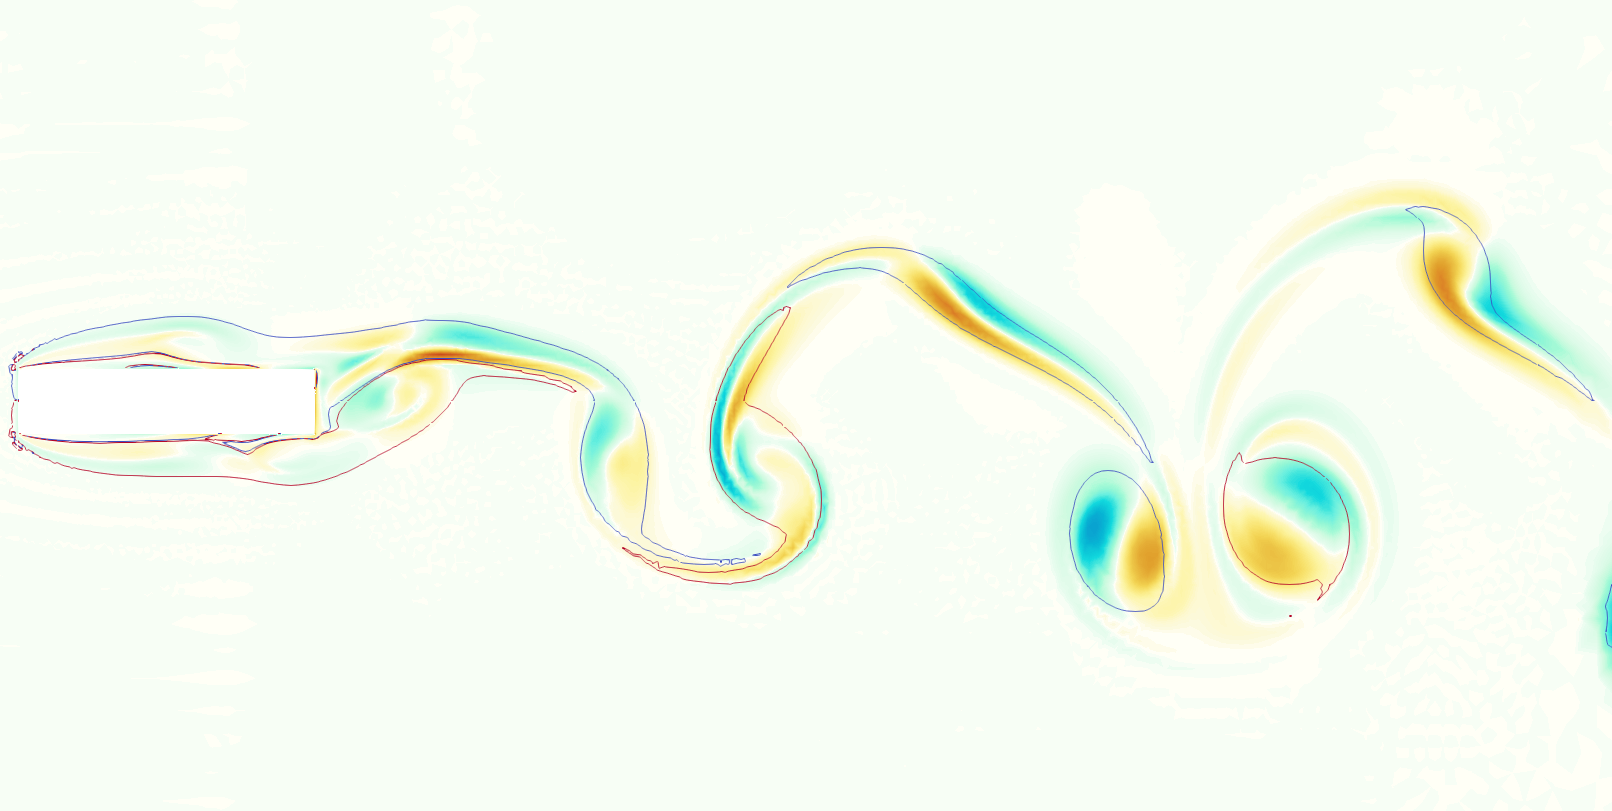
\includegraphics[width=0.7\textwidth]{./fig/AR4p5/Floqetmode_beta_0_Re450_AR4p5.png}
\caption{$2D$ bifurcation of the periodic flow past a rectangular cylinder with $\AR=4.5$. Top: Multipliers associated with the straight (solid) and slanted (dashed) wake for $\AR=4.5$. The left panel plots $|\mu|$ as a function of $\beta$. The red colour refers to real and positive multipliers, while the blue colour refer to complex mutlpliers. The right panel shows the dependence of $\Re(\mu)$ and $\Im(\mu)$ on $Re$. Note that the slanted wake is the results of the synchronous instability described by the red branch. Once the wake becomes slanted a new branch with complex conjugate multipliers arises that becomes unstable at $Re \approx 450$. Centre: Floquet modes associated with the straight wake; the colours are for the spanwise vorticity and the above and bottom panel refer to the red and blue branches respectively. Bottom: Floquet mode associated with the blue branch of the slanted wake.}
\label{fig:AR4p5_modes_Re430_beta0}
\end{figure}

\begin{figure}
  \centering
  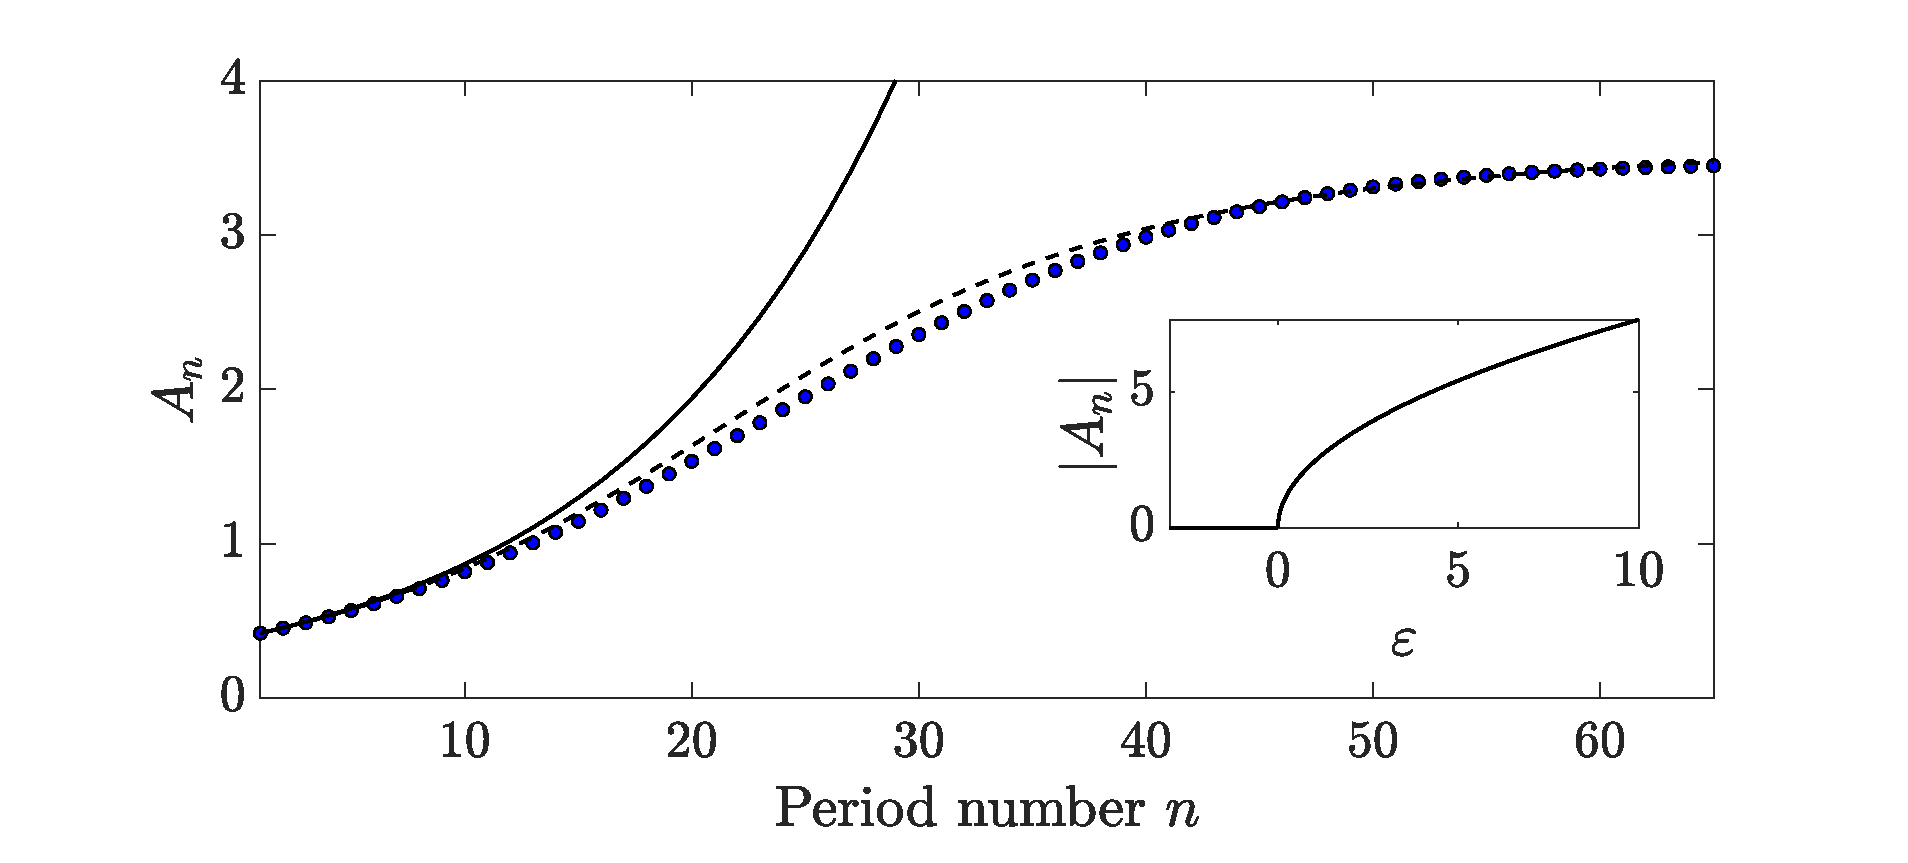
\includegraphics[width=0.7\textwidth]{./fig/AR4p5/Nlgrowth_Re420.eps}
  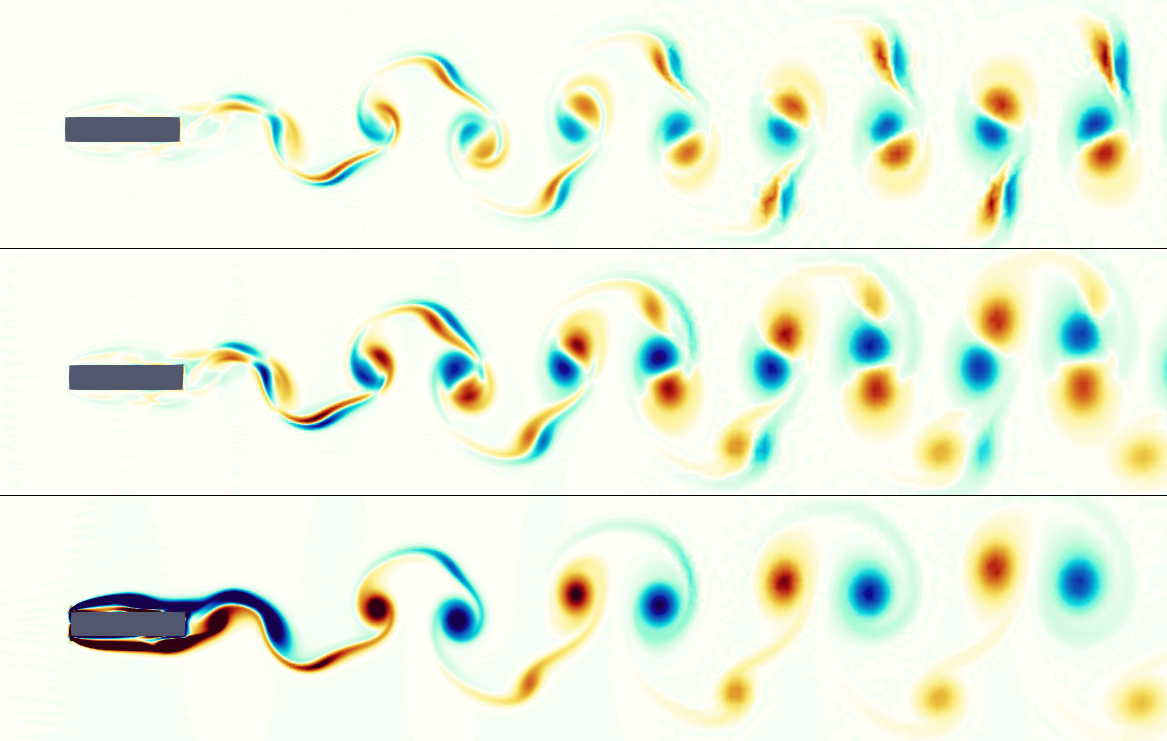
\includegraphics[width=0.8\textwidth]{./fig/AR4p5/LinNonLin_Re420.png}
  \caption{Nonlinear growth of the 2D perturbation to the wake near the secondary instability threshold for $\AR=4.5$ and $Re=420$. Top: the blue circles are the amplitude of $A_n$ evaluated from simulations of the full Navier--Stokes equations at $Re=420$. The solid line shows the prediction $A_{n+1} = \mu A_n$, while the dashed line shows the prediction $A_{n+1} = ( \mu + \alpha_1 A_n + \alpha_2 A_n^3 ) A_n$, with $\alpha_1 = -0.01114$ and $\alpha_2 = 0.000359$. The inset shows the bifurcation diagram. Bottom: snapshots of the vorticity field for linear and nonlinear perturbations and of the total field.}
\end{figure}

\begin{figure}
\centering
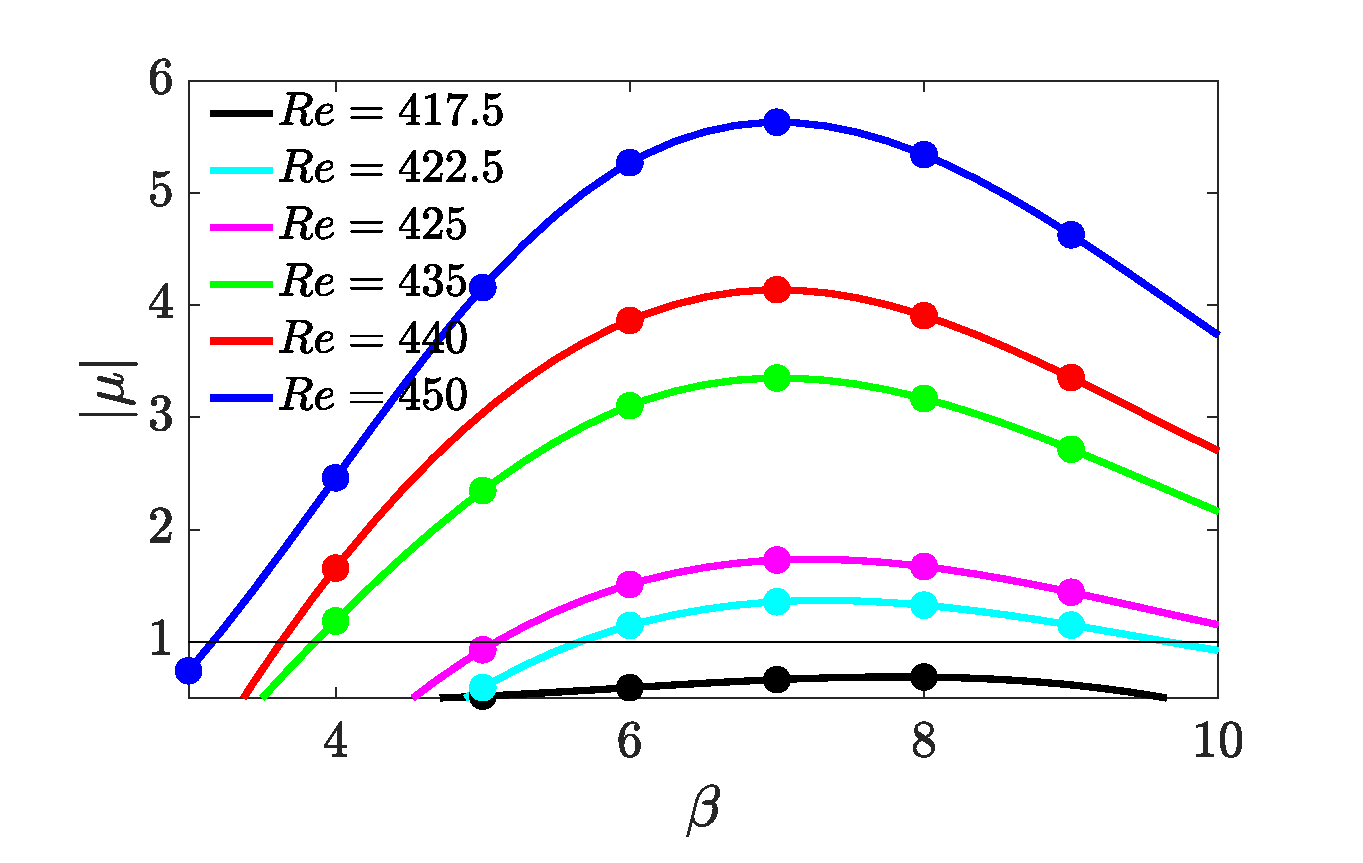
\includegraphics[width=0.49\textwidth]{./fig/AR4p5/multipliers_3D.eps}
\vspace{0.1cm}
\begin{tikzpicture}
\draw (-10,2) -- (8,2);
\end{tikzpicture}
\vspace{0.1cm}
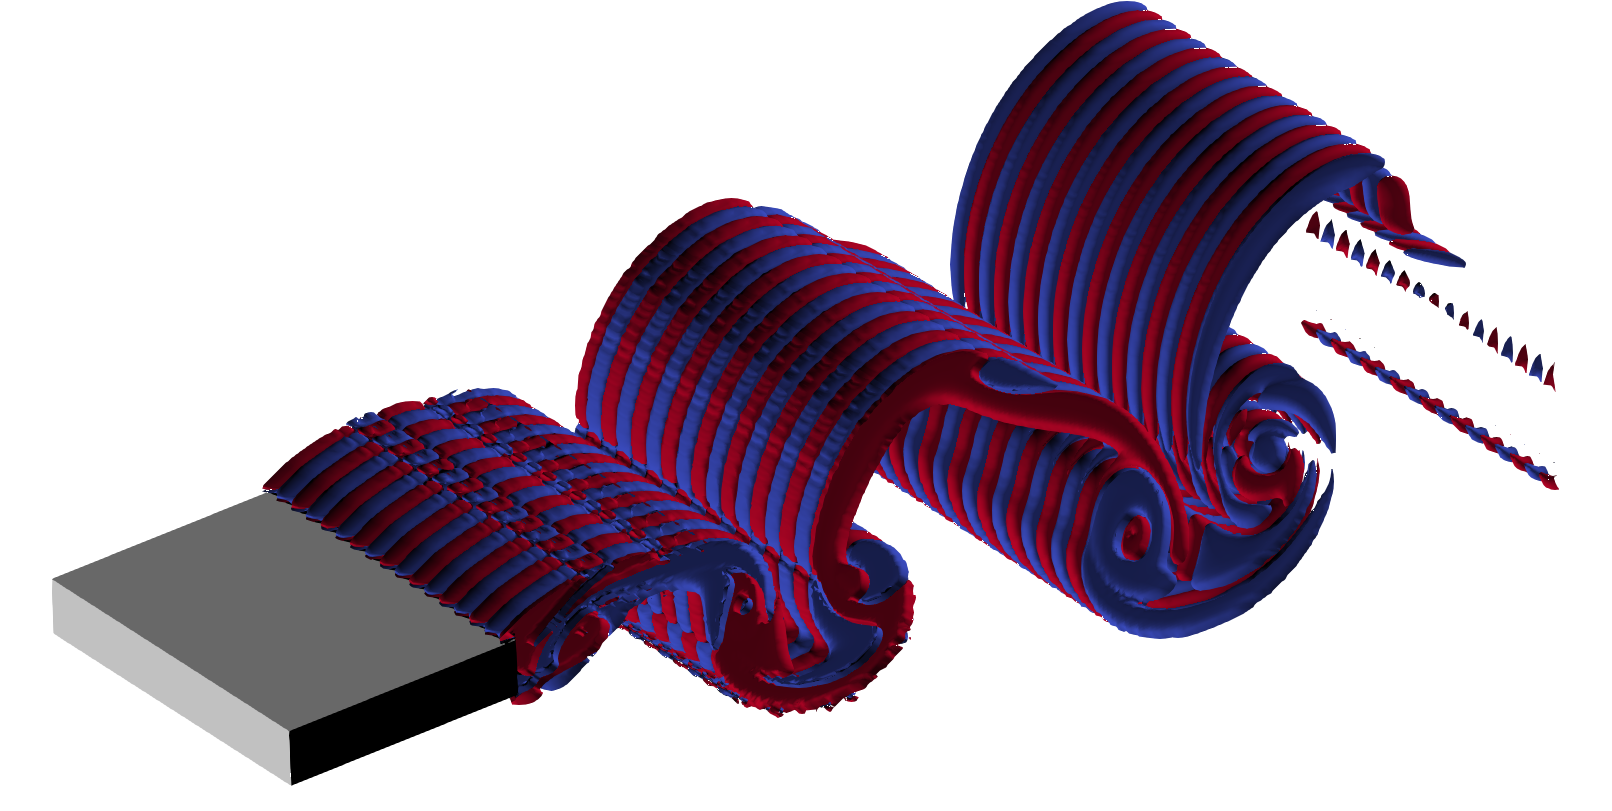
\includegraphics[trim={0 0 0 0},clip,width=0.49\textwidth]{./fig/AR4p5/Floqetmode_beta_8_Re450_AR4p5.png}
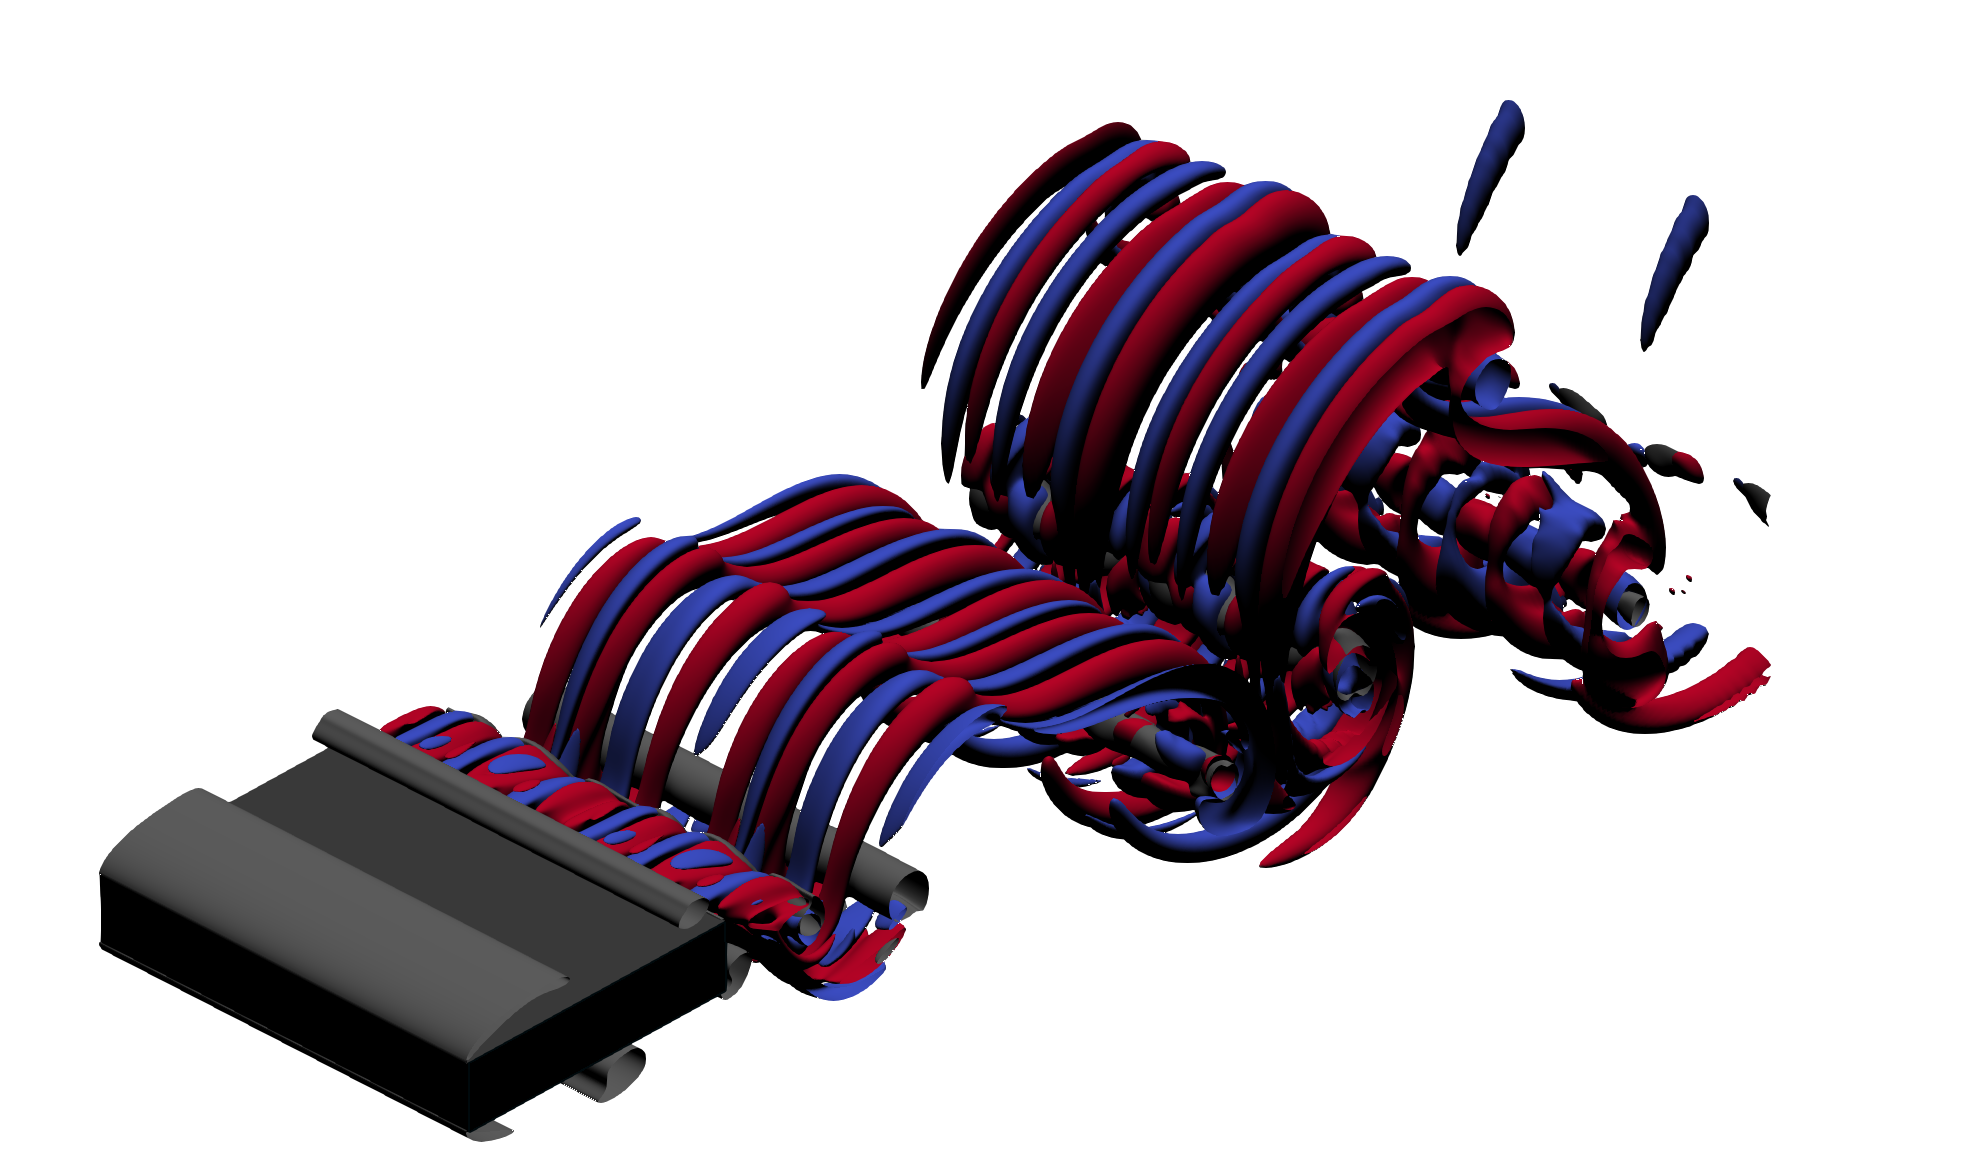
\includegraphics[width=0.49\textwidth]{./fig/AR4p5/lambda2_omegax-3D-Re450b.png}
\caption{Three-dimensional instability of the flow past a rectangular cylinder with $\AR=4.5$. The flow become unstable once the wake has bifurcated to a slanted configuration. The resulting limit cycle is (strongly) unstable to three-dimnsional perturbation of subharmonic nature (here the multipliers are real and negative); see top panel. Modes from the Floquet analysis for $\AR=4.5$. Bottom: Imaginary part of the streamwise vorticity for $\AR=4.5$, $Re=450$ and $\beta=8$ associated with the unstable subharmonic multiplier. Bottom right: DNS of the flow past the rectangular cylinder with $\AR=4.5$ at $Re=450$. Red/blue isosurfaces indicate $\omega_x = \pm 0.015$. Note that the wake is slanted and three-dimensional, as predicted by the Floquet stabilty analysis. The spanwise extent of the computational domain is $L_z=2\pi$.This means that the wavenumber associated with the three-dimensionality is $\beta \approx 6$, which is consistent with the most amplified wavenumber detected with the stability analysis.}
\label{fig:AR4p5_modes_Re430_beta0}
\end{figure}


%\begin{figure}
%\centering
%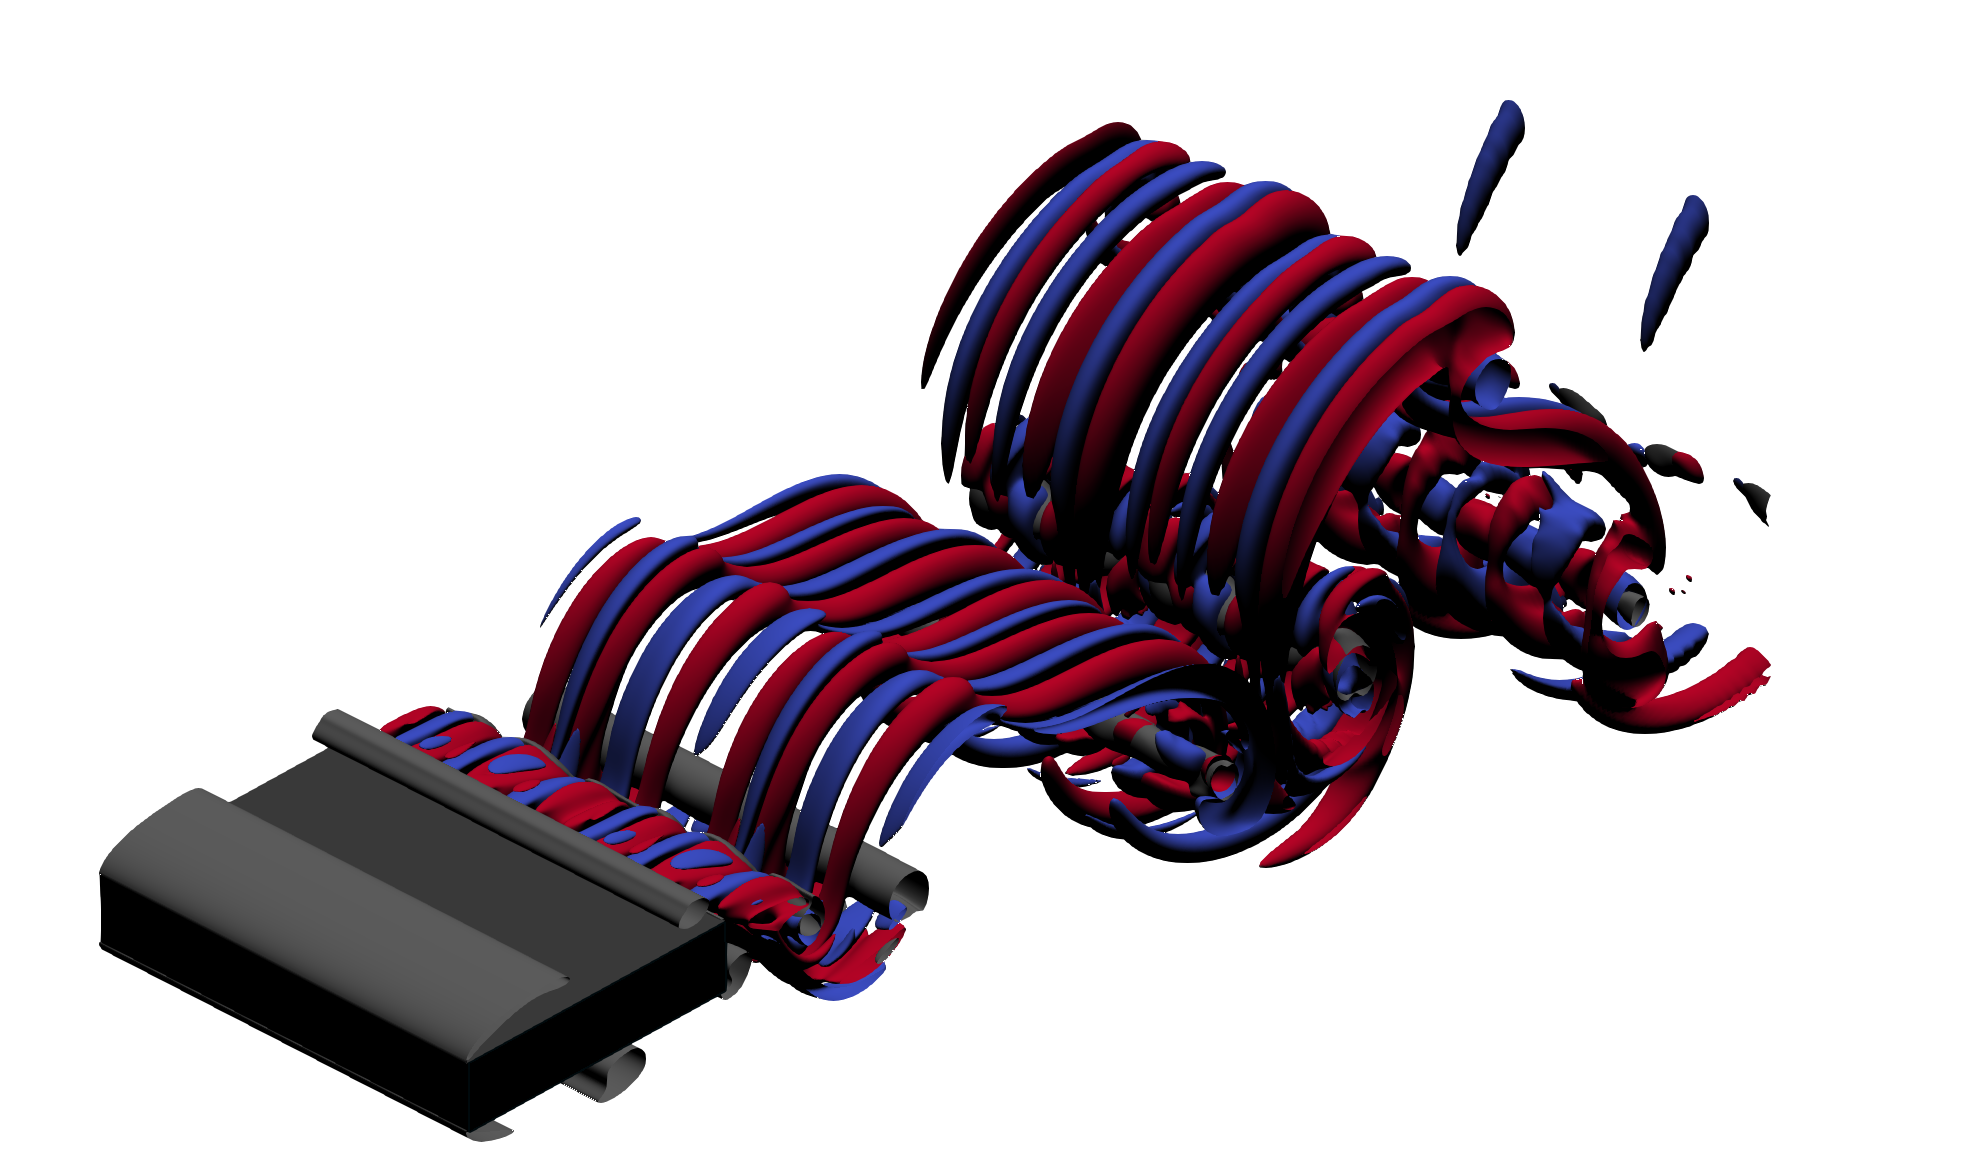
\includegraphics[width=0.7\textwidth]{./fig/AR4p5/lambda2_omegax-3D-Re450b.png}
%\includegraphics[trim=0 200 0 200,width=0.49\textwidth]{./fig/AR4p5/lambda2_omegax-xz-Re450b.png}
%\caption{DNS of the flow past the rectangular cylinder with $\AR=4.5$ at $Re=450$. Red/blue isosurfaces indicate $%\omega_x = \pm 0.015$. Note that the wake is slanted and three-dimensional, as predicted by the Floquet stabilty analysis. The spanwise extent of the computational domain is $L_z=2\pi$.This means that the wavenumber associated with the three-dimensionality is $\beta \approx 6$, which is consistent with the most amplified wavenumber detected with the stability analysis.}
%\label{fig:lambda2_omegax_AR45_Re450}
%\end{figure}



\subsection{Bodies with $5 < \AR < 6$}

\begin{itemize}
  \item Here we look at the second oblique branch of the $St_L-\AR$ plane. Here we have already found that for $\AR=5$ the first mode to become unstable is mode QS, i.e. the quasi-subharmonic mode.
  \item We now investigate what happens when increasing $\AR$. We recall that this is the range where the vortex shedding is dominated by the TE. This means that the dynamics of the TE vortex shedding dominates and is not directly influenced by the vortex shedding from the LE as in the oblique branches. As shown in figure \ref{fig:mult_AR5s}, for $\AR=5$ the only unstable mode is of subharmonic nature and is the so-called mode $QS$. As $\AR$ is increased, instead, a new mode of synchronous nature appears (in this case the multipliers are real and positive). For $\AR=5.25$ this mode is stable. For $\AR=5.35$ this mode approaches the unit circle. For $\AR=5.5$ this mode is unstable, and its growth rate is larger than the corresponding one associated with mode $QS$. The second mode here detected resembles mode $A$ for the wake past short cylinders. 
  \item Mode QS is an unstable mode of the recirculating region along the lateral sides of the cylinder. This is visualised in figure \ref{fig:mult_AR5s} (note that the mote is maximum there and not in the wake). For additional details see \citep{chiarini-etal-2022}. The synchronous mode, instead, is an unsteady mode of the wake and share several properties with the classical mode $A$ of the circular cylinder.
  \item For the arise of the new mode $A$ in the $5.25 \le \AR \le 5.75$ regime look at the works by Aleksyuk \& Heil (2023) and Aleksyuk \& Heil (2024). To answer the question "Why this mode is not detected for $\AR=5$? Why it becomes unstable only at larger $\AR$?" We can start looking whether also in this case the mechanism proposed by Aleksyuk \& Heil (2023,2024) works. If this is the case, we can see if for $\AR=5$ we actually have something different. 
\end{itemize}

%For the arise of the new mode $A$ in the $5.25 \le \AR \le 5.75$ regime look at the works by Aleksyuk \& Heil (2023) and Aleksyuk \& Heil (2024)


\begin{figure}
  \centering
%  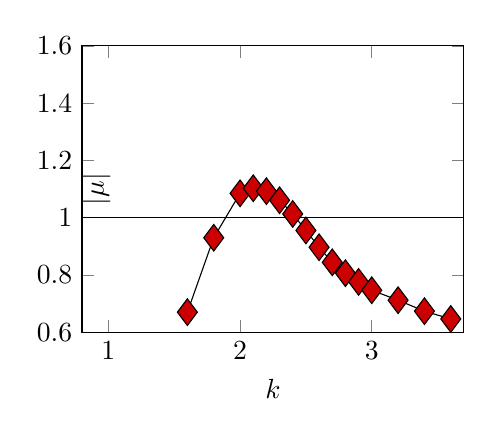
\begin{tikzpicture}



\begin{axis}[%
%width=4.3cm,
%height=3.5cm,
width=0.4\textwidth,
height=0.3\textwidth,
%width=0.2\textwidth,
%height=0.2\textwidth,
scale only axis,
%grid=both,
%axis lines=middle,
xmin=0.8,
xmax=3.7,
ymin=0.6,
ymax=1.6,
%xtick={2, 3, 4, 5, 6, 7, 8, 9, 10, 11},
%ytick={2, 2.5, 3, 3.5, 4, 4.5, 5, 5.5, 6, 6.5, 7},
%xlabel style={font=\color{white!15!black}},
xlabel={$k$},
ylabel={$|\mu|$},
ylabel style={at={(0.1,0.5)}},
%ymin=0,
%ymax=200,
axis background/.style={fill=white},
legend style={at={(0.99,0.85)}, anchor=east, legend cell align=left, align=left, fill=none, draw=none}
]


\addplot [color=black,solid,mark=diamond*,mark options={scale=2.4,black,fill=red!80!black}]
  table[row sep=crcr]{%
   %1.000000000000000   1.000070000000000 \\
  % 1.300000000000000   0.714343000000000 \\
   1.600000000000000   0.670046000000000 \\
   1.800000000000000   0.929885000000000 \\
   2.000000000000000   1.085060000000000 \\
   2.100000000000000   1.102700000000000 \\
   2.200000000000000   1.092560000000000 \\
   2.300000000000000   1.060710000000000 \\
   2.400000000000000   1.012990000000000 \\
   2.500000000000000   0.955412000000000 \\
   2.600000000000000   0.896718000000000 \\
   2.700000000000000   0.844065000000000 \\
   2.800000000000000   0.806200000000000 \\ 
   2.900000000000000   0.775755000000000 \\ 
   3.000000000000000   0.746579000000000 \\
   3.200000000000000   0.711819000000000 \\
   3.400000000000000   0.673520000000000 \\
   3.600000000000000   0.646376000000000 \\
   %4.000000000000000   0.562545000000000 \\
   %4.800000000000000   0.530527000000000 \\
   %5.000000000000000   0.524629000000000 \\
   %5.400000000000000   0.489231000000000 \\
   %5.800000000000000   0.468024000000000 \\
   %6.200000000000000   0.448075000000000 \\
};
%\addlegendentry{$Re=500$}

\addplot [color=black,solid,mark=,mark options={scale=1.4,black,fill=green!80!black}]
  table[row sep=crcr]{%
  0 1 \\
  5 1 \\
};





\end{axis}

\end{tikzpicture}%

%  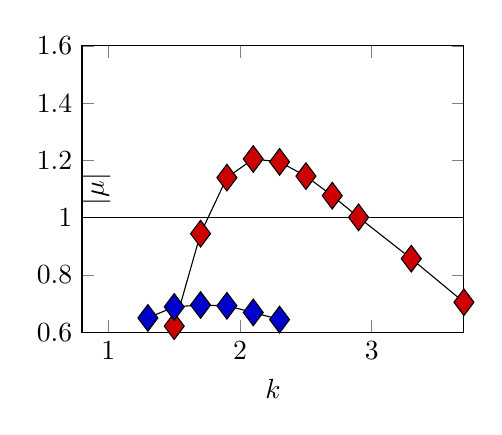
\begin{tikzpicture}



\begin{axis}[%
%width=4.3cm,
%height=3.5cm,
width=0.4\textwidth,
height=0.3\textwidth,
%width=0.2\textwidth,
%height=0.2\textwidth,
scale only axis,
%grid=both,
%axis lines=middle,
xmin=0.8,
xmax=3.7,
ymin=0.6,
ymax=1.6,
%xtick={2, 3, 4, 5, 6, 7, 8, 9, 10, 11},
%ytick={2, 2.5, 3, 3.5, 4, 4.5, 5, 5.5, 6, 6.5, 7},
%xlabel style={font=\color{white!15!black}},
xlabel={$k$},
ylabel={$|\mu|$},
ylabel style={at={(0.1,0.5)}},
%ymin=0,
%ymax=200,
axis background/.style={fill=white},
legend style={at={(0.99,0.85)}, anchor=east, legend cell align=left, align=left, fill=none, draw=none}
]


\addplot [color=black,solid,mark=diamond*,mark options={scale=2.4,black,fill=red!80!black}]
  table[row sep=crcr]{%
1.5 0.621431 \\
1.7 0.944234 \\
1.9 1.13979 \\
2.1 1.20487 \\
2.3 1.19477 \\
2.5 1.14503 \\
2.7 1.07689 \\
2.9 1.00122 \\
3.3 0.856827 \\
3.7 0.704753 \\
};
\addplot [color=black,solid,mark=diamond*,mark options={scale=2.4,black,fill=blue!80!black}]
  table[row sep=crcr]{%
1.3 0.650088 \\
1.5 0.688449 \\
1.7 0.695007 \\
1.9 0.692386 \\
2.1 0.669215 \\
2.3 0.644222 \\
};


%\addlegendentry{$Re=500$}

\addplot [color=black,solid,mark=,mark options={scale=2.4,black,fill=green!80!black}]
  table[row sep=crcr]{%
  0 1 \\
  5 1 \\
};





\end{axis}

\end{tikzpicture}%

%  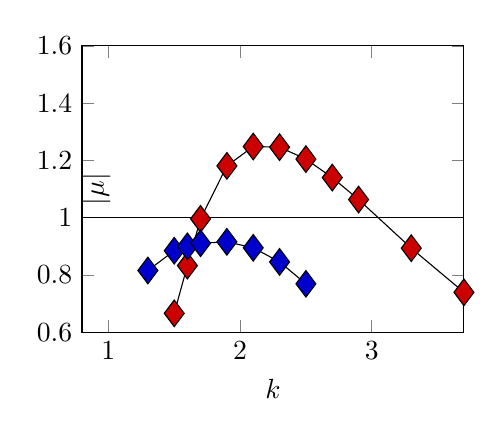
\begin{tikzpicture}



\begin{axis}[%
%width=4.3cm,
%height=3.5cm,
width=0.4\textwidth,
height=0.3\textwidth,
%width=0.2\textwidth,
%height=0.2\textwidth,
scale only axis,
%grid=both,
%axis lines=middle,
xmin=0.8,
xmax=3.7,
ymin=0.6,
ymax=1.6,
%xtick={2, 3, 4, 5, 6, 7, 8, 9, 10, 11},
%ytick={2, 2.5, 3, 3.5, 4, 4.5, 5, 5.5, 6, 6.5, 7},
%xlabel style={font=\color{white!15!black}},
xlabel={$k$},
ylabel={$|\mu|$},
ylabel style={at={(0.1,0.5)}},
%ymin=0,
%ymax=200,
axis background/.style={fill=white},
legend style={at={(0.99,0.85)}, anchor=east, legend cell align=left, align=left, fill=none, draw=none}
]


\addplot [color=black,solid,mark=diamond*,mark options={scale=2.4,black,fill=red!80!black}]
  table[row sep=crcr]{%
1.5 0.666004 \\
1.6 0.832646 \\
1.7 0.9958 \\
1.9 1.18082 \\
2.1 1.24832 \\
2.3 1.24618 \\
2.5 1.20433 \\
2.7 1.14004 \\
2.9 1.06321 \\
3.3 0.893504 \\
3.7 0.739385 \\
};
\addplot [color=black,solid,mark=diamond*,mark options={scale=2.4,black,fill=blue!80!black}]
  table[row sep=crcr]{%
1.3 0.815608 \\
1.5 0.884647 \\
1.6 0.899934 \\
1.7 0.910632 \\
1.9 0.915668 \\
2.1 0.89476 \\
2.3 0.845626 \\
2.5 0.769004 \\
%2.7 0.733247 \\
};


%\addlegendentry{$Re=500$}

\addplot [color=black,solid,mark=,mark options={scale=1.4,black,fill=green!80!black}]
  table[row sep=crcr]{%
  0 1 \\
  5 1 \\
};





\end{axis}

\end{tikzpicture}%
  
%  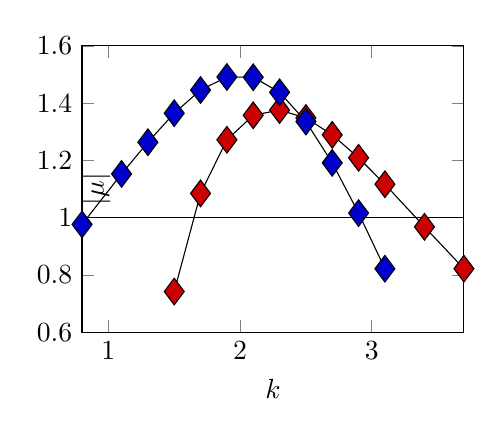
\begin{tikzpicture}



\begin{axis}[%
%width=4.3cm,
%height=3.5cm,
width=0.4\textwidth,
height=0.3\textwidth,
%width=0.2\textwidth,
%height=0.2\textwidth,
scale only axis,
%grid=both,
%axis lines=middle,
xmin=0.8,
xmax=3.7,
ymin=0.6,
ymax=1.6,
%xtick={2, 3, 4, 5, 6, 7, 8, 9, 10, 11},
%ytick={2, 2.5, 3, 3.5, 4, 4.5, 5, 5.5, 6, 6.5, 7},
%xlabel style={font=\color{white!15!black}},
xlabel={$k$},
ylabel={$|\mu|$},
ylabel style={at={(0.1,0.5)}},
%ymin=0,
%ymax=200,
axis background/.style={fill=white},
legend style={at={(0.99,0.85)}, anchor=east, legend cell align=left, align=left, fill=none, draw=none}
]


\addplot [color=black,solid,mark=diamond*,mark options={scale=2.4,black,fill=red!80!black}]
  table[row sep=crcr]{%
1.5 0.742066 \\
1.7 1.08482 \\
1.9 1.27188 \\
2.1 1.35744 \\
2.3 1.3757 \\
2.5 1.34816 \\
2.7 1.28908 \\
2.9 1.20902 \\
3.1 1.11666 \\
3.4 0.968 \\
3.7 0.821928 \\
};
\addplot [color=black,solid,mark=diamond*,mark options={scale=2.4,black,fill=blue!80!black}]
  table[row sep=crcr]{%
0.8 0.976452 \\
1.1 1.1528 \\
1.3 1.26332 \\
1.5 1.36481 \\
1.7 1.44557 \\
1.9 1.49116 \\
2.1 1.49023 \\
2.3 1.43771 \\
2.5 1.33553 \\
2.7 1.1913 \\
2.9 1.01607 \\
3.1 0.821755 \\
};


%\addlegendentry{$Re=500$}

\addplot [color=black,solid,mark=,mark options={scale=1.4,black,fill=green!80!black}]
  table[row sep=crcr]{%
  0 1 \\
  5 1 \\
};





\end{axis}

\end{tikzpicture}%

  \includegraphics[width=0.49\textwidth]{./fig/AR5s/multipliers_AR5.eps}
  \includegraphics[width=0.49\textwidth]{./fig/AR5s/multipliers_AR5p25.eps}  
  \includegraphics[width=0.49\textwidth]{./fig/AR5s/multipliers_AR5p5.eps}  
  \includegraphics[width=0.49\textwidth]{./fig/AR5s/multipliers_AR5p75.eps}      
  \vspace{0.1cm}
  \begin{tikzpicture}
  \draw (-10,2) -- (8,2);
  \end{tikzpicture}
  \vspace{0.1cm}
  \includegraphics[width=0.32\textwidth]{./fig/AR5s/Floqetmode_beta_2_Re550_AR5p5_A.png}
  \includegraphics[width=0.32\textwidth]{./fig/AR5s/Floqetmode_beta_2_Re550_AR5p5_QS.png} 
  \includegraphics[width=0.32\textwidth]{./fig/AR5s/Floqetmode_beta_4p75_Re550_AR5p5_Ap.png}
  \vspace{0.1cm}
  \begin{tikzpicture}
  \draw (-10,2) -- (8,2);
  \end{tikzpicture}
  \vspace{0.1cm}
  \includegraphics[width=0.49\textwidth]{./fig/AR5s/lambda2-AR55-Re450-3D.png}   
  \includegraphics[width=0.49\textwidth]{./fig/AR5s/lambda2-AR55-Re500-3D.png}     
  \caption{Top: Floquet multipliers for $\AR=5$ (top left), $\AR=5.25$ (top right), $\AR=5.5$ (bottom left) and $\AR=5.75$ (bottom right). The red symbols refer to mode $QS$. The blue symbols refer to mode $A$. The green symbols refer to mode $B$. Different symbols refer to different $Re$. Centre: Floquet modes associated with mode A (left), mode QS (centre) and mode $A'$ for $\AR=5.5$ and $Re=550$. Bottom: Results from the 3D DNS for $\AR=5.5$. Left: $Re=450$, right: $Re=500$. It is thus clear that mode A dominates at smaller $Re$, while once mode $QS$ becomes unstable it dominates. Mode $A'$ has the same symmetries of mode $A$ and is a synchronous mode. The difference is that its characteristic wavelength is much smaller, with $\beta_c \approx 4.5$. XX CHECK MODE GREEN FOR $AR=5.5$ and $Re=600$. POTREBBE ESSERE CHE SONO DUE MODI SEPARATI? XX}
  \label{fig:mult_AR5s}
\end{figure} 

\section{Bodies with $6 \le \AR \le 8$}

\begin{itemize}
  \item For these $\AR$, the secondary flow instability is due to mode $QS$ that leads to a three-dimensional state. Interestingly, for these $\AR$ mode $A$ is not detected. This is consistent with the fact that for this range of $\AR$, at the intermediate $Re$, the flow is driven by the LE vortex shedding, that modifies the flow dynamics in the near-wake region where the triggering mechanism of mode $A$ takes place. 
\end{itemize}

\begin{figure}
  \centering
  \includegraphics[width=0.49\textwidth]{./fig/AR7s/multipliers_AR6.eps}  
  \includegraphics[width=0.49\textwidth]{./fig/AR7s/multipliers_AR7.eps}
  \includegraphics[width=0.49\textwidth]{./fig/AR7s/multipliers_AR7_b.eps}
  \includegraphics[width=0.7\textwidth]{./fig/AR7s/Floqetmode_beta_2p2_Re500_AR7.png}
  \caption{Floquet stability analysis for $\AR=6$ and $\AR=7$. Top: Floquet multipliers associated with the unstable branch. for $\AR=6$ (left) and $\AR=7$ (right). Centre: dependence of the real and imaginary parts of $\mu$ on $\beta$ for $\AR=7$. Bottom: three-dimensional reconstruction of the unstable Floquet mode for $\AR=7$. For these $\AR$s the secondary instability of the flow is due mode $QS$.}
  \label{fig:mult_AR7s}
\end{figure}

\section{$\AR=9$}

\begin{figure}
  \centering
  \includegraphics[width=0.49\textwidth]{./fig/AR9s/Floquet_AR9_Re400_beta1p2_modeA.png}  
  \includegraphics[width=0.49\textwidth]{./fig/AR9s/Floquet_AR9_Re450_beta2_modeQS.png}
  \caption{Reconstruction of the Floquet modes for $\AR=9$. Left: mode $A$, $Re=400$, $\beta=1.2$. Right: mode $QS$, $Re=450$, $\beta=2$.}
  \label{fig:mult_AR9s}
\end{figure}

\section{Onset of mode A}

\begin{figure}
  \centering
  \includegraphics[width=0.49\textwidth]{./fig/LagTrac/part_AR1_Re200.eps}
  \includegraphics[width=0.49\textwidth]{./fig/LagTrac/part_AR4p5_Re410.eps}
  \includegraphics[width=0.49\textwidth]{./fig/LagTrac/part_AR5p75_Re550.eps}
  \includegraphics[width=0.49\textwidth]{./fig/LagTrac/part_AR7_Re500.eps}  
  \caption{XX AUMENTARE IL RANGE INVESTIGATO XX}
  \label{fig:part_res}
\end{figure}    

\begin{figure}
  \centering
  \includegraphics[width=0.49\textwidth]{./fig/LagTrac/orb_AR4p5_Re410.eps}   
  \includegraphics[width=0.49\textwidth]{./fig/LagTrac/orb_AR4p5_Re410.eps} 
  \includegraphics[width=0.49\textwidth]{./fig/LagTrac/orb_AR5p75_Re550.eps}
  \includegraphics[width=0.49\textwidth]{./fig/LagTrac/orb_AR7_Re500.eps}
  \caption{XX AUMENTARE IL RANGE INVESTIGATO XX}
  \label{fig:part_res}
\end{figure}    

\section*{Funding} 
This research received no specific grant from any funding agency, commercial or not-for-profit sectors.

\section*{Declaration of Interests} 
The authors report no conflict of interest.


\bibliographystyle{jfm}
\bibliography{Stability}


\end{document}



